%    Copyright 2017 Marc Demierre, HES-SO//Master
%
% Licensed under the Apache License, Version 2.0 (the "License");
% you may not use this file except in compliance with the License.
% You may obtain a copy of the License at
%
% http://www.apache.org/licenses/LICENSE-2.0
%
% Unless required by applicable law or agreed to in writing, software
% distributed under the License is distributed on an "AS IS" BASIS,
% WITHOUT WARRANTIES OR CONDITIONS OF ANY KIND, either express or implied.
% See the License for the specific language governing permissions and
% limitations under the License.

% =============================================================================
% | HES-SO//Master - Thesis project report template                           |
% |                                                                           |
% | Originally based on the EPFL template, with many adjustements             |
% =============================================================================

% Document settings
\documentclass[a4paper,11pt,fleqn,twoside,openright]{book}
\usepackage[utf8]{inputenc}
\usepackage[T1]{fontenc}
\usepackage[french,english]{babel}

% -----------------------------------------------------------------------------
% Preamble
% -----------------------------------------------------------------------------
% =============================================================================
% | Thesis metadata                                                           |
% =============================================================================

% Thesis info
\newcommand{\ThesisTitle}{GASP: Guide to Assess Security and Privacy levels on web services}
\newcommand{\ThesisSubject}{Master Thesis}
\newcommand{\Orientation}{Information and Communication Technologies (ICT)}
\newcommand{\Keywords}{IT Security, User Privacy, Confidentiality, Web Services, Data Science}

% Author
\newcommand{\AuthorFirstName}{Loïc}
\newcommand{\AuthorLastName}{\textsc{Guibert}}
\newcommand{\AuthorEmail}{loic.guibert@master.hes-so.ch}
\newcommand{\AuthorEmailBackup}{loicguib@ik.me}
\newcommand{\Author}{\AuthorFirstName\ \AuthorLastName}

% First Advisor
\newcommand{\SupervisorOneFirstName}{Pascal}
\newcommand{\SupervisorOneLastName}{\textsc{Bruegger}}
\newcommand{\SupervisorOneSchool}{HES-SO//Master}
\newcommand{\SupervisorOneResearchUnit}{HEIA-FR · iCoSys}
\newcommand{\SupervisorOne}{Dr. \SupervisorOneFirstName\ \SupervisorOneLastName}

% Second Advisor
\newcommand{\SupervisorTwoFirstName}{Adriana}
\newcommand{\SupervisorTwoLastName}{\textsc{Wilde}}
\newcommand{\SupervisorTwoSchool}{University of Winchester · WINTS}
\newcommand{\SupervisorTwoResearchUnit}{University of Southampton · CHT}
\newcommand{\SupervisorTwo}{Dr. \SupervisorTwoFirstName\ \SupervisorTwoLastName}

% Main expert
\newcommand{\ExpertFirstName}{Robert} 
\newcommand{\ExpertLastName}{\textsc{Van Kommer}} 
\newcommand{\Expert}{Dr. \ExpertFirstName\ \ExpertLastName}
\newcommand{\ExpertLab}{EPFL Innovation Park · Alliance}

% Internal expert
\newcommand{\ExpertInternalFirstName}{Jean} 
\newcommand{\ExpertInternalLastName}{\textsc{Hennebert}} 
\newcommand{\ExpertInternal}{Dr. \ExpertInternalFirstName\ \ExpertInternalLastName}

% Advisor
\newcommand{\Advisor}{Philippe \textsc{Joye}}

% Dean
\newcommand{\Dean}{Dr. Bernard \textsc{Masserey}}

% Place (for date and place)
\newcommand{\Date}{\today}
\newcommand{\Place}{Winchester (UK)}

\newcommand{\Researchquestion}{How to help organizations to evaluate their web services that also use \gls{ai} processes, by measuring the risk levels of both \gls{ict} security and user privacy concerns?}         % your project data
% ==================
% Template settings
% ==================

% General tools
% -------------
\usepackage{etoolbox}

% Page style
% ----------
\usepackage[margin=3cm, left=3.5cm, right=3.5cm, twoside=true]{geometry}
\usepackage{fancyhdr}
\setlength{\headheight}{14pt}
\renewcommand{\sectionmark}[1]{\markright{\thesection\ #1}}
\pagestyle{fancy}

% Standard pages (inside chapters)
\fancyhf{}
\renewcommand{\headrulewidth}{0.4pt}
\renewcommand{\footrulewidth}{0pt}
\fancyhead[OR]{\bfseries \nouppercase{\rightmark}}
\fancyhead[EL]{\bfseries \nouppercase{\leftmark}}
\fancyfoot[EL,OR]{\thepage}

% First page of chapters
\fancypagestyle{plain}{
	\fancyhf{}
	\renewcommand{\headrulewidth}{0pt}
	\renewcommand{\footrulewidth}{0pt}
	\fancyfoot[EL,OR]{\thepage}
}

% Imports for external PDFs
\fancypagestyle{addpagenumbersforpdfimports}{
	\fancyhead{}
	\renewcommand{\headrulewidth}{0pt}
	\fancyfoot{}
	\fancyfoot[RO,LE]{\thepage}
}

% Use empty style for page when clearing double pages
\def\cleartoodd{%
	\clearpage%
	\ifodd\value{page}\else\mbox{}\thispagestyle{empty}\newpage\fi%
}

\def\clearchap{%
	\ifodd\value{page}\else\mbox{}\thispagestyle{empty}\fi%
}

% \cleardoublepage replaced by \cleartoodd
\let\origdoublepage\cleardoublepage
\renewcommand{\cleardoublepage}{%
	\cleartoodd%
}

% Fonts
% -----

% Helvetica (Arial used in the MSE Word template)
\usepackage{helvet}

% Math
% ----
\usepackage{amsmath}  % better math

% Floats and figures
% ------------------
\usepackage{newfloat}          % floats
\usepackage[twoside]{caption}  % captions
\usepackage{subcaption}        % subcaptions
\usepackage[section]{placeins} % allows to put float barriers

% Float captions in italics, with label in margin
\DeclareCaptionLabelFormat{title}{#1 #2}
\DeclareCaptionLabelFormat{hangout}{\llap{#1 #2\hspace{5mm}}}
\captionsetup{
	format=hang,
	labelformat=hangout,
	singlelinecheck=false,
	font={it}
}

% Caption with source for figure
% TODO: improve this to use square brackets like the normal "caption"
\newcommand*{\captionsource}[3]{%
\caption[{#1}]{%
	#2%
	
	\textbf{Source:} #3%
}%
}

% Tables
% ------
\usepackage{booktabs} % much better tables
\usepackage{multirow} % allows to fuse rows
\usepackage{array}    % manipulate array
\usepackage{tabularx} % better tables

% Define new tabularx column types:
%  - R: streteched right aligned
%  - C: stretched centered
%  - N: left aligned, specified space
\newcolumntype{R}{>{\raggedleft\arraybackslash}X}%
\newcolumntype{C}{>{\centering\arraybackslash}X}%
\newcolumntype{N}[1]{>{\raggedleft\arraybackslash}p{#1}}

% Set row height multiplicator to provide more breathing space
\renewcommand{\arraystretch}{1.3} 

% Bibliography
% -------------------

% Use biber, with numeric style and no sorting (citation order)
\usepackage[
backend=biber,
style=numeric,
sorting=none,
bibencoding=auto
]{biblatex}
\addbibresource{03-tail/bibliography.bib}


% Tables of contents, figures, tables and listings
% ------------------------------------------------
\usepackage{tocloft}
\newlistof{listing}{lol}{List of Listings}
\setcounter{tocdepth}{1} % Depth to 'section'
\setlength{\cftfigindent}{0pt}  % remove indentation from figures in lof
\setlength{\cftfignumwidth}{1cm}
\setlength{\cfttabindent}{0pt}  % remove indentation from tables in lot
\setlength{\cfttabnumwidth}{1cm}
\setlength{\cftlistingindent}{0pt}
\setlength{\cftlistingnumwidth}{1cm}

% Mini tables of contents
% -----------------------
\usepackage{minitoc}

% no "Contents" title
\mtcsettitle{minitoc}{Contents} 

% Layout
\setlength{\mtcindent}{-0.5em}
\mtcsetoffset{minitoc}{-1em}

% Spacing above and below table
\mtcsetfeature{minitoc}{before}{\vspace{0.5cm}}
\mtcsetfeature{minitoc}{after}{\vspace{-0.25cm}}
\renewcommand{\mtifont}{\sffamily\bfseries\large}
\renewcommand{\mtcSfont}{\sffamily\bfseries\small}
\renewcommand{\mtcSSfont}{\sffamily\small}
\renewcommand{\mtcSSSfont}{\sffamily\small}

% Colors & graphics
% -----------------
\usepackage[table]{xcolor}    % colors
\usepackage[pdftex]{graphicx} % graphics importing
\graphicspath{{02-main/figures/}}
\definecolor{gray80}{gray}{0.80}


% Code and syntax highlighting
% ----------------------------
\usepackage[newfloat]{minted}   % code highlighting

% Typography
% ----------
\usepackage{csquotes}                    % paragraph indentation and spacing
\usepackage[defaultlines=3,all]{nowidow} % avoid widows and orphans
\usepackage{microtype}                   % typographic improvements
\usepackage{parskip}                     % No indent and auto-space between paragraphs
\usepackage[super]{nth}

\usepackage{paralist}
\usepackage{enumitem}
%\setlist{after=\vspace{\baselineskip}} % Modified

% Section and chapters headings
% -----------------------------
\usepackage[explicit]{titlesec} % titles formatting
%\usepackage{titletoc} % titles formatting in ToC etc
%\usepackage{sectsty}  % sectioning commands

% -- Chapters --
% Remove "Chapter N" and use a sans-serif font

% Set layout lengths
\setlength{\headheight}{8mm}
\setlength{\footskip}{1.5cm}
\addtolength{\textheight}{-.5cm}

\titlespacing{\chapter}{-5mm}{-10mm}{3mm}
\titlespacing{\section}{-5mm}{3mm}{-2mm}
\titlespacing{\subsection}{-5mm}{2mm}{-2mm}
\titlespacing{\subsubsection}{-5mm}{2mm}{-1mm}


%\titleformat{\chapter}[block]
%{\Huge}
%{\thechapter\hspace{12pt}\textcolor{gray80}{|}\hspace{12pt}}
%{0pt}
%{\Huge\bfseries}

\titleformat{\chapter}{\Huge\bfseries}{\llap{\thechapter\hspace{12pt}\textcolor{gray80}{|}}}{0mm}{%
	\hfill\begin{minipage}[t]{\dimexpr\textwidth}\raggedright#1\end{minipage}%
}
\titleformat{\section}{\Large\bfseries}{\llap{\thesection}}{0mm}{%
	\hfill\begin{minipage}[t]{\dimexpr\textwidth}\raggedright#1\end{minipage}%
}
\titleformat{\subsection}{\large \bfseries}{\llap{\thesubsection}}{0mm}{%
	\hfill\begin{minipage}[t]{\dimexpr\textwidth}\raggedright#1\end{minipage}%
}
\titleformat{\subsubsection}{\bfseries}{\llap{\thesubsubsection}}{0mm}{%
	\hfill\begin{minipage}[t]{\dimexpr\textwidth}\raggedright#1\end{minipage}%
}

% Misc
% ------
\usepackage{lipsum}    % filler text
\usepackage{blindtext} % random text
\usepackage{lscape}    % easy landscape pages
\usepackage{pdflscape} % landscape pages for PDFs

% Allow email typesetting
\newcommand{\email}[1]{
	\href{mailto:#1}{\textit{#1}}
}

% References
% -----------
\usepackage{url}

 %pdf metadata
\usepackage{hyperref}
\hypersetup{pdftitle={\ThesisTitle},pdfauthor={\Author},pdfsubject={\ThesisSubject},pdfkeywords={\Keywords}}

% % Hyperlinks
% \hypersetup{
% 	colorlinks=true,
% 	linkcolor=black,
% 	citecolor=black,
% 	filecolor=black,
% 	urlcolor=black,
% }

\providecommand*{\listingautorefname}{Listing}


% Glossary
% --------
\usepackage[xindy,toc]{glossaries}
% ==============================================================================
% = Personal glossary of Loïc Guibert, free to use. Used across several projects
% ==============================================================================


% Terms
% -----
% format:  \newglossaryentry{<label>}{<settings>}
% example: \newglossaryentry{computer}
%{
%	name=computer,
%	description={is a programmable machine that receives input,
%		stores and manipulates data, and provides
%		output in a useful format}
%}

\newglossaryentry{backend}{
  name={backend},
  description={The part of a software program that includes its logic layer, which is to generate one or more results from operations. Not visible to users}
}
\newglossaryentry{blockchain}{
	name={blockchain},
	description={A dynamic list of data grouped in \textit{blocks} linked by cryptography mechanisms. Each block brings additional data to the chain and validates the previous block's integrity}
}

\newglossaryentry{cookie}{
  name={cookie},
  description={A cookie is a pair, composed by a key and a value, that is stored on a client's Web browser. It is linked to one or many websites and are used as way to provide stateful information to the website between visits, such as a session identifier}
}
\newglossaryentry{ciphertext}{
  name={ciphertext},
  description={A term used to describe any \gls{plaintext} that has been encryptedby an algorithm. It is not readable without a prior decryption process}
}
\newglossaryentry{cloud}{
  name={cloud},
  description={An architectural model where computing resources are made available to the user without direct active management. Usually describes data centres that are accessible to many users over the Internet}
}
\newglossaryentry{cluster}{
  name={cluster},
  description={A set of computers that work together. Each node have the same task and the whole set can be viewed as a single system}
}

\newglossaryentry{framework}{
	name={framework},
	description={A framework is a set of software components used to bring new possibilities for the development of an IT tool, especially by providing elements related to its infrastructure. Outside of the \gls{it} field, it describes a set of rules, practices or must-haves in order to achieve a goal}
}
\newglossaryentry{frontend}{
  name={frontend},
  description={The part of a software program that includes its graphical presentation layer, which is presented to users}
}

\newglossaryentry{json}{
  name={JSON},
  description={JavaScript Object Notation: a file format widely used for sending information between different information systems. Its structure is very simple and is easily readable by humans}
}

\newglossaryentry{homomorphism}{
  name={homomorphism},
  description={An algebra term which is a mapping between two algebraic structures of the same type}
}

\newglossaryentry{kernel}{
  name={kernel},
  description={One of the fundamental parts of most \glspl{os}. It manages the computer's resources and allows hardware and software components to communicate with each other. One of the most used kernel is \gls{linux}}
}

\newglossaryentry{linux}{
  name={Linux},
  description={Also known as \gls{gnu}/Linux. A family of open source \gls{unix}-like \glspl{os} based on the Linux \gls{kernel}. Numerous Linux distributions have integrated this Linux in their structure and can be used for a wide variety of tasks}
}
\newglossaryentry{lstm}{
  name={Long Short-Term Model},
  description={A \gls{rnn} using units that partially solve the vanishing gradient problem. Allows gradients to flow unchanged if needed}
}

\newglossaryentry{neural network}{
  name={Neural Network},
  description={Network or circuit of artificial neurons that imitates structure of biological brains. It is used for solving artificial intelligence problems}
}
\newglossaryentry{nosql}
{
	name=NoSQL,
	description={Database not using the relational model and the \acrshort{sql} language}
}

\newglossaryentry{opensource}
{
	name={open-source},
	description={The fact to freely share the source code used to build a program to the public, generally associated with a licence. It is also a movement}
}

\newglossaryentry{package_manager}{
  name={package manager},
  description={A package manager is one or several softwares which permit to automate management actions on computer programs. It can install, upgrade, configure and remove them with a understanding of dependencies and compatibility between each others}
}
\newglossaryentry{plaintext}{
  name={plaintext},
  description={A term used to describe any data that is not encrypted and readable by an information system or a human}
}

\newglossaryentry{quic}{
  name={QUIC},
  description={Protocol that aims to replace \gls{tcp} by using some mecanisms from \gls{udp}. Some new features enable better performances, a latency decrease and a non-blocking re-transmission of lost packets}
}

\newglossaryentry{relu}{
  name={ReLU},
  description={An activation function defined as zero for negative inputs and the input value for positive ones. Acts as a ramp function}
}
\newglossaryentry{rest}{
  name={REST},
  description={A set of guidelines for the architecture of an \acrshort{api}, to ensure interoperability between information systems on the Internet}
}
\newglossaryentry{rnn}{
  name={Recurrent Neural Network},
  description={A neural network with connections between nodes that form a directed graph along a temporal sequence}
}

\newglossaryentry{scrum}{
	name={Scrum},
	description={Project management approach that aims to divide the work into sprints, with tasks defined by the team}
}
\newglossaryentry{sgd}{
  name={Stochastic Gradient Descent},
  description={An iterative method for optimizing an objective function with suitable smoothness properties. It can be interpreted as an approximation of the general gradient descent optimization}
}
\newglossaryentry{sigmoid}{
  name={sigmoid},
  description={A function having a S-shaped curve. Often used for probability distribution on a deep-network output layer}
}

\newglossaryentry{tcb}{
    name={TCB},
    description={Includes all hardware, firmware, and software part of a system that are necessary and critical for the system security policy}
}
\newglossaryentry{token}{
    name={token},
    description={A token is a string of characters issued to users by an entity, allowing it to identify the authors of queries within their information system. In general, a token is unique and can be revoked. It is a kind of label, rarely in human-readable form}
}
\newglossaryentry{toolkit}{
    name={toolkit},
    description={Refers to an utility program, several software capabilites or a complete integrated set of software utilities which can be used to develop and maintain applications}
}

\newglossaryentry{unix}{
    name={UNIX},
    description={A family of multi-tasking, multi-user \glspl{os} derived from the original Unix created by \citeproper{AT&T} in the 1970s. It is based on an interpreter or supervisor named the shell and small utilities, each performing a specific action}
}

\newglossaryentry{websocket}{
  name={WebSocket},
  description={A communication protocol that provides full-duplex (bidirectional) communication channels over a single TCP connection. It therefore allows information to be sent to and from servers}
}
\newglossaryentry{white-paper}{
  name={white paper},
  description={A report or guide that present concise information on a complex subject while presenting the author's principles. It is usually intended to facilitate or guide the reader's decision making on the subject, and is used at both institutional and commercial levels}
}



% Acronyms
% --------
% format:  \newacronym{<label>}{<abbrv>}{<full>}
% example: \newacronym{lvm}{LVM}{Logical Volume Manager}
% plural:  \newacronym[longplural={Frames per Second}]{fpsLabel}{FPS}{Frame per Second}

\newacronym{api}{API}{Application Programming Interface}
\newacronym{ai}{AI}{Artificial Intelligence}

\newacronym{ccpa}{CCPA}{California's Consumer Privacy Act}
\newacronym{cep}{CEP}{Complex Event Processing}
\newacronym{ca}{CA}{Certificate Authority}
\newacronym{ci}{CI}{Continuous Integration}
\newacronym{cms}{CMS}{Content Management System}
\newacronym{cqrs}{CQRS}{Command Query Responsibility Segregation}
\newacronym{crud}{CRUD}{Create-Read-Update-Delete}
\newacronym{css}{CSS}{Cascading Style Sheets}

\newacronym{dag}{DAG}{Directed Acyclic Graph}
\newacronym{darpa}{DARPA}{Defense Advanced Research Projects Agency}
\newacronym{dl}{DL}{Deep Learning}
\newacronym{dom}{DOM}{Document Object Model}
\newacronym{dprive}{DPRIVE}{Data Protection in Virtual Environments}
\newacronym{dsl}{DSL}{Domain Specific Language}

\newacronym{eca}{ECA}{Event Condition Action}
\newacronym{elk}{ELK}{Elasticseach Logstash and Kibana}
\newacronym{efk}{EFK}{Elasticseach Fluentd and Kibana}
\newacronym{epa}{EPA}{Event Processing Agent}
\newacronym{epn}{EPN}{Event Processing Network}

\newacronym{fhe}{FHE}{Fully Homomorphic Encryption}
\newacronym{fc}{FC}{Fully Connected}

\newacronym{gdpr}{GDPR}{General Data Protection Regulation }
\newacronym{gelf}{GELF}{Graylog Extended Log Format}
\newacronym{ge}{GE}{Generic Enabler}
\newacronym{gnu}{GNU}{GNU's Not \gls{unix}} %TODO mix glossary and acronym

\newacronym{heia}{HEIA-fr}{School of Engineering and Architecture of Fribourg}
\newacronym{http}{HTTP}{Hypertext Transfer Protocol}
\newacronym{https}{HTTPS}{\glsentryshort{http} Secure}
\newacronym{httpa}{HTTPA}{\glsentryshort{https} Attestable}

\newacronym{ide}{IDE}{Integrated Development Environment}
\newacronym{ietf}{IETF}{Internet Engineering Task Force}
\newacronym{iot}{IoT}{Internet of Things}
\newacronym{ip}{IP}{Internet Protocol}
\newacronym{it}{IT}{Informational Technologies}

\newacronym{jar}{JAR}{Java ARchive}
\newacronym{jmx}{JMX}{Java Management Extensions}
% \newacronym{json}{JSON}{JavaScript Object Notation} TODO: combine with glossary entry
\newacronym{jvm}{JVM}{Java Virtual Machine}

\newacronym{lfhe}{LFHE}{Leveled fully homomorphic encryption}

\newacronym{ml}{ML}{Machine Learning}
\newacronym[longplural={MultiLayer Perceptrons}]
{mlp}{MLP}{MultiLayer Perceptron}
\newacronym{mpc}{MPC}{Multi-Party Computation}
\newacronym{mvc}{MVC}{Model - View - Controller}

\newacronym{npm}{NPM}{Node Package Manager (unofficial name)}
\newacronym[longplural={Neural Networks}]
{nn}{NN}{Neural Network}

\newacronym{os}{OS}{Operating System}
\newacronym{osi}{OSI}{Open Systems Interconnection}

\newacronym{phe}{PHE}{Partially Homomorphic Encryption}
\newacronym{pal}{PAL}{Platform Adaptation Layer}
\newacronym{psp}{PSP}{Platform Security Processor}
\newacronym[longplural={Proofs of Concept}]
{poc}{PoC}{Proof of Concept}

% \newacronym{rest}{REST}{Representational state transfer} TODO: combine with glossary entry
\newacronym{rest_markup}{reST}{reStructuredText}
\newacronym{rfc}{RFC}{Request for Comments}
\newacronym{rpc}{RPC}{Remote Procedure Call}

\newacronym{sdk}{SDK}{Software Development kit}
\newacronym{sgx}{SGX}{Software Guard Extensions}
\newacronym{sql}{SQL}{Structured Query Language}
\newacronym{ssh}{SSH}{Secure Shell}
\newacronym{ssl}{SSL}{Secure Sockets Layer}
\newacronym{swhe}{SWHE}{Somewhat Homomorphic Encryption}

\newacronym{tls}{TLS}{Transport Layer Security}
%\newacronym{tcb}{TCB}{Trusted computing base} TODO: combine with gls
\newacronym{tcp}{TCP}{Transmission Control Protocol}
\newacronym{tdx}{TDX}{Trust Domain Extensions}
\newacronym[
longplural={Trusted Execution Environments}]
{tee}{TEE}{Trusted Execution Environment}
\newacronym{txt-intel}{TXT}{Trusted Execution Technology}
\newacronym{tpm}{TPM}{Trusted Platform Module}

\newacronym{uuid}{UUID}{Universally Unique Identifier}
\newacronym{udp}{UDP}{User Datagram Protocol}
\newacronym{ui}{UI}{User Interface}
\newacronym{uri}{URI}{Universal Resource Identifier}

\newacronym{vm}{VM}{Virtual Machine}

\makeglossaries

    % template settings
% LTeX: enabled=false

% ===========================================
% = Codestyles for minted syntax highlighting
% ===========================================


% How to use (replace 'java' with language name):
% - code blocks:
%     \begin{javacode}
%     CODE
%     \end{javacode}
% - files:
%     full: \javafile{PATH}
%     extract: \javafile[startline=x, endline=y]{PATH}


% Javascript
\newminted{javascript}{frame=single, framesep=6pt, breaklines=true, fontsize=\scriptsize, linenos, autogobble}
\newmintedfile{javascript}{frame=single, framesep=6pt, breaklines=true, 
fontsize=\scriptsize, linenos, autogobble}

% Python
\newminted{python}{frame=single, framesep=6pt, breaklines=true, fontsize=\scriptsize, linenos, autogobble}
\newmintedfile{python}{frame=single, framesep=6pt, breaklines=true, fontsize=\scriptsize, linenos, autogobble}

% Json
\newminted{json}{frame=single, framesep=6pt, breaklines=true, fontsize=\scriptsize, linenos}
\newmintedfile{json}{frame=single, framesep=6pt, breaklines=true, 
	fontsize=\scriptsize, linenos}

% Plain text
\newminted{text}{frame=single, framesep=6pt, breaklines=true, breakanywhere, fontsize=\scriptsize, linenos}
\newmintedfile{text}{frame=single, framesep=6pt, breaklines=true, breakanywhere, fontsize=\scriptsize, linenos}

% LTeX: enabled=true       % code styles for minted
% ========================
% Lighter settings
% ========================

% Marc's font stack
\usepackage{cmbright}       % Sans serif
\usepackage{sourcecodepro}  % Monospace
\renewcommand{\familydefault}{\sfdefault}

\titlespacing{\section}{-5mm}{5mm}{2mm}
\titlespacing{\subsection}{-5mm}{2mm}{1mm}
\titlespacing{\subsubsection}{-5mm}{2mm}{1mm}

% Colors and links - https://en.wikibooks.org/wiki/LaTeX/Hyperlinks
\usepackage{xcolor}% http://ctan.org/pkg/xcolor
\usepackage{hyperref}% http://ctan.org/pkg/hyperref
\hypersetup{
  colorlinks=true,
  linkcolor=blue!50!blue,
  urlcolor=blue!70!blue,
  citecolor=blue!70!blue
%	colorlinks=false,% hyperlinks will be black
%	linkbordercolor=blue,% hyperlink borders will be red
%	pdfborderstyle={/S/U/W 1}% border style will be underline of width 1pt
}

% First acroynm long
\renewcommand*{\CustomAcronymFields}{%
  name={\the\glsshorttok},% name is abbreviated form
  description={\the\glslongtok},% description is long form
  first={\noexpand\emph{\the\glslongtok}\space(\the\glsshorttok)},%
  firstplural={\noexpand\emph{\the\glslongtok\noexpand\acrpluralsuffix}\space(\the\glsshorttok)},%
  text={\the\glsshorttok},%
  plural={\the\glsshorttok\noexpand\acrpluralsuffix}%
}

% To print date in custom command citeproperref
\usepackage[en-GB]{datetime2}

\glsenablehyper

% To continue numbering of footnotes in chapters
% https://tex.stackexchange.com/questions/10448/continuous-footnote-numbering
\counterwithout{footnote}{chapter}

% To suppress errors on custom font sizes
% https://tex.stackexchange.com/questions/58087/how-to-remove-the-warnings-font-shape-ot1-cmss-m-n-in-size-4-not-available
\usepackage{lmodern}

% To import PDF files as content
\usepackage{pdfpages}

% Long tables
\usepackage{ltablex}
\usepackage{booktabs}

% inline citations
\usepackage[
    left = `,%
    right = ',%
    leftsub = ``,%
    rightsub = ''%
]{dirtytalk}

% lighter color
% https://stackoverflow.com/questions/2516976/latex-making-a-lighter-version-of-text-like-anti-bold
\usepackage{color}
\definecolor{light}{rgb}{0.4, 0.4, 0.4}
\def\light#1{{\color{light}#1}}

% change name of the hyperref
% https://tex.stackexchange.com/questions/370991/change-chapter-to-chapter-how-to-do-this-using-autoref/370997#370997
\addto\extrasenglish{%
  \def\chapterautorefname{Chapter}%
  \def\sectionautorefname{Section}%
  \def\subsectionautorefname{Subsection}%
  \def\subsubsectionautorefname{Subsubsection}%
  \def\paragraphautorefname{Paragraph}%
  \def\subparagraphautorefname{Subparagraph}%
}

% Symbols
% https://www.latex4technics.com/?note=22y9
\usepackage{pifont}% http://ctan.org/pkg/pifont
\newcommand{\cmark}{\ding{51}}%
\newcommand{\xmark}{\ding{55}}%

% table spacing 
% https://tex.stackexchange.com/questions/381718/how-to-remove-the-space-after-midrule-in-a-table
\aboverulesep = 0mm \belowrulesep = 0mm  % your custom packages etc
\newcommand{\itembullet}{\begin{itemize}[label={•}]}

\newcommand{\newimage}[4]{
\begin{figure}[!h]
    \begin{center}
        \includegraphics[width=#1\textwidth]{#2}
        \caption{#3}
        \label{fig:#4}
    \end{center}
\end{figure}
}

%TODO Improve with inclusion of the basic form
\newcommand{\newsourcedimage}[8]{
\begin{figure}[!h]
    \begin{center}
        \includegraphics[width=#1\textwidth]{#2}
        %\caption{#3\\\hspace{\textwidth}Source: \url{#4} (accessed \DTMdisplaydate{#5}{#6}{#7}\\)}
        \captionsourcedated{#3}{\url{#4}}{#5}{#6}{#7}
        \label{fig:#8}
    \end{center}
\end{figure}
}

\newcommand{\fullrefname}[1]{\ref{#1} (\nameref*{#1})}
\newcommand{\fullrefnametype}[1]{\autoref{#1} (\nameref*{#1})}
% TODO fix this \newcommand{\Fullrefnametype}[1]{\expandafter\MakeUppercase A}
\newcommand{\Fullrefnametype}[1]{\fullrefnametype{#1}}

\newcommand{\citeproper}[1]{\textit{#1}}
\newcommand{\citeproperref}[5]{\citeproper{#1}\footnote{\textit{#1} source: \url{#2} \accessed{#3}{#4}{#5}}}

% --- Code and minted

% \newenvironment{codeBloc}[3]{
%     \begin{listing}[!ht]
%         \begin{minted}{#1}
%             ...
%         \end{minted}    
%         \caption{#2}
%         \label{listing:#3}
%     \end{listing}
% }

% \newenvironment{codeBloc}[1]
%     {[2]
%     {\end{minted}\caption{#1}\label{listing:#2}\end{listing}}

\newcommand{\codefile}[4]{
    \begin{listing}[!ht]
        \inputminted{#1}{#4}
        \caption{#2}
        \label{listing:#3}
    \end{listing}
}


\newcommand*{\captionsourcedated}[5]{%
\caption[{#1}]{%
	#1%
	
    \textit{Source:} #2%
    \
    \accessed{#3}{#4}{#5}%
	}%
}


\newcommand{\accessed}[3]{%
(accessed \DTMdisplaydate{#1}{#2}{#3}\\)
}         % custom commands

\begin{document}
% -----------------------------------------------------------------------------
% Front matter
% -----------------------------------------------------------------------------
\frontmatter

\dominitoc

% ==========================================================================
% = HES-SO Master thesis title page (modeled after Word template, 2016-2017)
% ==========================================================================

\begin{titlepage}
\newgeometry{margin=2.5cm}
{\fontfamily{phv}\fontseries{mc}\selectfont
	\begin{flushright}
		\begin{minipage}{0.33\textwidth}
			\begin{flushleft}
				
\includegraphics[width=1\textwidth]{img/mse_logo}
			\end{flushleft}
		\end{minipage}%
		\begin{minipage}{0.34\textwidth}
			\begin{center}
				
\includegraphics[width=1\textwidth]{img/hesso_logo.png}
			\end{center}
		\end{minipage}%
		\begin{minipage}{0.33\textwidth}
			\begin{flushright}
				
\includegraphics[width=1\textwidth]{img/winchester_logo}
			\end{flushright}
		\end{minipage}
		\begin{flushleft}
			\footnotesize
			Master of Science HES-SO in Engineering \\
			Av. de Provence 6 \\
			CH-1007 Lausanne
		\end{flushleft}
		~\\[1cm]
		
		{
		\Huge Master of Science HES-SO in Engineering\\[0.5cm]
		}
		
		{
		\LARGE \Orientation\\[1.5cm]
		}
		% Title
		{
			\Huge
			\textbf{\ThesisTitle} \\[0.5cm]
		}
		{
			\LARGE
			Supported by the Department of Digital Technologies \\
			at the University of Winchester, UK \\[1.5cm]
		}
		{
			\large
			\light{Author}\\[-0.3cm]
			\Huge \Author \\[1.5cm]
		}
		{
			\large
			\light{Supervisors} \\
			\SupervisorOne \\
			\textit{\SupervisorOneSchool, \\ \SupervisorOneResearchUnit} \\
			\light{and} \\
			\SupervisorTwo \\
			\textit{\SupervisorTwoSchool, \\ \SupervisorTwoResearchUnit} \\[0.5cm]
		}
		{
			\large
			\light{External expert} \\
			\Expert \\
			\textit{\ExpertLab}
		}
		
		\vfill
		
		% Bottom of the page
		{\large \Place, HES-SO//Master, \Date}
		
	\end{flushright}
}
\restoregeometry
\end{titlepage}

% Page for student info and signatures
\cleardoublepage
\chapter*{Information about this report}

\vspace{\fill}

\textbf{Contact information}

\begin{tabularx}{\textwidth}{N{2.5cm}X}
	Author:	 & \Author \\
	& MSE Student \\
	& HES-SO//Master \\
	& Switzerland \\
	Email: & \email{\AuthorEmail}
\end{tabularx}

\vspace{\fill}

\textbf{Declaration of honour}

{\renewcommand{\arraystretch}{2}
\begin{tabularx}{\textwidth}{N{2.5cm}X}
	& I, undersigned, \Author, hereby declare that the work submitted is 
	the result of a personal work. I certify that I have not resorted to 
	plagiarism or other forms of fraud. All sources of information used, and the 
	author quotes were clearly mentioned. \\
	%Place, date: & \underline{\hspace{7cm}} \\ % TODO
	Place, date: & \Place, \Date \\ 
	Signature: & \underline{\hspace{7cm}}
\end{tabularx}
}

\vspace{\fill}

% \textbf{Experts}

% \begin{tabularx}{\textwidth}{N{2.5cm}X}
% 	Advisor:	 & \Advisor \\
% 	Dean: & \Dean
% \end{tabularx}

% \vspace{\fill}

\textbf{Validation}

Accepted by the HES-SO//Master (Switzerland, Lausanne) on a proposal from:

\vspace{0.5cm}

\AdvisorOne and \AdvisorTwo, Thesis Project advisors

\vspace{1cm}

Place, date: \underline{\hspace{8cm}}

\vspace{3cm}

{ \renewcommand{\arraystretch}{1.5}
\begin{tabularx}{\textwidth}{X X X}
	\AdvisorOne, \AdvisorTwo  & \Dean\\ 
	Advisors &   & Dean, HES-SO//Master\\
\end{tabularx}
}

% Acknowledgments (your dedication etc)
\cleardoublepage
\chapter*{Acknowledgments}
\addcontentsline{toc}{chapter}{Acknowledgments}

This thesis would not have been possible without the support of many people. First, I am extremely grateful to my supervisor \SupervisorOne, who always supported me both in my whole education curriculum and through this thesis.

I also want to thank my other supervisor \SupervisorTwo, who accepted me as a visiting researcher and welcomed me at the University of Winchester. I am also very grateful for her supervision throughout my whole thesis despite her many obligations.

Thanks to the HES-SO//Master for allowing students to design and propose their own thesis subjects, and to ensure that the appropriate resources are provided.

And finally, I want to thank my parents, my sister, and my numerous friends who always supported me, not only during this thesis but also during my whole life. 

% Abstract
\cleardoublepage
\chapter*{Abstract}
\addcontentsline{toc}{chapter}{Abstract}

The vast majority of Internet users around the world accesses web services, for both personal and professional goals, often involving sensitive information. Therefore, web services must be secure to prevent attacks resulting from vulnerabilities being exploited. Against this background, recent advances in data science and Artificial Intelligence (AI) have led to an increased adoption of personalized, adaptive and customizable models in many areas, including in web services. However, these models need vast amounts of user data to achieve a satisfactory performance,  raising important privacy concerns. Therefore, it is critical for organizations to ensure that the web services they provide are both developed securely and designed respectfully of the privacy of their end users.  

This thesis addresses such need by providing an accessible, simple, and complete guide to evaluate web services for organizations. To meet this goal, we conducted a state-of-the-art review on multiple \acrlong*{ict} fields related to both the web environment and big data, focusing on security and privacy concerns. In addition, an evaluation of reputable existing guides (by NIST, NCSC, ENISA and CISA) was conducted to identify the gaps regarding web services, which informed the scope  for the development of this new guide. Several guidelines were then developed to allow organizations to assess whether their web services are compliant with recommendations, mitigations or other useful information, incorporating the  knowledge collected. Finally, an online web application has been developed specifically for a dynamic assessment of web services by organizations, against the entire knowledge collection we made in an easy, complete, efficient and accessible manner. The application, hosted at \href{https://ohmygasp.com}{ohmygasp.com}, allows organizations to receive heuristic scores  on the security and privacy levels of their assessed web services, on multiple categories. Those scores and the requirement levels specified for the knowledge collection are provided in order to give the organization a prioritized list on the most sensitive concerns, in order to quickly activate levers to strengthen their web services. The accuracy of our proposal and guide has been reviewed by assessing an existing web service, which suggests that our approach is not only valid  but also useful.

In its present form, the use of this guide already can benefit any organization developing web services. However, in addition, its generic design allows it to be extended for evaluations of systems from other contexts using customized guide contents, and therefore having the potential to become a centralized or decentralized hub that could store, compare and help design  guide contents for various subjects, scopes or technologies. This growth would allow us to improve the security and privacy levels of many more systems.

\vskip0.5cm
\textbf{Keywords:} 
\Keywords

% Table of contents
\cleardoublepage
\phantomsection
\addcontentsline{toc}{chapter}{Contents}
\tableofcontents

% List of figures
\cleardoublepage
\phantomsection
\addcontentsline{toc}{chapter}{List of Figures}
\listoffigures

% List of tables
\cleardoublepage
\phantomsection
\addcontentsline{toc}{chapter}{List of Tables}
\listoftables

% List of listings
\cleardoublepage
\phantomsection
\addcontentsline{toc}{chapter}{List of Listings}
\listoflistings

% Restore paragraphs
\setlength{\parskip}{1em}

% Bold fonts for sections in minitoc
\renewcommand{\cftsecfont}{\sffamily\bfseries}
\renewcommand{\cftsecleader}{\sffamily\bfseries\cftdotfill{\cftdotsep}}
\renewcommand{\cftsecpagefont}{\sffamily\bfseries}


% -----------------------------------------------------------------------------
% Main matter
% -----------------------------------------------------------------------------
\mainmatter

% Chapters
\setcounter{mtc}{6} % Help minitoc skip the front matter chapters
\chapter{Introduction}
\label{chap:introduction}

This specifications document describes all the elements necessary to understand the characteristics of the Master Thesis that takes place in the \citeproper{HES-SO//Master} curriculum.

A Master thesis takes place at the end of all the Master lectures during a whole semester. An amount of nine hundred hours must be dedicated to this end and at least one weekly meeting must be organized through the whole project duration.

This thesis will be realized in collaboration between the \citeproper{HES-SO//Master} and the \citeproper{University of Winchester}. The student will realize his thesis abroad, at the city of Winchester.

In this document will be explained the context, objectives, activities and planning of the thesis.

All the documents produced during this project will be stored on the \gls{heia} software forge\cite{website:gitlab}.
\chapter{Knowledge Collection}
\label{chap:state}

First and foremost, a complete knowledge collection must be built in order to obtain a complete and comprehensive state-of-the-art review on the topics that concern our thesis scope. This Chapter will respond to this need by exposing and explaining our approach in details. Our goal is to provide a complete and unbiased review of the rules, best practices, technologies and any aspects that can improve the security and privacy levels of web services.

We will start with an explanation of the methodology that will be used for the state-of-the-art review. This step includes the topic definition, the scope, the topics evaluations, and more. Then, various topics will be assessed using current, established and reviewed resources in order to define how they can contribute to the thesis goal. Finally, a summary will be made on our findings.

\minitoc

\newpage

% -----------------------------------------------------------------------------
\section{Methodology}
\label{sec:state_methodology}

A state-of-the-art review aims to establish the condition of a field in a given timeframe. To this end, all significant information related to the said field must be collected, a set of them must then be selected following defined rules, and those selected must finally be summarized.

\subsection{Selection of the Approach}
\label{sec:state_methodology_approach}

Such process can be conducted in several ways. To decide which one is the most adapted to our needs, the two major approaches used by the academic field will be explained, and a decision will be made based on their characteristics.

\subsubsection{Systematic Review}
\label{sec:state_methodology_approach_systemic}

A systematic review mainly consists of responding to a research question while minimizing the biases that can be found during the review, both in its conducting that in the used sources. Indeed, one of its objective is to reach the largest objectivity possible. The bias management consists of taking the said biases into account during the whole process and state them clearly in the results, for example by exposing the level of confidence of the findings. Those findings are finally exposed in a refined conclusion.

Those reviews can be either quantitative or qualitative. They can be used to produce various outputs, with the two major ones being meta-analyses and systemic-cartographies. Meta-analyses are the results of independent studies on a given problem within a timeframe that have been combined using a reproducible protocol and used as a statistical synthesis of the studies. Systemic-cartographies consist of explaining methods that highlight the distribution of knowledge according to explicit criteria.

Systematic reviews must include a research protocol composed by multiple steps: identify and define the research question, establish the topic inclusion and exclusion criteria, search for data sources, extract relevant data, assess data eligibility, analyse and combine the data, and then communicate the findings. Those steps are generic and can vary depending on the chosen approach.

\subsubsection{Literature Review}
\label{subsubsec:state_methodology_approach_literature}

A literature review aims to resume the current knowledge for a given field during a given situation, which can be a timeframe, a geographical zone, or both. Its goal is to answer to a research question or topic using an adapted methodology. By doing so and by collecting relevant resources, a proper context can be explained to the audience. 

Such reviews are focused on a unique subject and are a form of meta-analyses that combine several primary sources, from which they identify similarities and differences and possibly analyse them to define the knowledge at a given time only. An assumption is made for the chosen sources: they are considered as unbiased because they have been validated by peers.

No official or widely-adopted methodology is defined for this kind of reviews.

\subsubsection{Decision}
\label{subsubsec:state_methodology_approach_decision}

Our research question and our project scope include topics from various backgrounds. We will mainly review academic papers which can include quantitative and qualitative data. Those papers can also be theoretical or technical. Furthermore, best practices will also be a part of our review. Our data sources are therefore quite diverse, which means that we will not always be able to compare them.

In addition, the time and resources at our disposal do not allow us to conduct a proper and complete systemic review: this is the reason why a literature review will be made. However, we will bring some aspects and processes from the systematic review to our methodology in order to bring more rigour, and to mitigate biases as much as possible.

\subsection{Review Protocol}
\label{subsec:state_methodology_approach}

Our review will be conducted by applying a protocol that defines several steps completed sequentially. As explained in \fullrefnametype{subsubsec:state_methodology_approach_decision}, this protocol has been built using inspiration from both review approaches by selecting the steps that are useful in our research whilst being feasible in our timeframe.

\begin{enumerate}
    \item \textbf{Define the research question}: how to answer and cover the thesis scope?
    \item \textbf{Define the scope}: which timeframe will be covered? And in which location?
    \item \textbf{Search for existing work}: have any similar projects already been published?
    \item \textbf{Inclusion and exclusion criteria}: which terms have to be reviewed, and which ones are not included? 
    \item \textbf{List data sources}: how and where to get data?
    \item \textbf{Extract relevant data}: how to identify data that can help to answer to the research question?
    \item \textbf{Evaluate data quality and bias}: how to evaluate whether the data is objective and relevant for our knowledge collection?
    \item \textbf{Assess Data}: how to select and/or combine the most adequate findings for each topic?
    \item \textbf{Present and explain the findings}: how to explain the whole findings and how to combine them to create knowledge?
    \item \textbf{Review update}: will the review be updated in the future?
\end{enumerate}

Apart from the thesis supervisors, we do not need to identify any other actors: indeed, this thesis is independent of any funds or companies. The said supervisors are also completely independent.

\subsubsection{Research Question}
\label{subsubsec:state_methodology_approach_question}

The research question has already been defined in \fullrefnametype{sec:introduction_contribution}. It guides the whole thesis scope and direction, including the review. 

\subsubsection{Research Scope}
\label{subsubsec:state_methodology_approach_scope}

Regarding the security field, its selected timeframe will limit our review from what we consider a modern \gls{ict} context until now. We define modern \gls{ict} as the area of web services such as we know them: we fixed its arbitrary beginning around the 2000s. We will prioritize more recent data over its older equivalent. Please note that ground knowledges defined before this period but still relevant nowadays can be used. 

The \gls{ai} research field has been present for several decades, but its broad adoption by the industry and fully usable \gls{ml} and \gls{dl} models are more recent. The \gls{ict} privacy field is also quite young, because related problems have been especially raised lately.

There will be no coverage for immature technologies or topics such as quantum \gls{ict}. This kind of topics is not fully developed which means that it can not be correctly assessed and evaluated. However, advices and warnings can be made based on current knowledge. Please note that the \gls{ict} field is not officially considered as fully mature, but is considered sufficiently stable enough by its community.

No specific limitation on locations and languages will be applied, as no data will be collected based on populations and no cultural and/or ethnic aspects come into account.

\subsubsection{Existing Work}
\label{subsubsec:state_methodology_approach_existing}

In order to find existing work similar to our review, we searched for academical papers and articles using specialized search engines. To do so, we entered a mix of keywords related to this thesis such as \gls{ict} security, user privacy, confidentiality, web services, \gls{ai}, \gls{ml} and \gls{dl} models, et cetera. While trying various combinations, we played with the search engine parameters by specifying mandatory terms, dates of publication, languages, and other filters.

Some academic papers already assessed our two generic subjects, being the \gls{ict} security and user confidentiality or privacy. However, none of them are oriented towards web services. In contrast, we found resources that directly concern web services, although specialized in a particular topic such as servers architecture. Some resources we found could however be useful for our review, our approach being to gather several topics altogether, not to establish a deep, specialized and exhaustive study of only one topic.

Some papers are similar to what we want to achieve with our review and represent similar approaches:
\begin{itemize}
    \item \textbf{A \gls{framework} for \citeproper{Android} applications}: how to enhance user control on privacy when accessing to user resources by Ricardo Naisse et al.~\cite{NEISSE2016257}. Paper scope limited to mobile platforms.
    \item \textbf{Preserving user privacy}: definition of a \gls{framework} that abstracts the privacy and the utility requirements of smart meter data by Rajagopalan et al.~\cite{6102315}, and an equivalent in the mobile healthcare and home-care systems fields by Kotz et al.~\cite{10.1145/1655084.1655086}.
\end{itemize}

\subsubsection{Inclusion and Exclusion Criteria}
\label{subsubsec:state_methodology_approach_topic}

To respond to the research question, criteria to classify topics must be defined before the review. Indeed, some topics must be included in the review, others must not. The two lists must be build by browsing all possible topics that compose the generic \gls{ict} field.

In order to be included in the review, each topic must concern the research question and be within the thesis scope. Included topic will be formally defined during the review by briefly describing them.

Topics that are not compliant with those two conditions will be placed in the exclusion list, being irrelevant to our thesis scope. The list is not exhaustive and could hold other topics not concerned by our scope according to the specificity of the topics research.

\subsubsection{Data Sources}
\label{subsubsec:state_methodology_approach_sources}

Data sources must meet four quality criteria to allow them to be used for our knowledge collection:
\begin{itemize}
    \item \textbf{Official source}: must not relay information from an official source, except if new relevant material is added to the original data.
    \item \textbf{Trusted source}: must be reviewed by legitimate pairs.
    \item \textbf{Best practices}: must be both demonstrated and accepted by the community, with evidences. 
    \item \textbf{Standardized source}: standards, regulations and laws must be defined by legitimate organizations and be adapted to the context.
\end{itemize}

There is no restriction on the format of the sources: sources can come from academic research through papers and articles, grey literature, websites, companies networks, et cetera.

\subsubsection{Relevant Data}
\label{subsubsec:state_methodology_approach_relevant}

To be included to the review, the assessed data must respond to the question and included in the scope. If not, it is not relevant and must be discarded from the review.

Too specific or specialized data will not be considered. Indeed, our approach is to bring together the biggest risks regarding security and end users privacy. Therefore, we can not deeply explore each topic, but we can provide resources for developers and decision makers to go deeper.

\subsubsection{Evaluate Data}
\label{subsubsec:state_methodology_approach_evaluate}

Data quality must be validated by various evaluations:
\begin{itemize}
    \item \textbf{Arbitrary decisions}: only include data because of its ability to answer the research question, not because it supports our opinion. The same goes for its ouster because it contrasts with our opinion.
    \item \textbf{Points of view}: if a topic has multiple perspectives, all of them must be considered.
    \item \textbf{References}: consider the qualification, amount, and relevance of the data references to avoid unsubstantiated selection.
\end{itemize}

If the data passes the three points of this evaluation, it can be included in the review.

\subsubsection{Data Assessment}
\label{subsubsec:state_methodology_approach_assessment}

When multiple data have been found for the same topic, several approaches can be applied to determine the knowledge to be collected. Each unique situation will be assessed by the most adapted approach, which will be one of the following:
\begin{enumerate}
    \item \textbf{Keep the most established finding}: if the data from different sources is evaluated as different, the most established source will be kept. This choice will be done following the evaluation process defined in \fullrefnametype{subsubsec:state_methodology_approach_evaluate}.
    \item \textbf{Mix of findings}: if the data of different sources is evaluated as equivalent, both sources must be combined in a manner that preserve their different perspectives.
    \item \textbf{One finding}: if only one source is found for a topic, this source will be used as it.
\end{enumerate}

\subsubsection{Present and Explain Findings}
\label{subsubsec:state_methodology_approach_communication}

The final step of the review will consist of exposing the findings in an understandable manner to create the knowledge collection. To this end, each topic to be defined must have a dedicated space which explains the current state of the art, using findings previously found.

Additional sublevels of details and categories can be defined if they facilitate the interpretation of the findings.

Knowledge will be presented using plain text. It can be illustrated if needed. Collections of items that can be compared between each other will be formatted into tables which will expose their differences. 

The result of this step will be the content of \fullrefnametype{subsec:state_review_results}.

\subsubsection{Updates}
\label{subsubsec:state_methodology_approach_updates}

There is no plan to extend the state-of-the-art review in the immediate future, at least not during the thesis timeframe. However, the author might proceed to one or multiple updates in his personal time afterwards. No guarantee is given and updates can be realized in an informal manner.

% -----------------------------------------------------------------------------
\section{Review}
\label{sec:state_review}

The following Subsections will expose the results of our review. To do so, we applied the protocol as explained in \fullrefnametype{subsec:state_methodology_approach}. We started with the topics inclusion and exclusion lists and continued with the knowledge collection on the included ones.

\subsection{Topics Inclusion and Exclusion}
\label{subsec:state_review_topics}

The topics inclusion and exclusion lists have been defined based on the various criteria stated in the review protocol. We browsed the Internet to establish the most complete lists as possible.

\newpage

\subsubsection{Included Topics}
\label{subsubsec:state_review_topics_included}

The following list shows all the topics we have to assess.

\begin{enumerate}
    \setlength\itemsep{-0.5em}
    \item \textbf{Access Control}: how to provide an adapted and enforced data and system access control?
    \item \textbf{Anonymization}: when anonymization must be applied? How to ensure a proper anonymization process?
    \item \textbf{\acrlong*{api}}: how to ensure that the endpoints are secure?
    \item \textbf{\acrlong*{ai}}: how to preserve user data privacy while using \gls{ml} and \gls{dl} models? How to avoid attacks on those models?
    \item \textbf{Authentication}: how to design a secure and complete authentication process?
    \item \textbf{Authorization}: how to design a secure and complete authorization process?
    \item \textbf{Best Practices}: are there generic advices to enforce security and privacy levels?
    \item \textbf{Big Data Privacy}: how to handle large quantity of data while ensuring that user privacy is guaranteed?
    \item \textbf{Cloud Hosting}: does its adoption bring additional security and privacy issues?
    \item \textbf{Dark Patterns}: how to avoid end users manipulation?
    \item \textbf{Data Management}: how to define data management policies that assure proper privacy and security levels?
    \item \textbf{Dependencies}: are my dependencies secure?
    \item \textbf{Distributed Computing}: how to securely and privately use several computers to collaborate on the same task?
    \item \textbf{Encryption}: which methods are considered as secure? When does data need encryption?
    \item \textbf{Hardware}: how to avoid data leaks and intrusions?
    \item \textbf{Identification}: how to provide secure identification processes for users or external parties?
    \item \textbf{Instant Messaging and Communication}: how to assess privacy and security issues?
    \item \textbf{Intelligence}: how to stay up-to-date with the latest issues and risks?
    \item \textbf{Legislation}: which laws the organizations must be compliant with?
    \item \textbf{Mobile}: what are the security and privacy issues on the major platforms?
    \item \textbf{Network}: how to limit security issues and intrusions on networks?
    \item \textbf{\acrlong*{os}}: what are the biggest security and privacy issues with the major \glspl{os}? How to mitigate them?
    \item \textbf{Policies}: what types of policies the organizations must define? How to define them?
    \item \textbf{Pseudonymization}: when pseudonymization must be applied? How to ensure a proper pseudonymization process?
    \item \textbf{Sandboxing}: how to isolate processes to enforce security?
    \item \textbf{Server Architecture}: how can the server architecture choice impact the security and privacy levels?
    \item \textbf{Social Engineering}: how to define policies that mitigate the risks of social engineering attacks?
    \item \textbf{Software}: how to limit security and privacy issues while developing software?
    \item \textbf{Storage}: how to handle data security at rest?
    \item \textbf{System Administration}: how to limit security issues on systems?
    \item \textbf{Web Browsers}: do browsers have privacy and security issues? Are they all equal on those issues? 
\end{enumerate}

\subsubsection{Excluded Topics}
\label{subsubsec:state_review_topics_excluded}

As for the inclusion list, we defined the topics which must not be considered. Indeed, it is unnecessary for us to go deeper than their security or privacy aspects, or they are unrelated to our project scope.

\begin{enumerate}
    \setlength\itemsep{-0.5em}
    \item \textbf{Advanced Compiling}
    \item \textbf{Advanced Concurrency}
    \item \textbf{Advanced Cryptography}
    \item \textbf{Advanced Mobile}
    \item \textbf{Advanced Virtualization}
    \item \textbf{Assembly}
    \item \textbf{\Glspl{blockchain}}
    \item \textbf{Efficiency and Optimization}
    \item \textbf{Electronics}
    \item \textbf{Embedded \gls{ict}}
    \item \textbf{\gls{gui}}
    \item \textbf{\gls{hci}}
    \item \textbf{\gls{iot}}
    \item \textbf{Quantum \gls{ict}}
    \item \textbf{\gls{ux}}
\end{enumerate}

\subsection{Review Results}
\label{subsec:state_review_results}

This Subsection shows the knowledge collection built during the review, as defined by the protocol explained in \fullrefnametype{subsec:state_methodology_approach}.

\subsubsection{Access Control}
\label{subsubsec:state_review_results_accesscontrol}

Broadly speaking, access control is a set of policies that restrict access to virtual or physical resources. A proper access management must also support its implementation.

This topic is strongly related to user and administration roles, as to the notion of trust.

As explained by Schneider, \say{Access control mechanisms are intended to protect programs and data from corruption, yet still allow sharing of these resources}~\cite{schneider_least_2003}.

A good practice is to apply the principle of least privilege: every entity of a system, which can be users, software modules or processes, must only have access to resources they explicitly need for their purpose. Any other resources access must be denied by default. 

Blankstein and Freedman studied in 2014 how to correctly apply isolation and least privilege patterns~\cite{blankstein_automating_2014}. Some principles must be followed during system design. First, the portions of the application must be split in isolated components with isolation boundaries. Then, the amount of privilege given to each component must be minimized. Finally, the required privileges of each component must be inferred using dynamic analysis, which is an automated version of the least privilege pattern. %item1.5.1.1

Colombo and Ferrari reviewed in 2018 the particularities of access control for \gls{big-data} contexts~\cite{colombo_access_2018}. The majority of platforms have basic access control mechanisms, which lead to multiple problems. Unconstrained access are given to high volume of data from multiple data sources, some sensitive and private data are illegitimately accessible, and advanced analysis and prediction capabilities are limited. Multiple requirements must be met for great access control: define fine-grained access control, allow context management, and guarantee the efficiency of access control without any compromises on the platform usability. Some issues are still open in the research field: how to unify the access control model and mechanism, how to provide policy analysis tools, to ensure \gls{gdpr} fulfilment, or for federated environments, and how to define appropriate access control for streaming analytics, including adaptation for continuous flows. %item4.1.2.1

A comparison of the \gls{abac} policy has been made in \fullrefnametype{table:state_review_results_accesscontrol}. Some papers contradict others, some of them are complementary: we will combine them appropriately for our collection of knowledge.

\subsubsection{Anonymization}
\label{subsubsec:state_review_results_anonymization}

Anonymization on data is a process that aims to remove all links related to an entity to its real identity, by modifying its content or structure. Such process is often applied on critical personal data collected from users of an information system.

Anonymization may be made mandatory in certain situations, such as in the medical field or when publishing data for an academic study. Various approaches can be used, but not all of them can be considered as secured.

This process must not be confused with pseudonymization, which is treated in \fullrefnametype{subsubsec:state_review_results_pseudonymization}.

Liew et al. used in 1985 a probability distortion to protect the privacy of individuals~\cite{liew_data_1985}. The authors defined three steps: first, the underlying density function must be identified with its parameters on the original dataset. Then, series of data must be generated using the estimated function. Finally, the original data must be mapped and replaced with the generated ones. Both datasets have asymptotically the same statistical properties. % not considered, too old and unspecific

Domingo-Ferrer and Torra defined in 2002 an approach to handle sensitive information in tabular data~\cite{domingo-ferrer_critique_2002}. Sensitivity rules are used to decide whether table cells are sensitive or not, which means that sensitive cells must not be published. Examples have shown that publishing non-sensitive cells may also disclose sensitive information. An a priori assessment on disclosure risks must be made using sensitivity rules, such as $(n, k)$-dominance, $pq$-rule or $p\%$-rule. This is explainable by the fact that disclosure risks of contributions increase as the percent within which they can be estimated by an intruder decreases. Two alternatives to sensitivity rules are proposed by the authors: entropy-based sensitivity rule, and complement the a priori risk assessment using a posteriori assessment. %item1.3.6.1

Pfitzmann and Hansen defined in 2010 what are the different privacy-preserving techniques using data minimization~\cite{pfitzmann_terminology_2010}. Anonymity of a subject from an attacker's perspective means that the attacker cannot sufficiently identify the subject within a set of subjects, know as the anonymity set. Unlinkability of two or more items of interest from an attacker's perspective means that within the system, the attacker cannot sufficiently distinguish whether these items are related or not. Linkability is the negation of unlinkability. Undetectability of an item of interest from an attacker's perspective means that the attacker cannot sufficiently distinguish whether it exists or not. Unobservability of an item of interest means that the item is not detectable against all subjects not involved with it. A pseudonym is an identifier given to a subject that is different from of the subject's real names. %item1.3.6.2

Kotschy studied in 2016 the requirements to be compliant with the \gls{gdpr}~\cite{kotschy_new_2016}. If the data is anonymized, the \gls{gdpr} is not applicable. However, there is still a risk of data being not fully anonymized, and no clear requirement is given in the regulation. If the data is pseudonymized, there is no precise legal consequences. Pseudonymization has no clear and immediate legal advantages. %item1.3.3.3

Yüksel et al. reviewed in 2017 how anonymity is implemented in electronic health services~\cite{yuksel_research_2017}. Five approaches has been found by the authors. Data anonymity, which assures that no relationship can be made between users and their data. User anonymity, guarantees that messages do not give information about their users' identity. Communication anonymity, which hides the link between users and the system. This technique can use onion routing systems like \gls{tor}. Ensure unlinkability between users' exchanges. Usage of \gls{differential_privacy} by adding noise in the data. %item1.3.6.2

Murthy et al. studied in 2019 some data anonymization techniques with their characteristics~\cite{murthy_comparative_2019}. The generalization technique replaces data values with less specific ones, but keeps them semantically consistent. The suppression technique removes entire parts of data. The swapping technique randomly rearranges the variables. The masking technique changes the characters in attributes. The distortion technique changes the data itself, which a possibility of being reverted. Some techniques are more suitable for specific types of variables. %item1.3.6.2

A comparison of the anonymization techniques has been made in \fullrefnametype{table:state_review_results_anonymization}. Some papers contradict others, some of them are complementary: we will combine them appropriately for our collection of knowledge.

\subsubsection{\acrlong*{api}}
\label{subsubsec:state_review_results_api}

An \gls{api} is an interface used for communication between software. It usually exposes endpoints to realize actions in a given service, using the web. An \gls{api} can be public or private, authenticated or anonymous.

The access of such interfaces can be a problem, both for end users than for the service provider. Sensitive information could be accessed, or unwanted actions could be made by malicious parties.

Several mechanisms can be implemented to restrict access and limit rights to the proper resources. Furthermore, a complete documentation should be designed before building an \gls{api}.

Hussain et al. studied in 2020 the state of enterprises' \gls{api} security and their \gls{gdpr} compliance~\cite{hussain_enterprise_2020}. An \gls{api} can be designed to perform actions or to provide access to objects. They can be one of three types: private with a closed access, for partners, designed with efficient access control and authorization mechanisms including rules and policies, or public, which bring potential security threats. An \gls{api} can be implemented by following either \gls{rest} or \gls{soap} approaches. \gls{soap} is more adapted for sensitive data. \gls{ml} security can fill various security gaps such as addressing new threats, identifying past attacks behaviour, or making predictions. However, it must be compliant with the \gls{gdpr}, which restricts automated decision-making and profiling, causing an increase into \gls{ai}-enabled services costs. This regulation requires explaining details of algorithmic decisions, ensuring right of data portability, ensuring the trade-off between algorithmic transparency and accuracy, and allowing users' right of data erasure. Automated decision-making is prohibited without human intervention with the need to be transparent to users. This issue brings new technical challenges, particularly on how to explain those black-boxes to users and on intellectual properties. The data can be localized anywhere, but the in-house approach is a more appropriate solution compared to public \gls{cloud}. In general, data processing needs consent of data subjects. %item2.3.1.1 %item2.3.1.3

Bonne et al. studied in 2017 how to increase transparency and legibility for users~\cite{bonne_privacy_2017}. If data are shared with third parties, an \gls{api} can be given to users for them to consult how their own data are being shared. User should be able to decide if a service is worth to be used by knowing how and what data is shared. They could accept or not such sharing thanks to an assessment of the value of their data, which is difficult to guess without actually knowing what is shared. Three limitations appear with such system: the sharing retroactivity must be handled, the users must use the system to have access to the \gls{api}, and it does not show internal usage of data. %item2.3.2.1

Ichario and Maarek studied in 2020 which terms of service and privacy policies should be defined for an \gls{api}~\cite{ichario_vision_2020}. \gls{api} providers must define the terms of service and privacy policies for developers that will use the said \gls{api}. Developers can then assess the services compatibility and avoid breaches and threats of termination for non-compliance. The terms should include the guaranteed \gls{sla} level, the conditions to agree to before usage, the privacy policies, the indications on terms changes, the liability, or third parties usage conditions. The authors defined privacy policies as \say{the channel through which internet services communicate to their users the data they collect from them and what it is used for}: users can either accept them, which means that they lose control of their data but obtain an access, or reject them, which guarantee them to keep control but without any granted access to the \gls{api}. Privacy policies define provider's terms that \gls{api} users must comply to. \Fullrefnametype{fig:ch2_api_ichario_maarek} shows the biggest issues and their related mitigations. %item2.3.1.1

\newsourcedimage{1}{ch2_api_ichario_maarek.png}{Concept map of perceptions emerging from content analysis of discourse~\cite{ichario_vision_2020}}{http://bit.ly/3w1GkRO}{2023}{01}{14}{ch2_api_ichario_maarek}

Sharieh and Ferworn studied in 2021 how to reinforce security using chaos engineering~\cite{sharieh_securing_2021}. Security chaos engineering can be used to both expose vulnerabilities and enhance security. Multiple techniques exist to detect automated attacks, such as monitoring the traffic, apply a quota management, whitelisting~[sic], or traffic throttling. \gls{http} header fields can be used to achieve code injection attacks. Chaos engineering is a method that simulates unpredictable failures to make systems more resilient. \gls{ddos} attacks are difficult to identify: each malicious client sends normal traffic volume, while adapting the said volume by detecting rate-limiting controls to avoid any detection. Bots can be detected by searching for patterns such as abnormal behaviour, persistent attempts, unusual error rates, suspicious client requests, or by using \gls{ml} models. Those models need historical data and more research to achieve greater results. Chaos security applies empirical exploration to verify how a system behaves. It is implemented by building a hypothesis around steady-state behaviour, varying real-world events, running experiments in production, automating experiments to run continuously, and minimizing blast radius. %item2.3.1.4

A comparison of the vulnerabilities, attacks and mitigations mentioned by the papers has been made in \fullrefnametype{table:state_review_results_api}. The sources being complementary, their combined knowledge will be used for our collection of knowledge. The \texttt{Summary} column has been removed for readability purposes.

\subsubsection{\acrlong*{ai}}
\label{subsubsec:state_review_results_artificialintelligence}

\gls{ai} brought broad and novel possibilities to a lot of different fields. It can enable new ways of exploiting data in order to gain knowledge on particular topics. The mastery of this technology has led to its adoption in many services today.

\gls{ai} models require a big amount of data in order to be accurate in their classifications or predictions. This characteristic includes privacy risks for users, whose data is being collected from service providers in order to improve their models. New ways of protecting user data are being studied to improve the user privacy of services. 

Shokri and Shmatikov studied in 2015 how to preserve privacy on \gls{dl} models~\cite{shokri_privacy-preserving_2015}. \gls{dl} models require massive data collection, including sensitive user data which are kept indefinitely. A system can be designed to learn a model without sharing input datasets, using the characteristic of \gls{sgd} that can be parallelized and executed asynchronously. Only small subsets of key \gls{parameters} are exchanged, whilst improving accuracy with external data without having access to them. Evaluations shown an accuracy close to centralized models, with negligible utility loss. The \gls{nn} \gls{parameters} leak risks is mitigated using \gls{differential_privacy} on their updates, thanks to the sparse vector technique. %item4.2.2.3

Li studied in 2018 the \gls{ai}-specific cybersecurity defences~\cite{li_cyber_2018}. \gls{ai}-powered systems can be attacked or deceived, resulting in incorrect classification or prediction results. \Gls{federated_learning} uses terminal devices that use their own data for the training phase. However, the user privacy must be assured and model manipulation and/or steal must be mitigated. There are various ways for building safe distributed models: One of them is to avoid \glspl{gradient} leakages using \gls{homomorphic_encryption}, based on the approach defined by Shokri and Shmatikov~\cite{shokri_privacy-preserving_2015}. This method adds a large computational overhead. Otherwise, a \gls{federated_learning} environment can be built including an aggregation protocol which securely computes the sum of \gls{parameters} computed by devices. Or, \gls{ml} classifications can be done over encrypted data, but it lowers the model accuracy. %item4.3.1.1

Phong et al. studied in 2018 how to preserve privacy using \gls{homomorphic_encryption} for \gls{dl} models~\cite{phong_privacy-preserving_2018}. The authors' goal is to enable collaborative learning of a \gls{nn} using local dataset of all participants, without actually sharing the data. All participant compute their local \glspl{gradient}, by training their local model, and then send a portion of their \glspl{gradient} to a central server. The latter use additively \gls{homomorphic_encryption} and asynchronous \gls{sgd} to compute a general model. However, a trade-off must be taken care of between accuracy and privacy, which consists of finding the correct amount of local \glspl{gradient} to share. Because a small faction of \glspl{gradient} can leak useful and therefore private information, \gls{homomorphic_encryption} is used to enable computation on the data without being able to know its value as a \gls{plaintext}. This approach has three effects. On the security side, the central server can not leak any data. On the accuracy side, an identical accuracy is achieved compared to a corresponding model trained on a global dataset built from the joint local datasets. Finally, on the overheads side, an increase in communication is caused by the sharing of the \glspl{gradient}, and an increased computation time is required to achieve the same model accuracy. %item4.3.1.2

Vellido studied in 2019 the societal issues brought by \gls{ai} usages~\cite{vellido_societal_2019}. The \gls{gdpr} mandates a \say{right to explanation} made by \say{automated or artificially intelligent algorithmic systems}, which legally binds the data controller to provide explanation about \gls{ai} tools to requesting citizens if their personal data are used. There is therefore a need for interpretable and explainable models in order to justify their decisions. \gls{dl} models can be compared to opaque black boxes: such systems are not capable to self-explain their operating processes. %item2.3.2.1

Xue et al. \cite{xue_machine_2020} listed in 2020 the threats and countermeasures on \gls{ml}. Models security can be evaluated by testing their design, by using testing \glspl{framework}, by performing \gls{ai} specialized penetration tests, and by choosing the most appropriate metrics to test models. Some of those metrics are the accuracy, confusion matrix, precision, recall, \gls{roc} curve, or the \gls{auc}.

Zhang et al. reviewed in 2021 the ethical and privacy issues discussed in papers around \gls{ai}~\cite{zhang_ethics_2021}. The most concerned technologies that could cause ethical issues are \gls{ml}, data analysis, robots, intelligent systems, and \gls{cloud} technologies. The key concerns are to ensure fairness, discrimination barriers, data privacy, cybercrime mitigations, fraudulent behaviour detections, and machine ethics. %not relevent for guide

Liu et al. reviewed in 2021 how to design privacy-friendly \gls{ml} models~\cite{liu_when_2021}. The authors found three private learning schemes: by applying \gls{homomorphic_encryption} on data or model, by applying obfuscation using \gls{differential_privacy}, which adds noise, and by using aggregation, which guarantees that parties keep their own dataset private whilst still being able to learn collaboratively. %item4.2.1.1

Liu et al. reviewed in 2021 how to ensure privacy and security with \gls{dl} models~\cite{liu_privacy_2021}. Future directions to improve \gls{dl} models security and privacy has been found: lightweight privacy-preserving techniques, intellectual property protection of \gls{dl} model, generic privacy-preserving techniques, and systematic evaluation of adversarial defences. % not relvent to scope

Zhu, et al. \cite{zhu_more_2021} studied in 2021 how to add \gls{differential_privacy} in \gls{ai} processes. The calibrated randomization embedded in \gls{differential_privacy} brings benefits to some \gls{ai} algorithms because of multiple properties: it preserves privacy, which is its original purpose, it improves stability, thanks to the unchanged models output probability if an individual record is changed, it brings better security by reducing the impact of malicious participants, it guarantees fairness by re-sampling the training data from the universe, and it enables composition, which means that any step that satisfies \gls{differential_privacy} principles can be integrated in the algorithm. All properties do not have the same effect on the different types of \gls{ai}. For \gls{ml}, it preserves privacy and improves both stability and fairness. In the other hand, an optimal trade-off between privacy and utility needs to be found and optimized. Furthermore, it is only suitable for \glspl{loss_function} that do not contain any \gls{regularization} steps. Moreover, some situations do not have knowledge of the utility of each sample, which is used by the exponential mechanisms of the re-sampling step. Regarding \gls{dl} models, which include both distributed \gls{dl} and \gls{federated_learning}, \gls{differential_privacy} can be applied locally. A global implementation would not protect the system against an attacker pretending to be trustful. It can also be used to destroy redundancy in order to avoid model inversion attacks. More specifically for \gls{federated_learning}, an aggregate of re-weighted \glspl{loss_function} can be used with clients having different weights to improve their learning accuracy, and then joint using \gls{differential_privacy} to make different model updates according to client's requirements. %item4.2.1.3

A list and comparison of all attacks and mitigations that have been mentioned by the related papers has been made in \fullrefnametype{table:state_review_results_artificialintelligence}. The sources do not contradict themselves: we will combine their data for our collection of knowledge. The \texttt{Summary} column has been removed for readability purposes.

\subsubsection{Authentication}
\label{subsubsec:state_review_results_authentication}

Authentication is an action done by a system that verify whether the identity given by an entity is valid and trusted or not. Such evaluation must ensure that this identity can not be falsified.

This is mainly focused on security issues, the privacy being more related to user identification which must follow company policies.

Rabkin listed in 2008 the issues on security questions for lost passwords~\cite{rabkin_personal_2008}. The author realized tests on personal banking websites using security questions as a lost password retrieval: many of them rely partially on security questions with serious usability and security weaknesses. The hardness of this method is weakened as personal information becomes ubiquitously available online. Two kinds of security questions have been found: sensitive questions, which are not necessary private, and personal questions, related to users' background or to their family. Allowing users to define their own questions is not very common. Alternatives exist, such as email-based resets, often considered as secured, use data already held by the organization, which imply that the level of security depends on nature of the source, or asking for a series of preferences judgements, technique not used in the industry. Automatic attacks must be blocked, by using for example \glspl{captcha}. The author found that personal questions are more secured than the sensitive ones because of questions being more varied and of public leaks of sensitive data. The biggest weaknesses in personal security question are that they are inapplicable, not memorable, ambiguous, guessable, attackable, and automatically attackable. Users treat memorability rather than security as the dominant factor in choosing security questions. Some well-known attacks are random guessing, automatically using online information, dedicated human attackers, and personal acquaintance. Some mitigations can be enforced, such as survey distribution of answers, users' education, usage of ephemeral answers, and ask users for durable and offline answers. %item1.2.2.1

Schechter et al. reviewed in 2009 the security and reliability of authentication using secret questions~\cite{schechter_its_2009}. The authors found that 17\% of users' security answers can be found by their acquaintances. Users forget 20\% of their own answers within six months, and 13\% of answers could be guessed within five attempts by guessing the most popular answers of other participants. A single personal question is not sufficiently secure for authenticating users. User-written questions could be harder to attack, but only if they are sufficiently private and unpopular. The proportion of popular questions should be reduced. %desc1.2.2.1.1

Jain and Nandakumar studied in 2012 security and privacy concerns of biometric authentication~\cite{jain_biometric_2012}. Biometric systems recognize individuals based on their anatomical or behavioural traits. They are used to ensure that only legitimate or authorized users can get access to an entity. Their unique advantages are their deterrence against repudiation, and their multiple identity detection. Biometric systems rely on similarities between two biometric samples, not on a perfect match: challenges can lead to false non-matches or false matches. This approach leads to vulnerabilities such as denials of service, with legitimate users being not recognized, or intrusions, with impostors being incorrectly identified as legitimate. Multiple adversary attacks exists: coercing or colluding with insiders, exploiting insiders' negligence, manipulating the procedures of enrolment and exception processing, direct attacks on sensors, feature extractor, or matcher module. Those attacks can be carried out using trojan horses, man in the middle or replay attacks. They are also applicable to password-based authentication. The major vulnerabilities are spoof attacks on users' interfaces and template database leakages. A mitigation against spoofing is to detect liveness during the tests. Data leakages are sensitives because of biometric traits being irrevocable. A mitigation against template database leakages is to enforce template security by applying a trade-off between non-invertibility, discriminability and revocability. To this end, two generic approaches be be applied: biometric feature transformation and biometric cryptosystems. Generating a secure sketch of traits can be realized by using fuzzy commitment and fuzzy vault. However, biometric systems include some major issues that need to be answered: who own biometric data? Is this usage proportional to the need? What is the optimal trade-off between service security and user privacy? %item1.2.3.1 %item1.2.3.2

Velásquez et al. listed in 2018 various authentication schemes and methods~\cite{velasquez_authentication_2018}. Multifactor authentication is a combination of different authentication factors. Choosing the adequate authentication schemes or methods depends on the contexts. The authentication factors come from knowledge, what users know, possession, what they physically own, or inherence, what users are. The combination of the knowledge and possession factors is very predominant in multifactor authentication methods. Three-factor authentication is well researched but less applied. For both methods, the combination of text passwords and smart cards is the most popular. The comparison and selection of schemes are made with usability, security and cost-related criteria. The authors gave advices on which \glspl{framework} can help in the decision of authentication schemes or methods, according to different contexts. %item1.2.4.1

Ibrokhimov et al. studied in 2019 the details about multifactor authentication~\cite{ibrokhimov_multi-factor_2019}. Digital multifactor authentication is one of the best method to implement a secure authentication, but can be frustrating for users. Some greatly used multifactor authentication methods are fingerprints and user-specific random projection, threshold cryptography (\gls{otp} approach), multimodal biometrics, or cloud-based infrastructure. The latter can use third parties authentication. Different entities can be used for authentication, such as smart cards, \gls{otp}, cryptographic techniques, multi-modal biometric systems, or \glspl{token}. %item1.2.4.1

\subsubsection{Authorization}
\label{subsubsec:state_review_results_authorization}

Authorization is a process that verify an entity access request in order to grant its access to resources, by following rules from the access control policy. The main challenge of authentication is to ensure that every access made to system resources must pass by its verification, without exception.

This process mainly concerns the security aspect of a system: authorizing a user must not be lightened in order to preserve their privacy. Indeed, collecting proof of access requests is a great method to fight an intrusion in a system. However, authorization details must not be accessible by a party without valid reasons. 

Kagal et al. reviewed in 2004 the privacy and security concerns in semantic web services by defining semantically rich security and policy annotations for \gls{owl-s} service descriptions~\cite{kagal_authorization_2004}. Policies should be part of the representation of (semantic) web services and respond to a bunch of questions, such as who can use a service under which conditions, how information should be provided to the service, and how provided information will be used later. Those policies should be of different kinds: privacy policies, that define under what conditions information can be exchanged and what are the legitimate uses of that information, and authorization policies. Single requests can have policies of their own. Ontologies and markup are some proposed approaches to capture security information of web service input and output parameters. The authors defined policies that are transformed into informal contracts represented in Rei (\gls{rdfs} based language) that also include a prioritization mechanism to resolve conflicts. Providers can be discovered and selected using the policies. A way of enforcing privacy and authentication is to use encryption standards for \gls{owl-s} communication independently of the transport protocol security. %item1.4.1.1

Fett et al. studied in 2016 how to secure the \gls{oauth} \gls{framework}~\cite{fett_comprehensive_2016}. \gls{oauth} allows users to grant websites access to their resources, which can be data or services, at other websites. This operation is called an authorization. Its central security properties are authorization, authentication, and session integrity. Four exploitable attacks have been found, but mitigations are given for new and existing deployments: multiple new \acrshortpl{rfc} have been drafted from the respective working group, with guidelines given to secure \gls{oauth} implementations. A complete security model is given to enforce \gls{oauth} processes. %item1.4.1.2

\subsubsection{Best Practices}
\label{subsubsec:state_review_results_bestpractices}

A best practice is a piece of advice given by a party, which has usually no official status in the concerned field but generally trusted because of its background or by past events. There is no obligation to apply such advices, but doing so is considered better than ignoring them.

They can concern both privacy advices than security ones. We did not find big amounts of generic best practices in the academic field.

Larsson and Sigholm studied in 2016 security issues of the web ecosystem~\cite{larsson_papering_2016}. The authors found three sources of problems that can affect the introduction of best practices. First, insecure configurations can remain widespread for over a decade. Secondly, introduction of best practices only affects moderately the decline of insecure configurations. However, highly publicized security flaws have a significant impact. Thirdly, economic incentives for website owners to provide secure services are too weak. Other levers of influence as legislation or blocking noncompliant sites have a bigger impact. %item6.4.1.1

Ma and Pearson \cite{ma_iso_2005} listed in 2005 the best practices ensuring information security, initially released by the \gls{iso} 17799 document. It answers questions such as which standards should an organization implement to achieve their information security objectives, or what management practices are perceived as critical by information technology professionals. \gls{iso} 17799 is widely accepted and recognized as best practices being applied by information security professionals. The authors found that most of the security dimensions and items covered under the \gls{iso} 17799 document are highly valid. This resource has nowadays been replaced by \gls{iso} 27002 with updated content. %item6.4.1.2

\subsubsection{Big Data Privacy}
\label{subsubsec:state_review_results_bigdata}

This topic is mainly focused on privacy, because security aspects can be compared to regular storage, processing or transport of data. Indeed, there is mainly changes on the amount of data attributes and on data quantity.

The security concerns of this topic is mainly brought by the distribution model: to process such amount of data, several computers must be used in parallel, which include this additional task to the whole data usage. This will be treated in the \fullrefnametype{subsubsec:state_review_results_distribution}

Jain et al. studied in 2016 the major privacy and security concerns, with their requirements~\cite{jain_big_2016}. The data generation phase must restrict the access to data and allow data falsification. The data storage phase must perform attribute-based encryption, enforce homomorphic encryption, encrypt storage paths, use hybrid clouds, and allow data integrity checks. The data processing phase must be able to extract information without violating user privacy using de-identification. Various techniques exist to this end, such as K-anonymity, L-diversity, T-closeness, HybrEx model, privacy-preserving aggregation (homomorphism), \gls{differential_privacy} or identity-based anonymization. The data publishing phase must also include privacy-preserving techniques. %item4.1.1.1 %item4.1.1.2 %item4.1.1.3 %item4.1.1.4 %item4.1.1.5

Abouelmehdi et al. studied in 2017 the health industry limitations on big data resources~\cite{ABOUELMEHDI201773}. The authors found that the health industry is one of the most susceptible ones to publicly disclose data breaches. Possible mitigations are strong authentication, enabling encryption, data masking and strong access control. Some legislations regulate user privacy, but different countries have different policies and laws. Some privacy-preserving techniques can be used, such as de-identification (K-anonymity, L-diversity, T-closeness), the HybrEx model, and identity based anonymization. %item4.1.1.6

Mehmood et al. made an overview of the big data privacy preservation mechanisms with their challenges~\cite{ieee-7460114}. Mitigations to avoid privacies breach have been defined by the authors. The data generation phase needs access restrictions and data falsifications. The data storage needs various schemes of encryption, a usage of hybrid clouds, and various schemas to ensure proper integrity verifications. The processing phase needs \gls{ppdp} techniques, realize knowledge extraction using privacy preserving clustering or classification, and association rule mining techniques. %item4.1.1.4.1

Soria-Comas and Domingo-Ferrer listed in 2015 the challenges raised by big data in privacy-preserving data management~\cite{soria-comas_big_2016}. Some principles are requested in regulations that aim to protect personally identifiable information: lawfulness, consent, purpose limitation, necessity and data minimization, transparency and openness, individual rights, information security, accountability, and data protection by design and by default. Threats can appear if no anonymization is enforced, such as data breach, internal misuse by employees, unwanted secondary use, changes in company practices, or government access. Anonymization is a solution, but it must be effective. However, it can remove the purpose of big data analysis. Privacy models must comply with volume, variety and velocity, and satisfy the composability, computational cost, and linkability principles. %desc4.1.1.6.1

\subsubsection{Cloud Hosting}
\label{subsubsec:state_review_results_cloud}

Nowadays, a lot of services are hosted in the \gls{cloud}. This paradigm brings new issues in terms of security, but more particularly for user and company privacies. Indeed, the data storage, transport and processing are made on someone else's computers. A new bond of trust must be established between service providers and \gls{cloud} providers.

Organizations leasing shared resources from cloud providers become infrastructure tenants rather than owners.

Molnar and Schechter studied in 2010 the issues and mitigations of self-hosting environments versus \gls{cloud} hosting~\cite{molnar_self_2010}. Multiple threats appear when migrating from owning to housing:
\begin{itemize}
	\item \textbf{Risks on the infrastructure assembly}: physical threats, which can be avoided by testing the components, using \gls{tpm}, or making audits, or on software and human resources that fails to meet the promised standards or being compromised: can be mitigated by defining multiple admins, limiting admins' access, and carrying out background checks of employees.
	\item \textbf{Contractual threats}: cost-overrun attacks, can be avoided by setting quotas or ensuring that the provider absorbs bulks, deceptive billing, avoidable by enabling tenants to do their own infrastructure tests, or by reporting resource consumption, captivity, avoidable by ensuring providers homogeneity and by reviewing long-term contracts cost prediction, or bankruptcy, which need to assure that the rights to access infrastructure, and the funds to continue short operation are guaranteed.
	\item \textbf{Legal threats}: can create indirect legal coercion, secret search, or direct and indirect jurisdictional exposure. Can be avoided by enabling data location choice.
\end{itemize} %item3.2.4.1
Some threats also appear when migrating from dedicated to shared infrastructure: 
\begin{itemize}
	\item \textbf{Threats from other tenants}: by direct breaches, can be mitigated by hypervisor and network isolations, by side channel attacks, avoidable using the same isolation techniques, or by denial of resources, resource thefts, and collateral damage to shared reputation. Those last threats can be mitigated by securing the mapping between communications and tenants.
	\item \textbf{Threats from legislation}: jurisdictional collateral damages
	\item \textbf{Threats on availability and costs of shared resources}, by under provisioning, avoidable with attestation-based audit mechanisms and spare capacity audits, or by collateral denial of shared resources, mitigated using resource quotas.
	\item \textbf{Threats caused by diminished audit, detection, or incident response capabilities}: can be caused by forensic restrictions, can be avoided by forcing providers to investigate breaches.
\end{itemize} %item3.2.4.2
Some security benefits are brought by the economies of scale principle: providers can amortize fixed costs, which brings more specialization, adapted infrastructure, full service security, leverage data from multiple tenants, relationships through recurring interactions with regulators and law enforcement. % not relevent

Zhou et al. investigated in 2021 what are providers concerns on security and privacy issues~\cite{zhou_security_2010}. Providers have five goals to achieve adequate security: ensure availability, confidentiality, data integrity, control and audit. Some legal issues can be mitigated by creating additional roles from \gls{cloud} infrastructures and by great handling of third parties. Some acts fail to protect user privacy from the  government and third parties in a \gls{cloud} environment. Multi location can bring issues in a legislation perspective. %item3.2.1.4

Mathisen studied in 2011 the security-related challenges and solutions for \gls{cloud} environments~\cite{mathisen_security_2011}. The author found various policies issues, such as inside threats, avoidable by creating adapted employees' governance, access control, can be mitigated by enabling additional authentication factors or by creating confidence between provider and tenant, system portability issues, avoidable by avoiding provider link-in or by using open standards. The software security issues are caused by virtualization technologies, which can be mitigated by applying updates and keeping tenants isolated, by host \gls{os}, avoidable by choosing a simple and with minimal services \gls{os}, by guest \gls{os}, whose issues can be mitigated by giving tenant responsibility and informing them about risks, or by weak data encryption. Some physical security-related issues can be caused by backups, that should be done by tenant directly and also by using offline storage, by the server location, avoidable by choosing adapted rooms, backup power and controlling entrances, or by firewalls, avoidable by activating a default deny mode, defining additional per-instance filters, and by enabling \gls{ddos} protections. %item3.2.1.4

Sengupta et al. listed in 2011 the most important research directions in the \gls{cloud} market~\cite{sengupta_cloud_2011} The most common concerns are related to cloud infrastructures, platforms and shared codes, data, accesses or compliances. To be mitigated, concerns related to those points should be addressed. Some more advanced issues are abstraction problems, lack of execution controls, third party control of data, and multi-party processing. A strong model to secure operations would be to enforce trust, to create context specific access model within data and to preserve privacy. The authors defined a \gls{framework} that characterizes the security requirements of the application, then characterizes and reviews the cloud provider's security strengths and vulnerabilities, and finally maps the two previous steps to perform a fit analysis. % not relevent for our targeted assessors

JPC Rodrigues studied in 2013 the electronic health records concerns when using the \gls{cloud}~\cite{jpc_rodrigues_analysis_2013}. The author defined suggestions to be considered before adopting the \gls{cloud}: how are handled the data security, the regulatory compliances, the user authentication, the data separation, and the legal issues. Providers' certifications must be reviewed: it could include \citeproper{SAS70 Type II}, \citeproper{PCI DSS Level 1}, \citeproper{ISO 27001}, or \citeproper{FISMA} certifications. The employee lifecycle policies must also be reviewed: how are defined the account provisioning, account review, access removal, and password policy. The business continuity management must also be known, such as the provider's availability, incident response, and company-wide executive review. Finally, the network security should be considered, with mitigations for \gls{ddos}, man in the middle, \gls{ip} spoofing, or port scanning attacks. %item3.2.1.2

Xiao and Xiao reviewed in 2013 the threats related to the security and privacy in \gls{cloud}~\cite{xiao_security_2013}. The author found that the most representative security and privacy attributes are confidentiality, integrity, availability, accountability, and privacy preservability. The biggest challenges building secure and trustworthy \gls{cloud} systems are outsourcing, multi-tenancy, massive data and intense computation issues. The security ecosystem should be modelled considering the three participants: the service user, the service instance, and the cloud provider. The authors found four kinds of vulnerabilities, with threats and mitigations: \glspl{vm} co-residence, loss of physical control, bandwidth under-provisionning, cloud pricing model. \Fullrefnametype{fig:ch2_cloud_xiao} shows threats and mitigations in a summarized overview. % more adapted to cloud providers

\newsourcedimage{1}{ch2_cloud_xiao.png}{A summary of research advances in cloud security and privacy~\cite{xiao_security_2013}}{https://bit.ly/3k15Zaq}{2023}{01}{10}{ch2_cloud_xiao}

Jathanna and Jagli studied in 2017 what are the threats in \gls{cloud} computing~\cite{jathanna_cloud_2017}. The author found that the biggest threats are compromised credentials and broken authentication, data breaches, hacked interfaces and \glspl{api}, exploited system vulnerabilities, account hijacking, permanent data loss, inadequate diligence, cloud service abuses, and \gls{ddos} attacks. Designing a service model includes some security challenges such as malicious attacks, backup and storage issues, service hijacking, and \gls{vm} hopping. The deployment model also integrates security challenges like \gls{paas} security issues, third-parties relationship management, development life cycle issues, underlying infrastructure security, cloning and resource pooling, unencrypted data, authentication and identity management, network issues, \gls{xml} signature element wrapping, browser security, flooding attacks, and \gls{sql} injection attack. %item3.2.1.4

Because of the high complexity of showing information on \gls{cloud} security issues, threats and mitigations, we did not use a table to compare them. A blend of those points will be made directly for our collection of knowledge.

\subsubsection{Dark Patterns}
\label{subsubsec:state_review_results_darkpatterns}

Dark patterns are \glspl{ui} that have been optimized to manipulate or mislead the users. This method aims to increase profits of the service provider, whether it is financial or in terms of time of use. Cognitive biases are often used to conceive such \glspl{ui}.

Dark patterns are unethical, and can overtake on user privacy, mainly because of their optimizations to consume more time while using services, and therefore collecting more user data.

Two useful online sources on dark patterns: the \citeproperref{privacypatterns.eu}{https://privacypatterns.eu}{2022}{10}{31} and  \citeproperref{privacypatterns.org}{https://privacypatterns.org}{2022}{10}{31} websites.

Bösch et al. studied in 2016 what are the privacy dark strategies and patterns~\cite{bosch_tales_2016}. First, the privacy by design principle must be applied. In order to avoid to design interfaces that include dark patterns, some rules must be applied into the development process: proactive not reactive, privacy as the default setting, privacy embedded into design, ensure full functionality, enforce end-to-end security, assure visibility and transparency, and guarantee respect for user privacy. Privacy considerations must be included into the entire development process. Some strategies take advantage of the psychological constitution of human beings, which often cause users to not have the motivation or opportunity to resist them. Hoepman defined multiple privacy design strategies: minimize, hide, separate, aggregate, inform, control, enforce, demonstrate.  %item2.1.6.1 %desc2.1.6.1.4

Mathur et al. reviewed in 2019 all the dark patterns used in eleven thousand shopping websites~\cite{mathur_dark_2019}. The authors' study is one of the firsts large-scale evidences for the most used dark patterns: \texttt{1818} instances of them have been found on \texttt{1254} websites, which represents 11.1\% of the data set. The dark patterns most relevant characteristics are that they are asymmetric, covert, deceptive, hides information, and restrictive. The human biases that are used are anchoring effects, bandwagon effects, default effects, framing effects, scarcity biases, and sunk cost fallacies. Third-party entities can provide websites the ability to implement dark patterns. %item2.1.6.1

Di Geronimo et al. studied in 2020 the most applied dark patterns into mobile applications~\cite{di_geronimo_ui_2020}. The authors have tested \texttt{240} \citeproper{Android} applications: 95\% of them contain one or more dark patterns. Most of the time. users can not perceive the presence of malicious designs. This study included 584 respondents. %desc2.1.6.1.5

Luguri and Strahilevitz studied in 2021 what is the power of dark patterns~\cite{luguri_shining_2021}. The authors found that users exposed to mild dark patterns are more than twice as likely to sign up for a dubious service than a control group used in an experiment. Users in aggressive dark pattern conditions are almost four times as likely to subscribe. Aggressive dark patterns generate a powerful backlash, mild dark patterns do not. Less educated user are more susceptible to mild dark patterns than their well-educated ones. Some legal frameworks exist for addressing dark patterns, such as the Federal Trade Commission in the United States. %desc2.1.6.1.7

A comparison of the different dark patterns mentioned by the related papers has been made in \fullrefnametype{table:state_review_results_darkpatterns}. All sources do not contradict themselves: we will therefore use their combined knowledge, including blending of similar data.

\subsubsection{Data Management}
\label{subsubsec:state_review_results_datamanagement}

Data management includes various aspects that handle data in a system, such as its storage, security, architecture or quality. 

Our scope is restrained on security and privacy, but through the whole concerned aspects. Some of those aspects are review in topics of their own, because of data management being a broad concept.

A comprehensive guide to data management technologies has been published by Petković and Jonker~\cite{petkovic_security_2007} and is well recognized within practitioners. 

Ashley et al. defined in 2002 how to manage collected personal data in a sensitive, trustworthy way~\cite{ashley_privacy_2002}. The authors found that risks when personal information are not well handled, and can cause legislative penalties, brand and reputation erosions, or lawsuits. The \gls{oecd} defined what are the privacy phases: notice, collection, cataloguing, control, release, recording, response. The authors created a \gls{framework} with data management building blocks: 
\begin{itemize}
	\item Define an enterprise privacy policy
	\item Deploy a policy to the \gls{ict} systems 
	\item Record consent of end users
	\item Enforce the privacy policy and create an audit trail of access to privacy-sensitive information
	\item Generate both enterprise wide and individualized reports showing accesses to privacy-sensitive information and their conformance to the governing privacy policy
\end{itemize} %item1.3.5.1

Efraimidis et al. reviewed in 2009 how to integrate privacy in personal data management~\cite{efraimidis_towards_2009}. Data protection can be enforced by either the owner side or the provider side. Different schemes for representing personal data and policies exist, such as \citeproper{P3P}, \citeproper{CPExchange}, and \citeproper{DISCREET}. Hierarchical categories have been defined to organize personal data, including some sub categories. The related policy components are principals (entities), data (every single item), purpose (entitles principals to retrieve data), and usage restrictions (limit access rights). The policy includes the usage of licences which define the data involved, the valid purposes of data retrieval, and the rules to provide full or restricted access. Contracts are also included, which are arbitrary sets of licences. The paper exposes a system applying those concepts. %item1.3.5.2

Squicciarini et al. studied in 2009 the problems of collaborative enforcement of privacy policies on shared data~\cite{squicciarini_collective_2009}. Two solution could be used. The first is to map the user collaborative policy specification to an auction based on the Clarke-Tax mechanism. This approach selects the privacy policy that maximizes the social utility using truthfulness among co-owners. The second solution is to apply data co-ownership. The potential owners of posted data can be identified using tagging features or files \gls{metadata}. Some requirements must be met for valid collaborative privacy management: must ensure content integrity, is semi-automated, must be adaptive, and integrates group-preference. The private box implementation is proposed by the authors, which is a collaborative management of shared data based on pictures. % item6.3.4.2

Mansour et al. created in 2016 a decentralized platform to share personal data~\cite{mansour_demonstration_2016}. User data is stored in web-accessible personal online datastores named pods. One or more pods can be used and easily switched across different providers. Applications can get access to the data using well-defined protocols, a decentralized authentication and access control mechanism to guarantee data privacy. This technology allows similar applications switching, applications on multiple platforms, and the advantages of decentralized architectures. The \citeproperref{Solid project}{https://solidproject.org}{2023}{01}{11} implements this technology. %item1.3.4.1

\subsubsection{Dependencies}
\label{subsubsec:state_review_results_dependencies}

Software dependencies are a major component of almost every service, with features, capabilities or toolboxes that can directly used after their integration. A lot of time and energy are saved, but a new bond of trust must be established with such integrations. However, specialized libraries can bring more security to a module than trying to implement the feature ourselves.

There is also a domino effect: a dependency may include others. Such situations may lead to major security issues, or even \citeproperref{stability issues}{https://xkcd.com/2347/}{2022}{10}{17}.

The \citeproperref{\gls{owasp} organization}{https://owasp.org}{2022}{10}{31} has published two useful tools to mitigate dependencies risks: \citeproperref{Project Dependency Check}{https://owasp.org/www-project-dependency-check/}{2022}{10}{31} and \citeproperref{Project Dependency Track}{https://owasp.org/www-project-dependency-track/}{2022}{10}{31}.

Zimmermann et al. studied in 2019 the security threats in the \gls{npm} ecosystem~\cite{zimmermann_small_2019}. The openness of \gls{npm} has boosted its growth: more than \texttt{800,000} free and reusable packages available. This popularity brought security risks, as recent incidents of single packages have broken or attacked targets using software running on millions of computers. Individual packages can impact lots of projects, using maintainer accounts that can inject malicious code into the majority of all packages. A lack of packages maintenance causes many packages to depend on vulnerable code. \gls{npm} suffers from single points of failure and unmaintained packages which threaten large code bases. One average package gives implicit trust on 79 third-party packages and 39 maintainers, which bring a large surface attack. Highly popular packages influence many other packages: often more than 100,000. Up to 40\% of all packages depend on code with at least one publicly known vulnerability. The major security risks are locked dependencies, heavy reuse, micro-packages, no privilege separation (all packages have complete access to the application), no systematic vetting, and publishing model. The most known threat models are malicious packages, exploiting unmaintained legacy code, package takeover, account takeover, collusion attack. The authors defined some potential mitigations: raise developer awareness, warning about vulnerable packages, code vetting, training and vetting maintainers. %item2.1.5.1

Wang et al. defined in 2022 a novel approach that integrates the interdependency among high-level security requirements~\cite{wang_detecting_2022}. Dependencies between security requirements may cause additional vulnerabilities. Vulnerabilities should be identified using static analysis, even if it raises high false positives and misses true vulnerabilities, and security testing, which is highly precise such as dynamic taint analysis and penetration testing. Precise tests should be launched when software is isolated, but security requirements may be violated on interactions. Up to 70\% of total software errors are caused by interacting requirements. 20\% of most dependent requirements are responsible for 75\% of all dependencies. Another approach is to use automated requirements traceability based on information retrieval algorithms. The authors proposed a new approach to integrate horizontal and vertical traceability, using two levels of security requirements: a higher level for requirements specified in policies and regulations, a lower level for ones concretely implemented. A mixture of manual dependency is first done among higher level requirements, then automatically trace them with the lower level ones. %item2.1.2.8

\subsubsection{Distributed Computing}
\label{subsubsec:state_review_results_distribution}

Distributed computing consists of sharing data and processes through multiple hosts using a network in order to complete a common task. Such methods must be handled by trusted hosts, even if they do not necessarily hold the whole data knowledge by themselves.

Privacy issues are caused by the trustworthiness of the participating nodes, which can access to complete or incomplete data that can concern sensitive information about the users. Security issues can emerge due to the data being shared across different nodes, that can have different policies or software stacks.

Georgiev and Georgiev studied in 2001 how to establish the trustworthiness and role of each component in distributed computing environments~\cite{georgiev_security_2001}. The authors found two categories of security threats: centralized systems threats, amplified by distribution, and distributed-specific threats, brought by distribution requirements such as scalability, interoperability, interconnection, untrusted nodes, different \gls{os} and applications suites, and multiple security policies. Security policies should be designed without regards to leaks and weaknesses of the nodes: they must be addressed independently. To this end, social and technical aspects must be considered. The authors stated a common security model optimized to provide interoperability, must establish the degree of trustworthiness of each component. It includes identification and authentication, access control, confidentiality, non-repudiation, and availability. The issues that components face are untrusted partners (workstations or servers), untrusted communication media (physical links), untrusted intermediate systems (routers, gateways), untrusted clients (software), trusted user/client identity (unique identity), trusted server identity, trusted administration. Components can migrate between categories, for example with mobile roaming or changes on the network trust. The third parties' authentication services are one of the largest controversial and challenging issues. All distributed application servers and database servers should trust servers using two-way authentication, certificates, message addresses, or content certification. Partners should be trusted using levels of trust, with different evaluations of used software. All partners must be untrusted by default, except for security administrator and third-party authentication services. %item3.1.1.3

Wang et al. analysed in 2004 how to handle security policies reconciliation~\cite{wang_security_2004}. A collaboration between two organizations includes that their policies must be resolved. Reconciliation algorithms find a policy that is consistent with all domain policies. If unsuccessful, requirements altering or abstinence can be applied. Policies provisioning includes complex dependencies which include decisions about some particular aspects of the policy that can affect subsequent options. Such processes are also subjects to preferential behaviours. Other reconciliation approaches exist, but are limited according to the authors. The authors' \gls{framework} is defined using hierarchical graphs, including multiple partial orders resolution and preferences reconciliation. An implementation showed that inherent overhead is negligible in real-field applications. %item6.3.4.1

Kher and Kim listed in 2005 the main challenges, techniques and systems regarding secured distributed storage~\cite{kher_securing_2005}. Humongous quantities of generated data, which must be shared, replicated, and kept online for various performance, availability, and recovery requirements make systems more vulnerable to security breaches. Several security features should be considered:
\begin{itemize}
	\item Authentication and authorization, through all data life cycle
	\item Availability, which includes backup and recovery
	\item Data confidentiality and integrity
	\item Key sharing and key management with an efficient and scalable management
	\item Auditing and intrusion detection
	\item Usability, manageability and performance
\end{itemize}
The authors defined three storage systems classification. The first is networked file systems: a server authenticates users and checks any access privileges. It assumes the file servers and the system administrators are trusted. It does not include end-to-end data security. The second is cryptographic file systems: they enable end-to-end security using cryptographic operations natively in the file system, on the client side in order to protect data from both the server and unauthorized users. The server is minimally trusted, and not included in the process. The third is storage-based intrusion detection systems: they monitor activities related to data and look for manifestation of an attack. Security issues are exposed into the paper for each category of storage. Categories can be compared using the following criteria: used authentication for entities and messages, access control type, end-to-end data and \gls{metadata} confidentiality support, end-to-end key management, revocation, non-repudiation, key storage, and long-term key management. %item3.1.2.1

Tyagi studied in 2012 the problems of distributed function computation under privacy constraints~\cite{tyagi_distributed_2012}. A collective computation over correlated data must not reveal the value of a specified private function computed by each of the terminals. If so, such functions are therefore "securely computable". The paper gives necessary and sufficient conditions for secure computation of given functions. A class of functions are securely computable if and only if the conditional entropy of data given the value of private function is greater than the least rate of interactive communication required for an appropriately chosen multiterminal source coding task. %item3.1.1.2

\subsubsection{Encryption}
\label{subsubsec:state_review_results_encrption}

Multiple algorithms can be used to encrypt data. The main issue is to ensure that the used algorithms, protocols and parameters are up-to-date with the current context.

Putting encryption is place do not resolve all privacy issues: \gls{metadata} can still be useful to intruders or third parties to gain knowledge about users. For example, a service provider can easily understand why a female user called an abortion clinic number without being able to listen to the actual conversation, which can bring privacy disclosures.

El Makkaoui et al. studied in 2015 how to enable \gls{homomorphic_encryption} inside \gls{cloud} environments~\cite{el_makkaoui_challenges_2015}. Providers' ability to access sensitive user data is a major obstacle in the adoption of \gls{cloud} services. \Gls{homomorphic_encryption} allows operations on encrypted data with the same results after treatment as with raw data. Several categories of encryption can be used, some of them have limited available operations or limited representation of data. The three main challenges of this technology is its efficiency with limited operations and performances, its robustness which is based on the size of the key, and its delay due by great encryption, decryption and processing times. %item3.2.2.4

Yassein et al. reviewed in 2017 the major asymmetric and asymmetric key encryption algorithms~\cite{yassein_comprehensive_2017}. Symmetric encryption uses one single secret key for encrypting and decrypting data between the sender and the receiver. Symmetric encryption uses public keys for encryption and different keys (secret) for decryption. Asymmetric encryption not very efficient for small devices due to more computations needed. Therefore, symmetric encryption algorithms are almost a thousand times faster than asymmetric algorithms, because of less processing power required. Some of the most used symmetric algorithms: \gls{des}, the first standard, 3\gls{des} which uses keys that are three time larger, \gls{aes}, which is the \gls{des} replacement recommanded by \gls{nist} using different key lengths, Blowfish, that supports different key lengths, is licence free and the fastest of them. Some of the most used asymmetric algorithms: \gls{rsa}, supports variable length of key and block, Diffie-Hellmann, the first public key algorithm that exchanges keys under insecure channel, \gls{dsa}, developed by \gls{nist} and for authentication and signature integrity verification, \gls{ecc}, applies the elliptic curve theory that can be used to enhance other algorithms, designed to improve performances, power and battery consumption. The most useful attribute of compare them are: the block sizes, the larger block sizes for symmetric algorithms give faster speed time, the key sizes, larger key sizes need more battery consumption and time processing, and the algorithm speed, which Blowfish often being the fastest depending on the used parameters. %item1.1.2.1

\subsubsection{Hardware}
\label{subsubsec:state_review_results_hardware}

This topic is mainly focused on security, because privacy leaks occur through security issues in this particular context.

Web services are not really concerned by advanced hardware aspects: they often only use pre-designed servers and client devices without any particular needs, not like \gls{iot} or embedded projects. 

Something to verify as a company is the trust placed into vendors and manufacturer, that they propose legit and audited products. Politics can also interfere in manufacturer processes to enable industry intelligence and surveillance, such as \citeproperref{China's infiltration into U.S. companies}{https://bloom.bg/3FqhBwf}{2022}{10}{28}.

Potlapally listed in 2011 the main challenges when one wants to correctly implement security in commercial hardware platforms~\cite{potlapally_hardware_2011}. Hardware security is getting increasingly more complex because of two trends. First, the skills and resources to counter well-funded criminals aiming for economic goals have been raising. Secondly, an increase of hardware-based attacks has been noticed: this kind of attacks leads to the most privileged entities, with lots of flexibility and power that can also escape \gls{os} detections. %item3.7.1.1

In 2014, Rostami et al. reviewed threat models, metrics, and remedies on hardware attacks~\cite{rostami_primer_2014}. Algorithmically secure cryptographic processes rely on a hardware root of trust to deliver the expected protections when implemented in software. Critical control and communication functions assume that the hardware is resilient to attacks. \Glspl{backdoor} have been found in various systems, even military ones. Cost, power consumption, performance, and reliability are considered first while designing hardware, which leads to security issues being relocated as an afterthought. Several metrics can be used to evaluate them, some of them can be used for multiple threats. The location of the attackers can be anywhere, such as 3PIP vendors, \gls{soc} integrators, foundries, PCB assembly units, test facilities, end users, or the recycling/repackaging facilities. %desc3.7.1.1.2

Jin listed in 2015 the key concepts of hardware security~\cite{jin_introduction_2015}. One had the original assumption that the supply chain was well-protected, but it is actually spread around the globe and involves lots of third parties which make it difficult to fully verify and control processes. The research evolution is going towards trustworthy hardware development for the construction of the root of trust, security-enhanced hardware infrastructure for device protection, and various security-enhanced architectures under development. New protection schemes operating at the system-level such as \citeproper{ARM TrustZone}, \citeproper{Intel SGX}, \citeproper{CHERI} or \citeproper{LowRISK}, which bring new possibilities to secure processes. %item3.7.1.2

A comparison of hardware attacks and mitigations that have been mentioned by the related papers has been made in \fullrefnametype{table:state_review_results_hardware}. The two sources do not contradict themselves: we will therefore use their combined knowledge.

\subsubsection{Identification}
\label{subsubsec:state_review_results_identification}

No relevant knowledge has been found for this topic. Indeed, if a service is privacy-friendly and does not generate profit by tracking its users, there is no legitimate need to identify them apart for their authentication.

\subsubsection{Instant Messaging and Communication}
\label{subsubsec:state_review_results_imcommunication}

Email and instant messaging applications have become a common way to communicate, for both individuals than companies employees. Those channels carry a broad variety of data, some of which that might be sensitive or confidential. Choosing an adapted service, provider and channel is therefore very important.

The \gls{ncsc} from the United Kingdom government have published a guidance on this topic~\cite{ncsc_2020} for companies.

Solomon studied in 2007 the means of workplace issues~\cite{solomon_balancing_2007}. Workplace issues such as disputes, harassment, employee performance, and others can be supported by e-messages. Organizations do not know which messages are of interest for this kind of problems until issues surface and restored messages are requested. This raises the question of how long backups must be kept. Backups can be of two types, either online or offline of the system. The biggest challenge is that expectations of privacy for company messages sent by employees vary between territories: the United States forces companies to store them, whilst the \gls{eu} states that messages are private, unless a disclosure is requested with appropriate reasons. %item6.3.3.1

Ayodele and Adeegbe listed in 2013 what are the \Gls{cloud} based emails boundaries and vulnerabilities~\cite{ayodele_cloud_2013}. The major issue is that users do not know where emails and sensitive data are stored. The data boundaries vary depending on laws, access privileges, data protection and privacy requirements. An interesting mitigation would be to use an intelligent \gls{cloud} based machine encryption and decryption system. % generalized into cloud assets, item3.2.2.3

Foster et al. studied in 2015 the native and embedded security features in the email technology and emails providers~\cite{foster_security_2015}. Emails have no \gls{cia} guarantees: users must use their own tools, such as \gls{pgp}, but few of them actually do. Transport-layer security mechanisms can protect users' privacy, but they are limited to transport. Sender protections also exist, such as \gls{dkim} and \gls{spf}. The authors made a survey on major providers with the following results: half of them supports \gls{tls} (increasing part), servers do not check certificates, the \gls{spf} enforcement is limited, few senders use \gls{dkim}, and even fewer reject invalid \gls{dkim} signatures. The global email system has some protection against passive eavesdropping, but has limited protection against unprivileged peer message forgery, and no protection at all against active network-based attacks. Proper enforcement is possible for the latter. %item5.2.1.1

In 2015, Rana et al. reviewed the problems and issues of instant messaging in businesses~\cite{rana_enterprise_2015}. The main problems are security-related risks, legal-related risks, information leakages, and productivity decreases. The authors have found essential features to be enforced by instant messaging applications: security, stability, efficiency, versatility (effective and rich set of features), compatibility, scalability, simplicity, affordability. Both the set of features and the architecture of the instant messaging applications must comply to the organization needs. %item5.2.1.2

Chawathe defined in 2018 some fuzzy rules to classify malicious emails~\cite{chawathe_improving_2018}: a semi-automated, rule-based system for detecting malicious email messages which aims to fill gaps left by other security mechanisms. This classifier is amenable to human understanding and modification. The author proved a competitive performance compared to other alternatives. %item5.2.1.3

Englehardt et al. reviewed in 2018 the major privacy implications of email tracking~\cite{englehardt_i_2018}. The mere action of viewing emails contains privacy pitfalls for the unwary. Hundreds of third parties track email recipients via methods such as embedded pixels, with 30\% of emails that also leak the recipient \gls{ip}. Additional leaks occur if recipients click on links in emails. Some third parties can link email tracking to users' web cookies. 62\% of senders intentionally leak email addresses to third parties. 85\% of emails in the authors' corpus contain embedded third-party content, and 70\% contain trackers with an average of 5.2 trackers by email and a median of 2 third parties per email. 900 third parties were contacted at least once during the study. Some defences can be implemented: content proxying, \gls{html} filtering, cookie blocking, referrer blocking, and request blocking. Reopening emails can also bring in new third parties. No email servers or clients offers complete protection. Emails provide much of same tracking opportunities as the web. Two improvements could be made: enable server-side email content filtering, and fill gaps in tracking-protection lists. %item5.1.2.3

Huang et al. defined in 2018 a classification system to categorize emails into different security levels to avoid leaks~\cite{huang_email_2018}. The goal is to avoid that sensitive information from emails sent to external parties is exposed to the public or to competitive companies. The author proposed a tool which parses emails content and prevents sensitive information from leaking based on emails label. If classified security level does not reach the one of user email label, the message is not sent and is reported. Two issue have been found: no \gls{metadata} can be used because of privacy policies, and the data can be imbalanced because of different email lengths. The authors tested their tool and obtained a high accuracy, which they claim proves that it can be used in the real-field. %item5.2.1.4

Reisinger studied in 2022 the security and privacy risks in unified communication tool~\cite{reisinger_security_2022}. The author used two threat modelling methodologies: \gls{stride} and \gls{linddun}. The mitigation controls must be put in relation with the threats. Ten major platforms have been evaluated on their security and privacy features and most of them provide the obvious security features, but most do not provide privacy properties. The author defined guidelines to improve security and privacy: enforcing encryption by default and making sure it is end-to-end, locking and password-protecting meetings, holding unauthenticated users in a waiting room, monitoring the participant list, acquiring consent from participants for meeting recordings, being aware that audio-only participants calling via a regular phone dial-in option or protocol gateways could disable end-to-end encryption, being aware that file and screen-sharing capabilities could accidentally disclose sensitive information or be used to spread malicious programs. End-to-end encryption and \gls{opensource} architectures are two fundamental security and privacy mitigations. Finally, the author found that mitigations against privacy threats are far less available than the security ones. %desc5.2.1.2.3

\subsubsection{Intelligence}
\label{subsubsec:state_review_results_intelligence}

Usually, companies use intelligence to monitor their competitors, in order to obtain or preserve technological or commercial knowledge. In our context, we talk about intelligence as the fact of staying informed about the latest news in the security field.

In sensitive environments, being quickly informed is critical. To this end, companies must find adapted ways to be alerted about issues, vulnerabilities or public attacks in an acceptable timeframe.

Here are some relevant sources for security issues:
\begin{itemize}
    \item \citeproperref{Cybersecurity \& Infrastructure Security Agency (CISA)}{https://www.cisa.gov/uscert/ncas/alerts}{2022}{10}{26}, from the United States government
    \item \citeproperref{\gls{ncsc}}{https://bit.ly/3DA2aAi}{2022}{10}{26}, from the United Kingdom government
    \item \citeproperref{Computer Emergency Response Team (CERT)}{https://bit.ly/3DzNlxH}{2022}{10}{26}, from the European Union Commission
    \item \citeproperref{The CVE project}{https://cve.mitre.org/cve/}{2022}{10}{26}, from the \citeproperref{MITRE}{https://www.mitre.org}{2022}{20}{26} company
\end{itemize}

The \citeproperref{OpenCVE project}{https://github.com/opencve/opencve}{2022}{11}{06} can be used to optimize the security intelligence on the tools, software, or anything used in a company. This tool is \gls{opensource}.

Hodgson et al. listed in 2008 some technology watch review, with their corresponding techniques~\cite{hodgson_intelligent_2008}. The author found that the two major methods are bibliometric analyses and data mining. The relevant sources must be found both internally and externally to the organization. An evaluation of the company risks should be made, resulting with a ranked list. %desc6.1.3.1.5 % desc6.1.3.1.1

Rovira analysed in 2008 how to realize technology watches and how to apply corresponding techniques~\cite{rovira_technology_2008}. A technology watch consists of obtaining technical information to make decisions in a company production department. It can also be applied to commercial decision-making processes. A strategic planning must be defined with the following steps:
\begin{enumerate}
	\item Analyse the internal and external activities of a company
	\item Perform a \gls{swot} analysis
	\item Create a strategy plan (short and midterms)
	\item Define the critical watch factors
\end{enumerate}
Five watch phases are executed continuously and cyclically:
\begin{enumerate}
	\item Identify and analyse the company information needs defining the critical watch factors
	\item Search and obtain the necessary information to track the \glspl{cwf}
	\item Evaluate and analyse the information obtained
	\item Internally disseminate the results
	\item Use the information in the decision-making process
\end{enumerate}
Some of the most used tools for sources: service alerts, webpage software monitoring, adding agents, search agents, search engines, \gls{rss} feeds, data mining procedures, bibliographic databases, patent databases, distribution lists, and invisible web databases. %item6.1.3.1

\subsubsection{Legislation}
\label{subsubsec:state_review_results_legislation}

Companies must comply to several laws and directives when they commercialize products or services. Regarding web services, personal data rules must be respected.

Good advice is to always analyse and verify the country and territories legislations that must be enforced, whether it is for the local state were the company is registered or for the foreign markets the company covers. The company must then comply to those legislations.

Different levels of regulations, directives or laws can concern a specific usage, such as local states, federated state or internation laws. Having an adapted service or contact of legal advisors or lawyers is a good practice.

Poullet questioned in 2009 what were the main privacy challenges raised by the at the time present and future information society~\cite{poullet_data_2009}. The author found numerous important changes, such as Moore's law (growth of the computers capacity, increases analysis and the quantity of data), the Internet revolution (convergence of networks around a single platform), and the arrival of ambient intelligence (puts technology into the everyday life). The main tendencies are the privatization of the cyberspace, with private corporations being the major deciders, and increased service provider responsibility in everyday behaviour and interactions. Author gave three advices: first, we must look at the social impact and the transformation of human relations created by new developments, then keep in mind that although technology has risk, it can also offer solutions, and finally that developers must think about proportionality and transparency in their work. % irrelevent for direct guide content.

In 2016, Albrecht studied the effects of the \gls{gdpr} on personal data~\cite{albrecht_how_2016}. The \gls{gdpr} regulates almost all the personal data questions directly: it only leaves exceptional and limited specification powers to \gls{eu} Member States which then have to always justify any divergence from the aim of a fully harmonized legal frame. It brought two major changes: the major players of numerous markets have changed their strategies to become leaders on data protection friendly services, and the regulation added legal certainty and coherence. % Guide targets are companies, not countries: irrelevent.

Goddard studied in 2017 the impact of the \gls{gdpr}~\cite{goddard_eu_2017}. The regulation covers all personal data, which encompasses data that can directly or indirectly identify an individual including identifiers. It concerns all \gls{eu} residents regardless of the location of the data processing. It encourages both ethical approaches to data collection and public trust. This regulation brings multiple principles: fairness and lawfulness, purpose limitation, data minimization, accuracy, storage limitation, integrity and confidentiality. Its core attributes are data protection by design and by default, user consent must be freely given, any data processing is only fair if it is transparent, has a wide jurisdictional scope, and is user-centric. Two challenges remain for involved entities: there is a limited scope for countries to impose their own rules, and some uncertainties about legislative derogations still stand. % item1.3.3.1

Jäntti made a study in 2020 about small and medium \gls{ict} companies on their actions and feelings on data privacy~\cite{jantti_studying_2020}. The author found that the top privacy-related challenges are the lack of commitment from the top management, weak management on stored personal data in the \gls{cloud}, underestimations of the \gls{gdpr} effects on the organizations, and a lack of \gls{gdpr} understanding and bad interpretation of authoritative legal texts. The companies have prepared themselves for \gls{gdpr} regulations by identifying data registers, outsourcing the maintenance of data registers, a better monitoring of applications, participating in \gls{gdpr} training events, creating data balance sheets, reviewing contracts with suppliers, and analysing \gls{gdpr} from the business perspective. The major challenges for ensuring data privacy are delivering enough data privacy related information and communicating with business users, having sufficient resources for \gls{gdpr} preparation, and proceeding to the verification of many systems for \gls{gdpr} compliance. Implementations of the \Gls{gdpr} have been made with companies' own resources: they relied on guidelines for national authorities, changed some traditional ways to work, and defined data privacy roadmaps. % item1.3.3.2

\subsubsection{Mobile}
\label{subsubsec:state_review_results_mobile}

Mobile devices are now almost mandatory in our modern lifestyle. They bring us new opportunities and full access to the whole Internet, but also carry our personal and sensitive information. Moreover, the current context is oriented towards the collection of user data in order to improve applications or to resell personal data to data brokers.

Nowadays, we have two major providers of smartphone ecosystems, \citeproper{Google} and \citeproper{Apple}, that share \citeproperref{99\%}{https://bit.ly/3W0bHIf}{2022}{10}{25} of the market.

Security is a major issue for mobile phones, because of their sensitive and personal data holding. A lot of attackers are specialized in this particular field. Furthermore, the preservation of users' privacy must be done on applications level as much as on the \gls{os} one.

Garg and Baliyan made in 2021 a comparison of the security features of \citeproper{Android} and \citeproper{iOS}~\cite{garg_comparative_2021}. Generally speaking, \citeproper{iOS} has stronger security mechanisms than \citeproper{Android}. \citeproper{Android} is \gls{opensource}, use the \gls{linux} kernel (applies user restriction on system resources), and use the \citeproper{Application Sandbox} mechanism which gives a unique user identifier for each application. \citeproper{iOS} is more restrictive, is a closed system, implements device-level locking mechanisms, has a remote wipe feature, has a secure boot chain process, implements secure enclaves, a mandatory file encryption methodology, and is not easy to \citeproper{jailbreak}. The permissions are more controllable on \citeproper{Android}, but application origins are more controlled on the \citeproper{iOS} store. \citeproper{Android} lacks control over device manufacturers, whilst Apple controls both the hardware and the software of its products. Based on recent reports from \gls{cve}, \citeproper{Android} has more vulnerabilities than \citeproper{iOS}, and \citeproper{Android} ones are more severe. \citeproper{iOS} has more remote vulnerabilities, but are more complex to exploit. The increasing market shares and the \gls{opensource} nature of \citeproper{Android} influence its increasing vulnerabilities amount. Most used malware attacks: trojan, ransomware, \gls{backdoor}, spyware, adware. % not directly useful for the guide, but for the general choice of both OSes

Mos and Chowdhury listed in 2020 how users can protect their \citeproper{Android} phone~\cite{mos_mobile_2020}. The most common threats and weaknesses are premium call rates and \gls{sms}, search engine optimization, botnets, and ransomware. There are two main types of countermeasures to improve safety. The first are static approaches which disassemble and analyse the source code, either with signature matches using a dictionary or with permission checks. The second one are dynamic approaches which examine the application behaviour during its execution. It uses anomaly detection, data and control flow monitoring, emulation techniques, permissions management, device locking (avoid device tampering), antiviruses installation, and verification that applications are only installed from trusted packages repositories. % item2.1.2.8

Wijesekera et al. studied in 2017 how to align mobile privacy with user preferences~\cite{wijesekera_feasibility_2017}. The authors found that if users are asked to make privacy decisions too frequently or under circumstances that are seen as low-risk, they may become habituated to future, more serious, privacy decisions. But if they are asked to make too few privacy decisions, they may perceive that the system is acting against their wishes. There is permission types that are seen as more dangerous, which are the ones related to personal data. Others are seen as more regular ones. %item1.3.2.1

Wu et al. studied the effects of the design on users' security perceptions~\cite{wu_effects_2020}. Great interface usability and adapted design of notifications positively impact users' perceived application security. Furthermore, disruptive notifications irritate users and negatively influence those perceptions. %item2.1.1.3

In 2012, Boyles et al. \cite{boyles_privacy_2012} realized a survey about smartphone usage. The authors have found that 57\% of mobile users have uninstalled or decided not to install an application due to concerns about how their personal information is processed. %desc2.1.1.3.2

Poniszewska-Marańda et al. defined in 2021 a secure development model to overcome common mobile platforms threats~\cite{poniszewska-maranda_secure_2021}. The authors have listed security standards for each data cycle. In the data storage state, locally stored data must be limited, and alternatives for key stores must be used. For data access, developers' attention must be focused on features using geolocation, application-device identifiers, and user sessions. During data transfer, adapted encryption must be enforced, digital signatures must be used, as well as security keys. Data transfer is the weakest link of the chain. A security \gls{framework} is proposed in the paper. % item2.1.4.1

An investigation of data shared by the mobile phones \glspl{os} with their developers has been made in 2021 by Leith~\cite{garcia-alfaro_mobile_2021}. To this end, the author used an iPhone and a \citeproper{Google Pixel}, and they did not enable the optional services (mapping, \gls{cloud} or photo applications), leaving the settings at their default values. The kind of shared data depends on the \gls{os}. Both systems transmit telemetry, even with opt-out configurations. \citeproper{Google} collects around 20 times more mobile data than \citeproper{Apple}. Both systems make devices periodically connect to their \gls{backend} servers with an average of 4.5 minutes, even when the device is not used. Inserting a \gls{sim} card into the device generates connections that share the \gls{sim} details with \citeproper{Apple/Google}. Browsing activities also generate multiple network connections to \gls{backend} servers. Some pre-installed applications make network connections despite having never been opened or used. Two major concerns have been listed. First, device data can be linked to other data sources with other personal details, and potentially with other devices. Secondly, every connection with a \gls{backend} server disclose the device \gls{ip} address, which is a rough proxy that can be used for location. Two mitigations have been found: using an alternate \gls{os} for \citeproper{Android} devices, and disable Internet access by default for all application plus manually disable problematic applications. Alternatives must then be installed via alternative stores, but they could therefore not use Google Play Services. %item5.1.3.1

\subsubsection{Network}
\label{subsubsec:state_review_results_network}

Connecting services to a network allows remote access for a public or private usage. In all cases, it brings new threats in a system with the possibility for external parties to collect knowledge or to exploit vulnerabilities.

A network must be well configured to avoid those new threats. The difficulty is to restrict the possible actions or accesses as much as possible without disrupting or impacting the services.

Marin listed in 2005 the most important network security basic design and configuration issues~\cite{marin_network_2005}. The network traffic must be analysed, both on the flows and formats. Be aware that attackers can know the protocols intent and their rules to interpret the associated formats and flows. Network intrusions can be used for several goals, including to consume the resources uselessly, to interfere with the system or to gain knowledge. \gls{ddos} attacks intent to slow or to interrupt services. There is no single technique to detect network intrusion: signatures or anomaly detection are the most common. %item3.6.1.1

Pawar and Anuradha listed the most known types of network attacks~\cite{pawar_network_2015}. There is three type of them: active, passive and advanced. Active attacks are initiated by commands. They include spoofing (play on identity), routes modification, wormhole (tunnelling traffic), fabrication (false routing message), denial of services, sinkhole (prevent node to exchange information), and Sybil (insert multiple malicious nodes). Passive attacks do not require any action. They could be traffic analysis, eavesdropping (find credentials in communication), or monitoring access. Advanced attacks are more difficult to realize. Some of them are black hole (replace the best paths), rushing (make receiver busy), replay (repeat or delay data), Byzantine (disrupt or degrade routing), or location disclosure. %item3.6.1.1

In 2016, Ghafir et al. listed the most appropriate approaches to securely monitor networks~\cite{ghafir_survey_2016}. Three tool approaches can be used to find, report and resolve problems. The first is packet capture: it intercepts data packets that are crossing a node or moving over it. The second is \gls{dpi}: actions on packets are applied when they match specific data or code payloads. Finally, there is flow-based observation, that analyse packets in a specific transport connection or a media stream. The criteria for \gls{dpi} tools are prototype support, developer friendliness, and extensibility. According to the authors using those criteria, the best \gls{dpi} tool is \citeproper{Bro}{https://zeek.org/}{2023}{01}{07}. % item3.6.2.1

Kavianpour and Anderson reviewed in 2017 what are the threats, vulnerabilities and mitigations of wireless networking~\cite{kavianpour_overview_2017}. Wireless communications imply additional threats: introduction of malicious activities, interception of data transmission, or passive eavesdrop. List of some attacks: malicious association (mock a legitimate access point), ad hoc networks attack (no central access point: access control issues), man in the middle, rogue access point (unsanctioned by administrator), lack of encryption. Some mitigations: chose good encryption parameters, educate users, limit access with explicit allowance, change factory router configuration, change default router identifier, disable broadcasting of identifiers, apply \gls{mac} filtering, keep firmwares up to date. % item3.6.1.2

Dimitrakos et al. explained in 2005 how to design great network access control policies~\cite{dimitrakos_formal_2005}. The authors identified that the main problem with firewalls is the difficulty to configure them appropriately. To do so, administrators need a clear methodology and adapted supporting tools. They should use high level languages to specify a network security policy in order to avoid mistakes and to help further edits in the future. It is recommended to apply dual security policy, which specify both permission and prohibition rules. However, it requires rules ordering, which is difficult to assess. An alternative could be to apply closed access control policy, with permissions only. A complete concept is given in the paper. %item3.6.1.3

\subsubsection{\acrlong*{os}}
\label{subsubsec:state_review_results_operatingsystems}

\Glspl{os} are mandatory to handle all the operations in a machine. It brings lots of interfaces for the users, resources and hardware management, and runs programs. The current market includes several competitors: \citeproper{Windows} and \citeproper{macOS} are leading the personal computer market, \gls{linux} and \citeproper{Windows} the server market, \citeproper{Android} and \citeproper{iOS} the mobile market.

\Glspl{os} have different security mechanisms and implementations, but their general health and robustness are being periodically improved for several years.

On the privacy side, we can split them in two categories: the free systems (as in freedom) and the proprietary ones. The firsts are generally more privacy-friendly than the others. Moreover, such systems require user accounts to be either configured or to unlock access to all the features of the \gls{os}.

User privacy varies a lot among \gls{linux} distributions: some of them are focused on strong, complete privacy, some of them are oriented towards other goals. %desc3.5.1.4.1

Although \citeproper{Android} is initially a free and \gls{opensource} project, its most used and commercially distributed version include modifications and applications from \citeproper{Google}, including a large part of tracking technologies.

Bassil made in 2012 a comparison of security features on the two most widespread and successful desktop and server \glspl{os}, (\citeproper{Windows} and \gls{linux})~\cite{bassil_windows_2012}. They both uniquely identify each entity. On access tokens, \citeproper{Windows} stores restrictions where \gls{linux} uses \gls{dac} and \gls{mac}. Furthermore, it does not store tokens type. Impersonation design is more secure in \citeproper{Windows} than \gls{linux}. Regarding \gls{acl}, \citeproper{Windows} uses privileges and restrictions, \gls{linux} uses \gls{mac} and \gls{dac} and do not handle logging. For privileges and user rights, \citeproper{Windows} uses a separate process where \gls{linux} uses \gls{mac} and handles restrictions with separate daemon. They both have similar auditing and logging features. \citeproper{Windows} implements a more secure but complicated authentication system than \gls{linux}. \Gls{linux} has no native file system encryption. \citeproper{Windows} has more security components within its kernel and is more complicated, where \gls{linux} use user-mode processes and is more efficient. % item3.5.1.1

Adekotujo et al. made a comparative study of strengths and weaknesses of major \glspl{os}~\cite{adekotujo_comparative_2020}, back in 2020. Author found that more malware targets \citeproper{Android} devices than \citeproper{iOS} ones. \citeproper{Windows} 10, \gls{linux}, \gls{unix} and \citeproper{macOS} are the most secured and reliable. \citeproper{Windows} 10 and \citeproper{macOS} have integrated firewalls. The following list summarizes facts about \glspl{os}:
\begin{itemize}
	\item \textbf{\citeproper{Windows}}: has great support and compatibility with lots of functions, but costly, slow and exposed to viruses.
	\item \textbf{\gls{unix}}: comes with a great user control, is very reliable, but needs expertize with a large learning curve.
	\item \textbf{\gls{linux}}: free, less vulnerable, great variety, but is complicated, has low applications compatibility and few vendors.
	\item \textbf{\citeproper{macOS}}: few viruses, high reliability, but is expensive, needs \citeproper{Apple} computers and has a low application compatibility. % item3.5.1.2
	\item \textbf{\citeproper{Android}}: \gls{opensource} platform, with easy access to applications, continuous upgrades, adapted for programmers, but unstable, has lots of bugs in applications, has limited administrator access (rooting), and lots of applications need Internet access.
	\item \textbf{\citeproper{iOS}}: stable and safe, minimal viruses exposure thanks to a strong applications policy, but has a low operability because of mandatory \citeproper{Apple} hardware which is also costly. 
\end{itemize}

Yaswinski et al. listed in 2019 methods to secure a \gls{linux} system from internal and external threats~\cite{yaswinski_linux_2019}. First, administrators must apply security through repositories: they must avoid software from other sources than the repositories provided by the distribution. Then, usage of antivirus is recommended, such as \citeproperref{ClamAV}{https://www.clamav.net}{2022}{10}{24}. Precautions must be taken if compatibility layers as used, such as \citeproperref{Wine}{https://www.winehq.org/}{2023}{01}{07}. Administrators must always keep software up-to-date for security patches. They must also set up firewalls to avoid access gains. Different accounts with unique passwords must be provided for each person, including separate usages such as root access and regular users. Finally, adapted file access permissions must be enforced. %3.5.1.3.1

in 2007, Zhai and Li \cite{zhai_analysis_2008} studied some security mechanisms inside \gls{linux}. The biggest addition is \gls{selinux}, which has been developed to implement \gls{mac} policies. It supports multiple security models, is extensive but have low flexibility and difficult to manage. %desc3.5.1.3.2

\subsubsection{Policies}
\label{subsubsec:state_review_results_policies}

Information security policies allow organizations to avoid data breaches, which are often caused by employees. Those are considered as the weakest point in organizations. Establishing and enforcing a complete and adapted policy is one of the most effective mitigations.

In general, the whole family of \citeproperref{\gls{iso} 27000 standards}{http://bit.ly/3fEdLW0}{2022}{11}{06} is the best yet one of the heaviest ways to comply to a great policy. 

Knapp et al. \cite{knapp_information_2009} (2009) defined in 2009 an information security policy process model for professionals. Information security policies are the first step to protect organizations against attacks, and are used to implement effective deterrents for data \gls{cia}. A policy is a general rule implemented in an organization to limit the discretion of subordinates. The study showed ten internal and external influences, alongside of their relationships and influences. The model is repeatable. %item7.3.1.1

Bulgurcu et al. studied in 2010 the role of employees on information security policies~\cite{bulgurcu_information_2010}. Author found that employees' compliance with policies is significantly influenced by attitude, normative beliefs, and self-efficacy to comply to them. Policies positively affects both attitude and outcome beliefs, and organizations security compliance increases if employees follow policies. % item7.3.1.2

In 2015, Safa et al. defined Information security model to consider employees behaviour~\cite{safa_information_2015}. The authors found that users' poor information security behaviour is the main cause of security breaches. Such model leads to positive effects on information security awareness, information security organization policy, information security experience and involvement, attitude towards information security, subjective norms, threat appraisal, and information security self-efficacy. %item7.3.1.2

Alotaibi et al. listed in 2016 the challenges for a successful implementation of information security policies~\cite{alotaibi_information_2016}. Employees are seen as the biggest potential threats to organization cybersecurity: non-compliance with the policy is one of the main issue. Main challenges: 
\begin{itemize}
	\item \textbf{Security policy promotion}: dissemination, awareness raising, training, enforcement and monitoring
	\item \textbf{Non-compliance with security policy}: malicious and negligent behaviour, unawareness
	\item \textbf{Security policy management and updating}: regular review and update, policy management, technology advances, designing good policy
	\item \textbf{Shadow security}: unclear security policies, unusable security mechanisms, high compliance costs
\end{itemize} %desc7.3.1.1.2
Two factors can influence the behaviour. It can be organizational with poor information quality, motivation, sanction, awareness and training, computer monitoring, or persuasion. It can also be human with personal traits that can impact the compliance such as perception, personality, technology democracy, cultural factors, gender, satisfaction, habits. % iead already integrated into desc7.3.1.2.1

Soomro et al. reviewed in 2016 what are the roles and activities needed from management to handle information security ~\cite{soomro_information_2016}. The authors defined five aspects: information security and management, information security policy awareness and training, integration of technical and managerial activities for information security management, human aspects of information security management, information security as a business issue. %desc6.3.1.1.3

In 2020, Hina and Dominic analysed what makes sensitive infrastructure under risk~\cite{hina_information_2020}, using a high education institutions context. The authors found several lacks in policy guidelines, in awareness of information security threats, and in irregular monitoring of misuse behaviour. Those items lead to threatening situations. A security framework to implement strategic security procedures for users should be defined to ensure compliance with security policies and protection of vital resources. An information security culture developed in organizations can reduce the risk of security breaches and potential incidents, given that compliance with rules and regulations becomes a habit. %desc7.3.1.1.4

\subsubsection{Pseudonymization}
\label{subsubsec:state_review_results_pseudonymization}

Pseudonymization protects the privacy of users by paying on their identity in a way that their become unrecognizable even if the corresponding service has been compromised. All identification data is replaced by a specifier which can not be linked to the original user without the corresponding secret. Pseudonymization provides a form of traceable anonymity and requires legal, organizational or technical procedures \cite{riedl_secure_2007}. In the scope of health data, data storage that guarantees privacy and strict control of access by the patient is a special and strong need. Pseudonymization is one way to fulfil this need.

Riegl et al. defined in 2007 a new architecture for the pseudonymization of medical data, using a two steps process~\cite{riedl_secure_2007}: service providers should identify all information uniquely associated with a certain person, and separate this information from the remaining data. Pseudonyms can be calculated by either encryption, using symmetric or asymmetric keys which enable reversal of the operation, or hashing, but it needs a list which is a weak point. Those approaches can be differentiated by how pseudonyms are created and shared, by used security techniques, or the owner of the secret. Author proposed an architecture with a central system which allows key recovering, with users in full control of their data. % techniques %desc1.3.1.1.2

Privacy preservation techniques in e-healthcare have been explored by Sahi et al.~\cite{sahi_privacy_2018} in 2018. The authors used hybrid protocols to reach healthcare requirements. Access control and stored data security must be mixed with pseudonymization. Hash functions are limited for data sharing purposes. Usage of blank pseudo-identities is useful to avoid pseudonym correlation. Two-level pseudonymization should be designed to allow multiple pseudonyms for one identity, using an authority for correlation. Add control to patient: group identities for users to allow fine sharing with parties. Pseudo-identities which are derived from primary ones must be used independently. Data anonymization, de-identification and pseudonymization are necessary to share health data outside a patient's privacy and trust sphere. % item1.3.1.3 %item1.3.1.4 %desc1.3.1.2.1

In the same spirit, Fernández-Alemán et al. studied pseudonymization techniques used in health systems~\cite{fernandez-aleman_security_2013} in 2013. They stated that reversible pseudonym generation can be achieved using \gls{aes}. Pseudonym alteration can be avoided by using integrity protection. Same pseudonym generation regardless of data source origin can be computed using a dual-pass pseudonymization scheme. Pseudonym trees can be used to differ identity sent to each provider. %desc1.3.1.3.2

In 2019, Ribeiro and Nakamura found a technique~\cite{ribeiro_privacy_2019} to avoid problems in case of database leaks: store hashed pseudonyms, and use salts for password generation to avoid collisions. %...

Rai made an analysis of different pseudonymization techniques~\cite{rai_pseudonymization_2016} in 2016. There are multiple ways of generating pseudonyms: they can be created remotely by a centralized third party or locally by the holder of identity. Some approaches: Peterson (keys stored in the database), pseudonymization of information in e-health (hull architecture), electronic health card (service-oriented architecture), Thielscher (identification data and anamnesis data stored in two different databases, using decentralized keys), Pommerening (two approaches, for one-time usage or re-linkable patients), Slamanig and Stingl (centralized database with smart cards for authentication). %desc1.3.1.1.3 %desc1.3.1.1.1

\subsubsection{Sandboxing}
\label{subsubsec:state_review_results_sandboxing}

Sandboxing is addressed to malware threats by containing their malicious behaviour in controlled and isolated environments. All processes or instances contained in a sandbox can not communicate with other processes or instances.

Greamo and Ghosh studied in 2011 how to use sandboxing and virtualization to fight against malware in applications~\cite{greamo_sandboxing_2011}. Multiple techniques exist to encapsulate processes: restrict account privileges, separate the file systems of applications, run applications in their own \gls{vm}, separate untrusted code from the system. Several approaches exist with various level of protection: in-browser security, sandboxing (partial virtualization), full virtualization, secure virtualization. The latter is the most secured, it must have the following attributes: host and network isolation, real-time detection (previously unseen attacks), fast and complete recovery to a known clean state, forensic data collection on infection, hypervisor integrity checks. % item2.2.1.1 % item2.2.1.2

Sandboxes are used in healthcare: Leckenby et al. have assessed their potential~\cite{leckenby_sandbox_2021} in 2021. Sandbox is a safe space to test innovative products, services, business models and delivery mechanisms without immediately incurring all the normal regulatory consequences: this approach is called test beds or testing labs. It confirms software compliance with existing regulation before implementing them in production. Real-world test beds are therefore controlled environment with real-world conditions. There are different categories of approaches: advisory, adaptive and anticipatory. % irrelevent to our scope as item % review: todo see if useful for testing

Damshenas et al. analysed in 2022 how to prevent malware propagation using virtualization~\cite{damshenas_survey_2013}. To do so, \gls{vm} environments must detect malware and prevent its propagation: it uses undocumented \citeproper{VMWare} options to avoid its recognition, and alter the magic value of the \citeproper{VMX} \gls{cpu} flag, related to \gls{vtx} the communication channel. % not related.

In 2011, Delport et al. listed new techniques to isolate instances on a \gls{cloud} environment~\cite{delport_isolating_2011}. It includes instance relocation, suspicious instance isolation without interruption, failover (backup the instance), address relocation for network traffic when problems occur, sandboxing (no interaction), let's hope for the best (terminate node, move to a controlled environment and make images). % item3.2.3.1 % item3.2.3.2 % item3.2.3.3 % item3.2.3.4

\subsubsection{Server Architecture}
\label{subsubsec:state_review_results_serverarchitecture}

Nowadays, the two major and almost two only server architectures are the monolith and the \gls{microservice} ones. The first architecture is the legacy approach, which consists of building all features into a single program. The second one is a more recent approach that have the following characteristics~\cite{almeida_survey_2017}:
\begin{itemize}
    \item Isolation from other services, as well as from the execution environment based on a virtualized container.
    \item Autonomy: services can be deployed, destroyed, moved or duplicated independently. 
    \item Open and standardized interface that describes all specific goals with effectiveness, efficiency and available communication methods.
    \item Fine-grained: each service should handle its own task.
\end{itemize}

Migrating monolithic architectures to the \gls{cloud} is a complicated task, especially to gain access to the advantages of this kind of platform. Moreover, scaling monolithic applications is suboptimal because they include several services that might not need the same scaling factor. \Glspl{microservice} have therefore been adopted as the optimal and natural solution in their replacement.

The monolith architecture is the regular ground when talking about generic security or privacy features, which is why no specific paper have been found about this approach: the other topics already cover its scope.

Almeida et al. defined in 2017 which elements must be considered for the construction of solutions based on \glspl{microservice}~\cite{almeida_survey_2017}. Several and interconnected points of access blur the boundaries but do not obscure security vulnerabilities. Routine completions require services to communicate over network, which exposes more data and information (expands attack surfaces). Developer teams must define how services are interconnected and interacting to mitigate this concern. Network complexity makes it difficult to establish a complete view (debugging, monitoring, auditing and forensic analysis). Relationships trust can use the \gls{oauth} standard between services. Service fragmentation brings a better availability (one failure do not impact the whole app) and better code portability (automation, independence, version management). \Glspl{microservice} are mainly deployed in \glspl{cloud} environments, which means additional security and privacy concerns. Some layers can be implemented to secure and privatize cloud models: physical and environmental security, cloud infrastructure security, network security, data and access control and privilege management. % item3.4.1.3

A security \gls{framework} for \gls{microservice}~\cite{yarygina_overcoming_2018} has been defined by Yarygina and Bagge in 2018. The main concern is to decompose \glspl{microservice} security into their components. Categories of security: hardware, virtualization, \gls{cloud}, communication, service, and orchestration. The price of mitigations for each category is not the same. Particular perimeter of security: assume that other services may be compromised and hostile ("trust no one"). Particular security properties: do one thing and do it well, realize automated and immutable deployment, isolate through loose coupling, diversity through system heterogeneity (use N-version programming), fail fast (tolerate partial failures). Security practices: mutual authentication of services using \gls{mtls}, principal propagation via security tokens, fine-grained authorization. Proposed security \gls{framework} to establishing trust and securing \gls{microservice} communication with \gls{mtls}, self-hosted \gls{pki} and security tokens. % item3.4.1.3 % item3.4.1.1 %item3.4.1.2 %item3.4.1.4

Finally, a complete book of specialized knowledge for \gls{microservice}-based application systems has been created by Chandramouli~\cite{chandramouli_security_2019} in 2019. It has been commanded by the \gls{nist} institution and contains specialized security strategies.

\subsubsection{Social Engineering}
\label{subsubsec:state_review_results_socialengineering}

This kind of attacks exploits the human tendency to trust people, which is the weakest link in the whole security chain. It is realized by psychologically influence and manipulate key people to divulge confidential information or to break the security procedures, which threaten all systems and networks. Attacks can be easily automated, which enable large case scenarios. Social engineering is therefore a threat that can not be mitigated using technical ways.

In 2019, Salahdine and Kaabouch made a survey on social engineering attacks, classifications, detection strategies, and prevention procedures~\cite{salahdine_social_2019}. Social engineering phases: collect target information, develop relationship with it, exploit the information and attack, exit with no trace. Classification: human or computer based. Categories: social, technical or physical, and also directly or indirectly. Some prevention should be made in companies' risk management strategy, and also rise awareness within the employees. Defence approaches: encourage security education and training, increase social awareness, provide required detection tools, keep confidential information safe, report suspect activities, train new employees, advertise employees using sensitization and fraudulent emails. % used in item7.3.2.1

Krombholz et al. made an overview of advanced social engineering attacks on the knowledge worker~\cite{krombholz_advanced_2015}. Author found multiple categories: social, technical, physical or reversed (sabotage, advertising and assisting). Most attacks often combine several or all categories. Computer-supported collaboration is a main entry point: office and external communication tools are increasingly used. Most used channels: e-mails, instant messaging, telephone, social networks, \gls{cloud} services, websites. Attacks' operators can be human or software. Attacks: online social networks (wealth of personal information), social phishing and context-aware spam, fake profiles, cloud services (shared resources), mobile applications (vulnerable applications). % included in other papers % used in item7.3.2.1

Researches regarding mitigation of social engineering have been carried out by Chizari et al.~\cite{chizari_social_2015} in 2015. The main goal is to gain victim's trust by various manners: reciprocation, commitment, social proof, friendliness, authority and scarcity. Attackers use public sources such as web search to perform profiling of the targets. A primary tactic used by attackers is impersonation. % not useful, all in table.

A comparison of social engineering attacks mentioned by the related papers has been made in \fullrefnametype{table:state_review_results_socialengineering}. The two sources do not contradict themselves: we will therefore use their combined knowledge.

\subsubsection{Software}
\label{subsubsec:state_review_results_software}

To be functional, a piece of software go through multiple phases realized by multiple people. Considering security and privacy issues during its whole scope is therefore a mitigation to avoid late and expensive corrections.

Hochheiser defined in 2000 which strengths then-existing tools must clarify for their next generation~\cite{hochheiser_principles_2000}. The author found necessary principles for privacy protection systems (perhaps insufficient): simplicity, privacy by default, no penalities for privacy, users fully, accurately, and fairly informed, services built on trust must be accountable, and treat privacy as part of security. % parts processed in paper hadar_privacy_2018 %item2.1.3.3

Hadar et al. \cite{hadar_privacy_2018} made interviews of developers in 2018 to figure out how to apply better \gls{pbd}. The \gls{pbd} main challenge is to introduce privacy considerations into the technological design: translating the general abstract notion and the meaning of informational privacy into concrete guidelines. Interviews were made to understand what developers think of privacy. Developers hold a partial understanding of privacy, mostly limited to security concerns, prefer policy-based solutions to architectural solutions, are highly influenced by organizational privacy climate, are willing to trade off the level of privacy to achieve better usability. \gls{fipp} guidelines is a common ground to enforce privacy. Many developers do not have sufficient knowledge and understanding of privacy concepts, nor do they sufficiently know how to develop privacy preserving technologies. Other privacy challenges: testing, bug reporting, sharing information of defects. %item2.1.2.1 %item2.1.2.2 %item2.1.2.3 %item2.1.3.1.1 %item2.1.3.2 %item7.1.2.1

McGraw studied in 2004 the software security domain~\cite{mcgraw_software_2004}: he stated that systems must continue to function correctly under malicious attack. Developers must think about security early in the software life cycle, plus identify and understand common threats. All parties must be educated. Security should be explicit at the requirements level and must cover functional security plus emergent characteristics. Implementation flaws can be avoided using static analysis tools. Testing must be done with standard techniques, plus risk-based security testing. Use penetration testing and monitoring. %item2.1.3.4 %item2.1.2.4 %item2.1.2.5

In the same spirit, Jones and Rastogi have studied~\cite{jones_secure_2004} in 2004 how to integrate security into the \gls{sdlc} process. Developers not having a security view from inception through deployment and beyond are identified as the root of most security and privacy breaches, despite efforts of their organizations. A solution is to fully integrate security in the \gls{sdlc} process. Several points are listed and explained in the paper. %already treated in mcgraw_software_2004

Finally, Potter and McGraw used and analysed~\cite{potter_software_2004} risk-based approaches to test systems in 2004. Author found that risk analyses help to identify potential security problems and their impact. Tasks should be defined to manage software security risks. The security testing approach must define who must do it, and how to think like attackers. Automating testing can be used for minimal human intervention and qualitative results. Furthermore, functional and nonfunctional testing should be made. %item2.1.2.6 %item2.1.2.7

\subsubsection{Storage}
\label{subsubsec:state_review_results_storage}

Stored data must have sufficient layers of protections to avoid any leaks or attacks. This topic also mentions \gls{cloud} storage because it is used for a lot of services nowadays, but this approach can also be applied to personal servers. It only adds new security and privacy aspects, not removing ones.

Note that if anonymization or pseudonymization have been applied to the data, user privacy is improved as well for the storage perspective. 

Issues and solutions regarding cloud data storage have been reviewed by Vurukonda and Rao in 2016~\cite{vurukonda_study_2016}: the main challenges are data breaches, data theft, and unavailability. \Gls{cloud} providers have full of control over stored data, and bring virtualization and multi tenancy related security issues:
\begin{itemize}
	\item \textbf{Storage issues}: data privacy, integrity, recoverability and vulnerability, improper media refinement, data backups. % review: todo with data access % item3.3.1.1 % item3.3.1.2 % item3.3.1.3 % item3.3.2.1 % item3.3.2.2
	\item \textbf{Identity management and access control issues}: malicious insiders, outside intruders. % item3.2.2.1 % item3.2.2.2
	\item \textbf{Contractual and Legal issues}: \gls{sla} and legal issues. % item3.2.1.1 %item3.1.1.2
\end{itemize}

Some solutions found in literature are given for each issue.

Syed et al. showed multiple storage security concerns~\cite{syed_cloud_2020} back in 2020, with related implementations to prevent damages. First, the type of \gls{cloud} must be chosen carefully. Threats: account control, malicious insiders, data control, management console security, multi-tenancy. Activity patterns and business reputation also need attention. Due to multiple implementations, a standardized security model is convoluted and inefficient. Risks: lack of control, shared servers, data leakage, \gls{api} access and storage sinks. Some security practices: assessing \gls{cloud} using \glspl{framework}, encryption, data classification, multifactor authentication, private encryption, in-transit encryption, ransomware protection. % item3.2.1.1 % item3.2.1.3 %item1.2.1.1 % item1.1.1.2 %item1.1.1.1

In 2010, Hubis and Hibbart listed~\cite{hubis_ieee_nodate} standard for secured data storage. They described a method of encryption for data stored in sector-based devices, where the threat model includes possible access to stored data by the adversary. Specifies the encryption transformation, but not the encryption of data in transit. % out of scope, too specific.

Wang et al. made in 2010 recommendations on the usage of public auditability for cloud data storage security to check outsourced data integrity~\cite{wang_privacy-preserving_2010}. For third party auditing on cloud data storage, it must be done without demanding local copies, and must bring in no new vulnerabilities towards user data privacy. Utilization of homomorphic authenticator and random masking to guarantee can be good to guarantee that parties can not learn any knowledge about the data. % Techniques when it comes to audits. %item7.1.1.1

More specific technologies challenges must also be taken into account, which have been analysed by Thain et al.~\cite{thain_consequences_2005} in 2005: it includes distributed file systems, third party transfer, active storage, and group management. To be effective, all security mechanisms must be distributed with the nodes (decentralized). But specific problems appear: side effects on the file systems semantics and on active storage, securing third party transfers. Challenges appear with decentralized systems: unbounded set of users, multiple identities per user, new decision points, unexpected policy coupling. The main security mechanisms are great authentication and authorization. Recommendations: systems should store meaningful identities deep in the software stack, clients must be prepared for a wide array of failures, and users need tools for debugging security mechanisms. %item3.1.1.1 %item2.1.1.1 %item2.1.1.2 % review: todo with "multiple identities per user" with auth + autor.

\subsubsection{System Administration}
\label{subsubsec:state_review_results_systemadministration}

A system must support a web service, and must therefore be secured. Some aspects of this topic have already been processed in other topics. Furthermore, complete guides~\cite{frisch_essential_2002}\cite{white_computer_2017} can be useful for system administrators, with their security parts.

Yeh and Chang made a list of threats and countermeasures regarding information system security~\cite{yeh_threats_2007} back in 2007. They listed multiple categories of countermeasures: software, hardware, data, network, physical facilities and environment, personnel, regulation and legality. Each one has specific mitigations. A study has also been made on countermeasure adoption in companies, and several problems were found:
\begin{itemize}
	\item Lack of relationship between the severity of the perceived threats and the scope of the countermeasures adopted. % use threat-countermesure standardized way for their evaluation. % item7.1.1.1
	\item The protections of assets do not increase with greater managerial perceptions of threats severity. % same that above % item7.1.1.2
	\item Countermeasures adoption is greatly influenced by the industry field of the company and organizational computerization level. % hard to express rule, included in policies to avoid differences: just proof that we need standards.
\end{itemize}

\subsubsection{Web Browsers}
\label{subsubsec:state_review_results_webbrowsers}

Although not directly linked to an information system, a web browser is nowadays the entry point to a majority of web services. This kind of application is used daily, even hourly, by both end users and developers. Its security must be strong to avoid attacks while visiting websites, and the browsing habits must be protected to avoid user tracking: indeed, a lot of knowledge can be extracted from browsing history, downloads, frequency, et cetera.

For the developer side, critical information about the company must be protected. For the end users, their privacy must be respected to avoid tracking. For both of them, malicious attacks must be impossible to conduct. 

An opened, exhaustive and community \citeproperref{comparison of modern browser}{https://privacytests.org}{2022}{10}{18} can be a good indication about their current privacy and security levels.

Aggarwal et al. studied the security and privacy of private browsing in 2010~\cite{aggarwal_analysis_2010}: they noticed that this mode is used differently from their marketed message. This mode should not leave any traces on the user computer, and also complicate remote parties to identify users. However, the authors have noticed inconsistency between browsers and additional complexity are brought by additional plug-ins and extensions installed on browsers. Browsers fail to provide appropriate protections in various ways, which imply that corrections must be made by the browsers maintainers. Please note that this study was made a few years ago: we only kept the concerns, not the technical parts. %item6.1.1.1 + item6.1.1.2

Snyder et al. found some risks~\cite{snyder_most_2017} for users privacy and security with the new features that are implemented into browsers. This study made in 2017 shows that browsers compete on performance, security, and compatibility: this race imply that users and developers expect a large set of features into their browsers. However, each feature adds a benefit (capabilities) and a cost (security/privacy issues). The authors proved that removing over 60\% of the standards had no noticeable effect on users' experience, with \gls{webgl} having the highest cost with the lowest benefit of all features. The authors concluded by saying that disabling all risky features is not necessary, but giving users the knowledge and possibility to chose is the best thing to do. %item6.1.1.3

Englehardt and Narayanan measured in 2016 the tracking on the top one million websites~\cite{englehardt_online_2016}. Users are tracked by first parties (visited website) and third parties (hidden trackers) by being uniquely identified by a combination of tracking techniques. Third parties tracking is growing and diversifying in their techniques: \citeproper{Google} can track users across nearly 80\% of websites. Device fingerprinting can identify a user by its computer properties, without any trackers. Users can reduce their exposure with browsers' privacy features and extensions for regular tracking. % review: not included, limited impact and already included in other items. % item6.1.2.1 + item6.1.2.2

Virvilis et al. found limitations and related countermeasures to avoid rogue website using blocklists in 2015~\cite{virvilis_security_2015}. Threats can come from both nefarious and benign websites which are compromised: yet, lots of web users do not know any security solution to mitigate those risks. A secured \gls{proxy} that aggregate multiple blocklists could be used in order to block attacks on all devices. % review: todo to include in network for blocklists

Leith listed~\cite{leith_web_2021} in 2021 the privacy risks implied by data exchanges between a browser and its \gls{backend} servers. Browsers operate locally and with their backend infrastructure, with discloses unique identifier of users. The browsers can be configured more privately: they are not privacy-friendly by default. All browsers do not track users using the same identifiers, persistency and use cases. Privacy risks can be reduced by configuring browsers properly, and by choosing the most adapted ones. %item6.1.1.4

Bielova explained in 2017~\cite{bielova_web_2017} what users can do to protect themselves online. First, by tweaking the browser configuration and by explicitly blocking third-party cookies. Then, by installing specialized extensions \cite{7961988}, which can often being limited to rule sets. Finally, disabling JavaScript to avoid fingerprinting could be done, although being very heavy for the browsing experience. %item6.1.1.5 + item6.1.1.6

\begin{small}
\begin{landscape}

	\begin{longtable}{p{1.5cm}|p{3cm}p{17.35cm}}
		\toprule[0.8mm]
		\textbf{Paper} & \textbf{Summary} & \textbf{Useful Data} \\
		\midrule[0.8mm]
		\endhead
		Li et al. \cite{li_design_2002} & Design of sole-based trust management languages & Such languages are useful for \gls{abac} in decentralized collaborative systems: access control based on identity can be ineffective if entities do not know each other. \gls{abac} systems have multiple capabilities. They can handle decentralized attributes, using entity asserts that another entity has a certain attribute. They can give delegations of attribute authority, which allow to trust another entities judgements. \gls{abac} systems can control the inference of attributes and attributes fields. Finally, they handle attributes-based delegation of attributes authority, which gives them the ability of delegating to strangers whose trustworthiness is determined based on their own certified attributes. \\ %item1.5.1.2
		\midrule
		Yuan and Tong \cite{yuan_attributed_2005} & Study of the \gls{abac} model for web services & This model is based on subjects, objects, environments and attributes. \gls{abac} is both mandatory and discretionary, and it can not predict how data must be shared in \gls{soa} environments: it is ad-hoc and dynamic in nature. Web services have rich semantics, which means that simple, static, and coarse-grained access control models should be avoided. Two access control models exist. The first one is \gls{dac}, which can restrict access to objects based on the identity and need-to-know of entities. The permissions can be passed from a subject to other entities. The second one is \gls{mac}, which can restrict access to objects following fixed security attributes given to users and objects. The controls are system-enforced, and it can not be modified. Both models can be used in conjunction. Three models are based on those two models. The \gls{ibac} model uses permissions linked to identities. The \gls{rbac} model uses permissions linked to business functions or roles, including levels of indirection. The \gls{lbac} model solves the \gls{mac} problem of non-modification by using an ordered set of security labels combined with a set of categories. However, it has a lack of flexibility and scalability. Two main aspects are defined within \gls{abac}: the policy model, which defines policies, and the architecture model, which applies the policies. The \gls{abac} model defines permissions on any security relevant characteristics (attributes), includes both \gls{ibac} and \gls{rbac} functionalities and is more flexible with the attribute approach. Compared to the other models, \gls{abac} is intuitive, more flexible and powerful, the security management can be distributed, and it uses a divide and conquer approach. \\ %item1.5.1.2
		\midrule
		Hu et al. \cite{hu_attribute-based_2015} & The \gls{abac} model explained & The authors stated that \say{\gls{abac} is a logical access control model that controls access to objects by evaluating rules against the attributes of entities (subject and object), operations, and the environment relevant to a request}. It allows a high amount of inputs in the evaluation process, which brings an almost infinite amount of possible combinations. The relationships are not modified if updates must be done on access decisions, only the attributes are altered. The \gls{nist} has published the \gls{sp} \texttt{800-162} to help companies to understand and implement the \gls{abac} model. However, it can be complex to apply in large organizations. \\ %item1.5.1.2
		\midrule
		Servos and Osborn \cite{servos_current_2017} & The limitations in the \gls{abac} model & No standardization of \gls{abac} has been published, but an acceptation of high level descriptions (\gls{nist} \gls{sp} \texttt{800-162}) has been accepted into the community. Some problems are caused by its infancy. No references are made to foundational models. The capability of emulating \gls{abac} models has only been demonstrated informally in research context. The support of hierarchy is lacking, which is emulated by either using complex data types in attributes or by unmaintainable complex policies. A solution would be to use attribute user groups. Compliance is complicated to prove during audits. Would be simpler with hybrid models. The separation of duties is still unclear in research. The delegation feature is limited, must be done in the implementation. The attribute storage and sharing make it hard to evaluate trustworthiness of attributes and their compatibility when multiple attribute sources exist. It would require a commonly accepted namespace or ontology. The scalability must still be proven. The administration and user comprehension must be understood. Formal security analyses can be difficult to realize, some tools are compatible, but none are specialized for the \gls{abac} model. \\ %item1.5.1.2
		\bottomrule[0.8mm]
		\caption{Attribute-based access control policies comparison}
		\label{table:state_review_results_accesscontrol}
	\end{longtable}

	\newpage

	\begin{tabularx}{\linewidth}{p{1.5cm}|p{3cm}X}
		\toprule[0.8mm]
		\textbf{Paper} & \textbf{Summary} & \textbf{Useful Data} \\
		\midrule[0.8mm] % had to split name manually
		Machana- vajjhala et al. \cite{machanavajjhala_l-diversity_2006} & Privacy problems of $k$-anonymization & The values of sensitive attributes can be recovered if they have little diversity. Privacy can not be guaranteed against attackers who have background knowledge. The main mitigation is to use an extension of $k$-anonymization named $l$-diversity which adds diversity in data groups attributes. \\
		\midrule
		Li et al. \cite{li_slicing_2012} & How to use slicing to preserve privacy & The $k$-anonymity technique looses considerable amount of information, especially for high-dimensional data. Bucketization does not prevent membership disclosures and breaks attribute correlation between sensitive attributes and quasi-identifiers. The slicing technique partitions data both horizontally by grouping tuples into buckets and then randomly permuting them, and vertically by grouping attributes into columns based on correlations. Slicing has a better data preservation utility compared to generalization, can be used for membership disclosure protection, can handle high-dimensional data, and can respect the $l$-diversity requirements. \\ 
		\midrule
		Kumar et al. \cite{kumar_comparative_2018} & Comparison of multiple privacy preservation techniques & An additional approach to $k$-anonymization and $l$-diversity has been found by the authors, which is the $t$-closeness approach. It expends the $l$-diversity by reducing the granularity of data representations. $t$-closeness can use various techniques: generalization, multi set-based generalization, one-attribute-per-column slicing, slicing, or slicing with suppression. Those techniques give different results depending on the considered parameters, with variations on revealed correlation on quantity, the information loss, the data type, the level of privacy preservation, or membership disclosures. \\
		\bottomrule[0.8mm]
		\caption{Anonymization techniques comparison}
		\label{table:state_review_results_anonymization}
	\end{tabularx} %item1.3.6.3


	\newpage

	\begin{tabularx}{\linewidth}{p{1.5cm}|X}
		\toprule[0.8mm]
		\textbf{Paper} & \textbf{Useful Data} \\
		\midrule[0.8mm]
		Hussain et al. \cite{hussain_enterprise_2020} & The major vulnerabilities of \glspl{api} are script insertions, \gls{sql} injections, bound of buffer overflows, \glspl{ddos}, login attacks, and application or data attacks. Some security models can help to mitigate those vulnerabilities, such as authentication, throttling, communication security, or anomaly detection. The access control management can be enforced following the \gls{oauth} or \gls{openid} standards. Communication security can be enforced using \gls{https} for \gls{json} transfers for the \gls{rest} approach, or by using web services security and \gls{xml} built-in security for the \gls{soap} approach. Client throttling can be implemented in order to avoid attacks. The gateways security can be enforced by performing message analysis, by granting access tokens and authorization parameters, by acting like a traffic police, and by only authorizing legitimate users. A major limitation has been found by the authors on some \glspl{api}: a traditional approach is to limit access to the \gls{api} instead of mitigating the attacks. An improvement into general security would be to integrate \gls{ai} into \gls{api} security. \gls{ml} security consists of identifying malicious intents in data transactions. The models must learn patterns of normal behaviours for each context. \\
		\midrule
		Diaz-Rojas et al. \cite{diaz-rojas_web_2021} & The authors found \texttt{68} security threats. The most common are eavesdropping, leakage of sensitive information, code injection, denial of service attack, man in the middle attacks, \gls{api} hijacking, replay attack, brute forcing credentials, and broken authentication. \texttt{66} design advices have been found to harden security based on those threats, which are mainly focused on the network channels. The major mitigation techniques are to ensure separation of entities, strong authentication, strong authorization, strong encryption, strong access control, access revocation, validation of messages, enforce logging, input validation, input sanitization, set up rate limits, set up redirections, appropriate testing, realize design reviews, ensure high availability, great role engineering, regulate the traffic, enable load balancing, set up service degradation, and ensure proper monitoring. Multiple patterns can help to design secure \glspl{api}, such as the principle of least privilege, parameter forest, one factor security, two factor security, three factor security, client-server basic security, using \gls{api} gateway, defence in depth, default denial, command pattern, and data minimization. Multiple methods can be used during implementation: the most used and appropriate are \gls{token}-based authentication, digital signing, \gls{rbac}, \gls{abac}, \gls{token}-based authorization, and multifactor authentication. Threat modelling can be done using various schemes, such as \gls{stride}, \gls{dread}, \gls{osstmm}, sequence diagram, use case, user story, the \gls{nist} guide to cybersecurity, or \gls{owasp} testing guide. \\
		\midrule
		Sharieh and Ferworn \cite{sharieh_securing_2021} & The authors determined a list of the most critical vulnerabilities for \glspl{api}: broken authentication, sensitive data exposure, using vulnerable components, improper use of \gls{cors}, and \gls{ddos}. Three categories of attacks have been found by the authors: post-login attacks, that aim for data and the application, pre-login attacks, which use authentication services, credential stuffing, fuzzing, or stolen credentials, and fundamental \gls{api} security attacks, using resources such as access control, \glspl{token}, authorization, authentication, rate limiting, client throttling, quotas, network privacy, and \gls{tls} configuration issues. \\
		\bottomrule[0.8mm]
		\caption{Application programming interface vulnerabilities, attacks and mitigations comparison}
		\label{table:state_review_results_api}
	\end{tabularx} %item2.3.1.5

	% I know it is too long, but at least the caption is well placed :)

	\newpage

	\begin{longtable}{p{1.5cm}|p{20.7cm}}
		\toprule[0.8mm]
		\textbf{Paper} & \textbf{Useful Data} \\
		\midrule[0.8mm]
		\endhead
		Li \cite{li_cyber_2018} & An adversarial attack can be done by injecting poisoned data in order to manipulate data distribution, which can lead to incorrect classifications or predictions. Among others, three defence methods can be applied. First, the training process and input data can be modified by continuously adding new adversarial samples, which requires a lot of data and could deceive network. Random rescaling on inputs can be introduced, or foveation mechanism can be used. Secondly, the network can be modified in several ways, such as by applying input \gls{gradient} \gls{regularization}, by using nonlinear activation functions, or by using dense associative memory models. Thirdly, an additional network which is separately trained can be used. \\ %item4.2.3.4
		\midrule
		Xue et al. \cite{xue_machine_2020} & The authors found multiple vulnerabilities, such as outsourced training procedures, usage of pre-trained models that include intellectual properties, or unvalidated data sources coming from third parties. One example based on those vulnerabilities are adversarial attacks that use incompletion in training data, or that use overfitting and influence mechanisms to recover the sensitive data used for training. Some major security threats have been found by the authors. Data poisoning can lead to mislead predictions. \glspl{backdoor} implemented into training data can lead to misclassifications for specific trigger conditions. Adversarial attacks can be realized, either in an error-generic way which make models go wrong, or by an error-specific way that makes misclassifications based of adversarial examples. Model extraction attacks can be done in order to steal the model by observing the output labels and confidence levels with respect to used inputs. A recovery of sensitive training data can be realized using membership inference to determine if a sample is used in training phase, or by inversion attacks that infer information on the training data. Some defences exist against poisoning attacks and \gls{backdoor} attacks, such as data sanitization and anomaly detectors. One possible defence against adversarial examples attacks is model outputs smoothing, which reduces the model output sensitivity regarding its input. Multiple defences can be enforced against sensitive information leakage: distributed learning \glspl{framework}, traditional cryptographic primitives-based approaches such as \gls{differential_privacy} or homomorphic encryption, and trusted platform-based approaches. Actual defence implementations depend on the type of models and the approaches. \\ %item4.2.3.4
		\midrule
		Hu et al. \cite{hu_artificial_2021} & Different categories of threats exist during the data collection phase. It could be software-based, with data biases, fake data, data breaches, or it could be hardware-based using sensor spoofing. The data pre-processing phase is mainly concerned by scaling attack with images. Some mitigation include data randomization, quality monitoring, or image reconstruction. The training phase has two major threats: poisonous data injection combined with availability attacks, which deteriorate the general performances of the model, and integrity attacks, which only deteriorate specific inputs. Some mitigations exist, such as data sanitization, robustness training, or certified defences. Regarding the inference phase, the biggest threat are evasion attacks, that degrade or interfere the predictive performances using adversarial attacks that alter the input without changing the targeted model. Some mitigations can be used, such as distillation, detectors, network validation, adversarial training, data randomization, or input reconstruction. Finally, the integration phase includes threats on the confidentiality of the model or on the data, vulnerabilities brought by the code, \gls{ai} biases, and generic \gls{ict} threats. \\ %item4.2.3.3
		\midrule
		Liu et al. \cite{liu_when_2021} & The most known model attacks are model extraction, feature estimation, membership inference, and model memorization. The major privacy attacks are (re)identification, inference, which allows to illegitimately gain knowledge, and linkage, which gathers information by correlating data sources. Some privacy protection schemes exist, such as obfuscation, anonymization, reducing information sharing, cryptography, privacy risk assessment and prediction, personal privacy management assistant, and private data release, which consists of publishing data with guaranteed privacy. \\ %item4.2.3.1 %item4.2.3.2
		\midrule
		Liu et al. \cite{liu_privacy_2021} & The most used privacy attacks are model extraction, which duplicates the model \gls{parameters} or \gls{hyperparameters}, and model inversion, which infers sensitive information by utilizing available information. Some well-known security threats are adversarial attacks, which are invisible perturbations that mislead predictions, and poisoning attacks which brings training data pollution crafted by adversaries that misclassify malicious samples or activities. Several privacy-preserving techniques exist, such as \gls{differential_privacy}, \gls{homomorphic_encryption}, secure \gls{mpc}, or \gls{tee} usage. Those techniques can bring one or multiple drawbacks, such as a significant increase of the computational overhead, or they can require customizing specific incompatible models. The authors found no universal approach to ensure privacy and/or security. Multiple defences have been found for adversarial attacks: apply input pre-processing, which reduces the influence of immunity, enable malware detection, which introduces regulations, adversarial training, feature denoising, models robustness improvement, or models modification and retraining, or improve the model robustness by detecting attacks using stateful detection, image transformation detection, or adaptive denoising detection. Again, no universal defence method has been found by the authors. Two defences for poisoning attacks has also been found, such as outlier detection mechanism, which removes outliers outside the applicable set, and improving the \gls{nn} robustness. \\ %desc4.2.2.1.1 %item4.2.3.1 %item4.2.3.2
		\bottomrule[0.8mm]
		\caption{Artificial intelligence attacks and mitigations comparison}
		\label{table:state_review_results_artificialintelligence} 
	\end{longtable}

	\newpage

	\begin{tabularx}{\linewidth}{p{1.5cm}|p{3cm}X}
		\toprule[0.8mm]
		\textbf{Paper} & \textbf{Summary} & \textbf{Useful Data} \\
		\midrule[0.8mm]
		Bösch et al. \cite{bosch_tales_2016} & Study of the privacy dark strategies and patterns & Some of the most used dark patterns are privacy zuckering, bad defaults, forced registration, hidden legalese stipulations, immortal accounts, address book leeching, and user profiles shadowing. \\
		\midrule
		Gray et al. \cite{gray_dark_2018} & Ethical concerns in \gls{ux} dark patterns & The authors found multiple general types of dark patterns: baits and switch, disguised ad, forced continuity, friend spam, hidden costs, misdirection, price comparison, prevention, privacy zuckering, roach motel, sneak into basket, and trick questions. The primary dark patterns, which are strategic motivators for designers, are nagging, obstruction, sneaking, interface interference, and forced action. Dark patterns are not always intentional. \\
		\midrule
		Mathur et al. \cite{mathur_dark_2019} & Review of dark patterns used in eleven thousand shopping websites & The authors have found seven categories for fifteen types of dark patterns: sneaking (sneak into basket, hidden costs, hidden subscription), urgency (countdown timer, limited-time message), misdirection (confirm shaming, visual interference, trick questions, pressured selling), social proof (activity message, testimonials), scarcity (low-stock message, high-demand message), obstruction (difficulties to cancel actions), and forced action (forced enrolment). \\
		\midrule
		Luguri and Strahilevitz \cite{luguri_shining_2021} & The power of dark patterns & The authors defined dark patterns taxonomies: nagging, social proof (activity messages, testimonials), obstruction (roach model, price comparison prevention, intermediate currency, immortal accounts), sneaking (sneak into basket, hidden costs, hidden subscription/forced continuity, baits and switch), interface interference (hidden information/aesthetic manipulation, preselection, toying with emotion, false hierarchy/pressured selling, trick question, disguised ad, confirm shaming, cuteness), forced action (friend spam/social pyramid/address book leeching, privacy zuckering, gamification, forced registration), scarcity (low stock message, high demand message), urgency (countdown timer, limited time message). \\
		\bottomrule[0.8mm]
		\caption{Dark patterns categories comparison}
		\label{table:state_review_results_darkpatterns}
	\end{tabularx} %desc2.1.6.1.3

	\newpage

	\begin{tabularx}{\linewidth}{p{1.5cm}|p{3cm}X}
		\toprule[0.8mm]
		\textbf{Paper} & \textbf{Summary} & \textbf{Useful Data} \\
		\midrule[0.8mm]
		Potlapally \cite{potlapally_hardware_2011} & Main challenges to correctly implement security in commercial hardware platforms & The most known attacks types are active adversarial manipulation of control signals, exploit security gaps in interactions of multiple platform features, insecure platform initialization by boot-up firmware, ability of untrusted or lesser privileged entities to maliciously influence operation. A mitigation would be to apply secured \gls{sdlc}. \\
		\midrule
		Jin \cite{jin_introduction_2015} & Key concepts of hardware security & The most common threats are hardware trojan, intellectual property piracy and integrated circuit overbuilding, reverse engineering, side-channel analysis, and counterfeiting. The most useful countermeasures are design obfuscation, intellectual property watermarking, intellectual property fingerprinting, integrated circuit metering, split manufacturing, integrated circuit camouflaging, integrated circuit information leakage reduction, key-based authentication, noise injection, secure-scan, physical non-clonable function or unique ID(s), and ageing sensors. \\
		\bottomrule[0.8mm]
		\caption{Hardware attacks and mitigations comparison}
		\label{table:state_review_results_hardware}
	\end{tabularx} %the two sources: desc3.7.1.1.3 + desc3.7.1.1.3

	\newpage
	
	\begin{tabularx}{\linewidth}{p{1.5cm}|p{3cm}X}
		\toprule[0.8mm]
		\textbf{Paper} & \textbf{Summary} & \textbf{Useful Data} \\
		\midrule[0.8mm]
		Salahdine and Kaabouch \cite{salahdine_social_2019} & Survey made on parts of social engineering & How to detect attacks: verify call sources, assign PINs to help desk callers, set up honeypot for spam, verify the emails sources, use anti-phishing tools, use \gls{ml} algorithms, make employees aware of their environment, destroy discarded documents, limit personal computers access and USB ports, monitor the network, use \citeproperref{SERA}{https://bit.ly/3s8egdH}{2022}{10}{20}, apply allowlists and blocklists, identify vulnerable users. Other mitigations: report all the attacks (stops the spread), spread awareness about the psychological triggers, apply human techniques (auditing and policy, plus education, training, and awareness), apply technology techniques (biometrics, sensors, artificial intelligence, and social honeypot), have a ransomware policy (preparation, detection, containment, eradication, recovery). \\
		\midrule %review: monitor the network / ransomware policy
		Chizari et al. \cite{chizari_social_2015} (2015) & Researches regarding mitigation of social engineering. & Some human based detections and mitigations: education, training and awareness approach, policy and auditing approach. Human judgement is subjective, and such approaches suffer from lacks of details, leads to technology based techniques: biometrics, \gls{ai}, social \glspl{honeypot}, sensors. Issues with technical approaches: adding cost and complexity to the system, increase attack surface, find large and up-to-date datasets. \\
		\bottomrule[0.8mm]
		\caption{Social engineering attacks comparison}
		\label{table:state_review_results_socialengineering}
	\end{tabularx} 

    
\end{landscape}
\end{small}
% -----------------------------------------------------------------------------
\section{Summary}
\label{sec:state_summary}

In this Chapter, we explained all the tasks we conducted in order to complete our knowledge collection by doing a state-of-the-art review.

The methodology we used to build the whole collection of knowledge was adapted. We managed to do more than a literature review by adding additional steps ensuring a better quality and bias management, while managing to do it in our limited timeframe.

The protocol we defined could be used for similar project in the \gls{ict} field. We designed it in the most generic way possible to make it possible.

Although being convinced by our methodology, we are fully aware of the limitations of our knowledge collection. Indeed, each topic we assessed could be explored more deeply, other sources could have been included, and specific issues can have been unprocessed. However, this approach is adapted to our thesis scope, and those compromises were necessary given our limited timeframe. Nevertheless, we are satisfied with our results. In addition, the knowledge collection can be expended in the future following the same methodology.
\chapter{Comparison of Other Guides}
\label{chap:comparison}

Once the collection of knowledge done, our next step is to compare other guides that allow assessments on \gls{ict} systems. This step will allow us to explore multiple approaches with their own characteristics and usages, which will bring useful information for our proposal that will be defined later in \fullrefnametype{chap:proposal}.

We will start by defining the methodology that will be applied in order to find, analyse and compare the various guides. Then, we will apply this methodology which will lead to a comparison of those methods based on their analysis. Finally, a summary will be made on the whole Chapter content.
\minitoc

\newpage

% -----------------------------------------------------------------------------
\section{Methodology}
\label{sec:comparison_methodology}

A methodology has been defined to help us analyse and compare the most appropriate guides close to our scope. We designed it in a simple way while ensuring that an accurate and coherent comparison can be carried out.

\subsection{Selection}
\label{subsec:comparison_selection}

We need to select guides that are well recognized and relevant in the security and privacy fields. They should ideally be specialized for web services and should also integrate \gls{ai}-related concerns. We found citations of such guides during our knowledge collection made in \fullrefnametype{subsec:state_review_results}.

Their format is not fixed; it could be a checklist, an evaluation, a \gls{framework}, an online tool, et cetera. It could be issued by any organization, but its expertise must be established.

We will select the most adapted guides in our opinion, based on facts, legitimacy and general recognition.

\subsection{Characteristics}
\label{subsec:comparison_characteristics}

Some characteristics will be extracted from the selected guides in order to expose and compare their approaches, features and objectives. Those characteristics can be exclusive to a guide or common for some of them. 

The definition of the characteristics have been defined by taking our thesis scope and objectives into account.
\begin{itemize}
    \item \textbf{Accessible}: is the guide easy and light to use?
    \item \textbf{\gls{ai}-oriented}: does the guide include specific issues coming from the \gls{ai} field? If so, are those issues sufficient?
    \item \textbf{Format}: how is the guide used? For example, by going through checklists or sets of directives.
    \item \textbf{Scoring}: does the guide provide a final score to represent the security and/or privacy levels?
    \item \textbf{Volume}: is the guide workload heavy for a small or medium-sized organization?
    \item \textbf{Web-orientated}: does the guide include specific issues coming from the web environment? If so, are those issues sufficient?
\end{itemize}

If some useful and accurate characteristics are found during the analyses, we will include them in the comparison process as well.

\subsection{Assessment}
\label{subsec:comparison_assessment}

The assessment of the guides will consist of listing them and comparing their characteristics. The goal of this comparison is to get an understandable and clear overview of the guides we found. Their analysis will allow us to present a factual, unbiased and complete comparison based on their said characteristics. This comparison will be useful to define our own defined guide.

\section{Guides Analysis}
\label{sec:comparison_analyse}

The following Subsections contain an analysis of their respective guide.

\subsection{\gls*{nist} Cybersecurity \Gls*{framework}}
\label{subsec:comparison_analyse_nist}

The \citeproperref{\gls{nist} Cybersecurity \Gls*{framework}}{https://www.nist.gov/cyberframework}{2022}{11}{18} has been developed with the objective of \say{Helping organizations to better understand and improve their management of cybersecurity risk}. Its format is a \gls{pdf} file which can be found online on the \gls{nist} official website. 

This \gls{framework} is organized into five categories: \textit{identify}, \textit{protect}, \textit{detect}, \textit{respond}, and \textit{recover}. Those categories themselves have additional categories, subcategories and references to go into specifics. It includes standards, guidelines, and practices that are useful to guide cybersecurity activities. It is focused on multiple areas which are the \gls{ict} field, industrial control systems, cyberphysical systems and the \gls{iot} topic. This tool can be used in various ways, but is oriented towards risk management practices analysis.

This tool integrates the possibility to create \citeproper{profiles}, which are roadmaps that include some requirements for various specific sector goals. It enables organizations to describe their current and desired targeted states, which can also be shared across entities.

There is no evaluation or scoring capabilities with this tool, its users can only consult the descriptions of items and use them as guidance to assess their systems.

Alongside of the \gls{framework} itself, \gls{nist} has published a quick start guide to help organizations to use their tool by explaining the different categories with additional information. They also provide an online learning platform to answer some frequently asked questions and to show various examples.

This \gls{framework} does not guarantee a complete and exhaustive guidance, but it does try to be as complete as possible regarding cybersecurity management in the previously mentioned areas. No particular assessment process is given to use this tool, which can be confusing for its users.

Its usage is quite complex, and it has a lot of content. A lack of technical advices and implementation details can be noticed: it is mostly designed for managers than for developers. However, the \gls{framework} content is quite expressive and is well referenced.

No item is specifically oriented towards \gls{ai} processes nor web services. Furthermore, this tool is specialized into cybersecurity and does not include dedicated concerns about privacy.

\subsection{\gls*{ncsc} \acrlong*{caf}}

The \citeproperref{\gls{ncsc} \gls{caf}}{http://bit.ly/3AxqEs7}{2022}{11}{18} tool aims to guide organizations to assess which entity is responsible in terms of security risks. It defines four objectives: \textit{managing security risks}, \textit{protecting against cyberattacks}, \textit{detecting cybersecurity events}, and \textit{minimizing the impact of cybersecurity incidents}. Each objective includes principles of specific security aspects which list and explain various rules to be respected.

This guide can be accessed online by browsing the principles, which are also categorized and indicated by a letter depending on the objective they cover. Each rule that a principle includes is defined with a title and its explanation. No scored evaluation can be conducted, but the rules are described in a way that allows to verify the assessed system compliance with them.

No specificities are given for \gls{ai} processes concerns, neither for user privacy ones. Furthermore, this tool is not oriented towards web services. However, each principle can be overviewed in tables that efficiently summarize how to be compliant to each given rule.

A notation based on the compliance level for each rule is given, which can be either achieved, not achieved, and sometimes partially achieved. Levels are determined by the compliance observed within the organization by evaluating the description of each level contained in rules.

Additional online resources are given to explain and help on how to use the guide. They are available on the same website as the tool. A complete guidance can also be consulted.

The \gls{caf} is somewhat heavy to approximate because of its verbosity. Moreover, the rules descriptions can be complex to assess, with a lot of details. However, we noticed that this tool is quite complete in its coverage. It also provides additional and multiple resources for each principle, such as other relevant guides.

\subsection{\citeproper{ENISA} Resources}

\citeproperref{ENISA}{https://enisa.europa.eu}{2022}{11}{18} is the European Union agency for cybersecurity whose activity is to spread awareness about cybersecurity across Europe. They do not provide any complete tool for \gls{ict} systems security and privacy assessment in their entirety, but they do publish multiple projects for organizations on specific scopes. We selected two of them that best suit our scope: The \citeproperref{Risk Level Tool}{http://bit.ly/3Xqkkwi}{2022}{11}{19} and the \citeproperref{SecureSME project}{http://bit.ly/3EApptm}{2022}{11}{19}. The latter includes various guides that aim to raise the cybersecurity levels in organizations.

The \citeproper{Risk Level Tool} evaluates risk levels of a personal data processing operation by doing a security risk assessment. The evaluation is composed of five steps: \textit{definition and context}, \textit{impact evaluation}, \textit{threat analysis}, \textit{risk evaluation} and \textit{security measures}. It is doable online and provides a list of security measures with their related risk level based on the form previously filled. Measures are given for each category of security issues listed in tables.

This tool is highly specialized on privacy concerns and has been designed for the organizations decision makers, without providing any technical details. It is quite complete and therefore long to conduct, however its online availability and simple navigation makes the tool accessible given the complex field of risk management.

Once filled, the result can then be shared, printed or saved. No overall score of the risk level is given.

The \citeproper{SecureSME project} includes several specialized guides. They are all different, but they all share the common goal to help organizations to secure their \gls{ict} systems. They are focused on three categories, which are employees' protection, process enhancement and reinforcements of technical measures. The guides can be written in English, French or German, because each one of them is produced by local European agencies.

A summarized version of the guides named \citeproper{Cyber Tips} can be found online: it lists questions for each category that must be answered to reach higher security levels. This resource is useful to get an overview of the \citeproper{ENISA} guides in a lighter way. However, no guidance or details are given to go further.

The \citeproper{Cybersecurity guide for SMEs - 12 steps to securing your business} leaflet provides twelve high level steps to help organizations to secure their systems. It is based on the \citeproper{Cybersecurity for SMEs - Challenges and Recommendations} report, which contains more details and specifics. Each step has a single or multiple advices that can be applied in order to enhance security, with a small description of them.

The \citeproper{Cybersecurity Guide for SME} is an equivalent of the leaflet above: it also lists various categories that includes multiple items to be compliant with to raise security levels. Each item are explained by small descriptions.

Other resources exist for particular topics such as COVID-19 concerns or supply chain attacks risks: yet, none of them are useful for a generic guidance. Overall, no resource is web-oriented or includes \gls{ai} processes. Apart for the risk assessment, no evaluation can be done on systems.
 
The resources we analysed are quite accessible and easy to understand, but they are shallow and have a lack of specifics. They are useful for simple guidances, but the \citeproper{ENISA} project is harder to browse and to understand as a whole than the other guides that have a unique method and guide.

\subsection{\gls*{cisa} Cyber Essentials \Glspl{toolkit}}

The \citeproperref{\gls{cisa} Cyber Essentials \Glspl{toolkit}}{http://bit.ly/3GOf3bY}{2022}{11}{23} is a collection of actions designed to help organizations to bring cybersecurity in their processes. Each \gls{toolkit} is specialized in a specific area of organizations: \textit{leader}, \textit{users}, \textit{systems}, \textit{surroundings}, \textit{data} and \textit{crisis response}.

The \glspl{toolkit} are presented on two \gls{pdf} pages using a user-friendly and well-presented design. A generic task is defined to improve security levels, with a linked set of actions that must either be applied by leaders, \gls{ict} staff or service providers. The actions contain a brief description and give additional resources to take action.

One of the \glspl{toolkit} gives an action that directly concerns data privacy issues, but nothing generic or centred on user privacy is given in the other ones. Moreover, neither the web area nor \gls{ai} processes are mentioned or taken into consideration.

This tool is not intended to be used as a guide, just as an entry point to provide further resources that can be used to improve cybersecurity levels by adequate actions.

Few rules are given: the \glspl{toolkit} have been designed to be short and concise. However, they are easy to use and to understand thanks to their brevity. 

Some webinars on this tool are available on \citeproper{Youtube}, which can be useful when actions need to be taken in an organization. A small overview of each area of specialization including some advices is also provided on the \glspl{toolkit} website.

\section{Guides Comparison}
\label{sec:comparison_comparison}

As explained in \fullrefnametype{sec:comparison_methodology}, a comparison between the resources has to be realized. The final results are shown in \fullrefnametype{table:comparison_evaluation}. Each guide name has been shortened to the title of their respective organization for readability purpose. 

\begin{table}[ht]
    \begin{center}
        \begin{tabular}{l|cccc}
            \toprule[0.8mm]
            \textbf{Characteristic} & \gls{nist} & \gls{ncsc} & \citeproper{ENISA} & \gls{cisa} \\ 
            \midrule[0.8mm]
            Accessible  & \cmark & $\pmb{\sim}$ & \xmark & \cmark \\
            \gls{ai}    & \xmark & \xmark & \xmark & \xmark \\
            Format      & list of items & tables of rules & multiple & set of actions \\
            Privacy     & \xmark & \xmark & $\pmb{\sim}$ & \xmark \\
            Scoring     & \xmark & compliance levels & risk matrix & \xmark \\
            Volume      & high & high & medium & low \\
            Web         & \xmark & \xmark & \xmark & \xmark \\
            \bottomrule[0.8mm]
        \end{tabular}
		\tableannotations{-1.25cm}{\cmark: fills the criteria; \xmark: does not fill the criteria; $\pmb{\sim}$: almost fills the criteria.}
    \end{center}
    \caption{Comparison of the selected guides based on their characteristics}
    \label{table:comparison_evaluation}
\end{table}

We can see that for all the guides we analysed, none of them include specific content focused on \gls{ai} processes. Furthermore, technologies used by web services are not represented, despite their wide adoption.

The format of the guides varies a lot between them. Their volume also changes according to their diverse workload. The \citeproper{ENISA} resources and \gls{cisa} \Glspl{toolkit} are the lightest guides, with the latter being the most accessible one.

The resources have a lack of scoring capacities, which would be useful for developers and decision makers whom wish to get an overall score of their security and privacy levels. Furthermore, getting scores would allow to prioritize the most sensitives parts of an evaluated service.

Finally, the guides we found are focused on security issues only. We noticed some actions oriented towards data privacy in one of the \citeproper{ENISA} resources, but nothing has been specified in terms of user privacy. Hence, we added the \citeproper{privacy} characteristic into the comparison table. This lack could be explained by the fact that privacy in \gls{ict} systems is considered as a separate concern from security. But in our opinion, those two concerns are closely related, and additional serious issues can appear from weak privacy levels.

% -----------------------------------------------------------------------------
\section{Summary}
\label{sec:comparison_summary}

This Chapter has presented an analysis and a comparison of multiple guides close to our thesis scope. The organizations that created them represent the countries that have the stronger impact and capacities in the security domain and cybersecurity surveillance: the United States of America, the United Kingdom, and the European Union.

We discovered that the guides have various characteristics, but none of them have integrated specific risks and issues from the privacy field, the \gls{ai} processes field or the web environments in their content. This observation is concerning because of the recognition of each of the organizations that created those guides: indeed, a lot of \gls{ict} decision makers and developers follow their recommendation, which could lead to a lack of security and privacy levels for those specific three fields. There is therefore a lack of consideration towards lots of major risks, which we can contribute to fill with a new proposal.

The said new proposal should bring additional considerations to the previously identified lacks, alongside a coverage on the more classic \gls{ict} security issues. Moreover, its format, volume and accessibility should be optimized and designed to simplify its adoption and usage. By doing so, this proposal would meet all the characteristic we defined, which means that it would bring a strong added value for developers and \gls{ict} decision makers.
\chapter{Guide Proposal}
\label{chap:proposal}

Once the collection of knowledge and the comparison of other guides done, we have to propose a new way of defining a guide. This Chapter will expose our considerations toward this challenge and how we defined an effective, accessible and complete guide. We will start with the global considerations of the guide and finish with its precise parts.

First, an explanation of the capabilities that the guide must have will be made. Then, the medium that will distribute the guide will be discussed and chosen, followed by the definition of its structure. Once those parts done, the guidelines on how to create the guide content will be defined. Afterwards, the ability to get a score through evaluations made by the guide will be discussed and then defined. The creation of the guide content by following our proposal will then be explained. We will conclude by a comparison between our proposal and the other guides already compared between each other in \fullrefnametype{chap:comparison}.

The other guides will play a role in the definition of our proposal: we analysed various ways of building, exposing and formatting them, and we noticed some of their useful approaches. We will use this knowledge in order to refine, in our opinion, the best guide definition that serves our goal.

\minitoc

\newpage

% -----------------------------------------------------------------------------
\section{Guide Capabilities}
\label{sec:proposal_capabilties}

First and foremost, we have to define what the guide must be able to do for its users. We will refer to them as assessors to avoid any confusion with the end users of their web services. Furthermore, we must define who will be using it, as well as the final output of the guide. Those definitions are essential for an adequate, adapted and well-defined work process.

The capabilities of our guide must meet the global objectives of this thesis, described in \fullrefnametype{subsec:introduction_objectives}. In order to define those capabilities appropriately and to be sure that our approach is complete, we defined a set of question that must be answered to cover all the context. 
\begin{enumerate}
    \item \textbf{Why} should the guide be used?
    \item \textbf{What} must the guide be able to \textbf{do}?
    \item \textbf{How} to use the guide?
    \item \textbf{Who} are the guide targeted users?
    \item \textbf{When} should the guide be used?
    \item \textbf{What} are the \textbf{results} of the guide usage?
\end{enumerate}

After reflexion, here are the answers for those prior questions:
\begin{enumerate}
    \item To \textbf{improve} the security and privacy levels of a web service, including considerations on the \gls{ai} topic.
    \item An easy, quick and accessible \textbf{assessment} on security and privacy risks.
    \item By evaluating whether the service is \textbf{compliant} with a set of directives designed to mitigate security and privacy risks.
    \item It is addressed to the \textbf{developers and/or decision makers} of the service. The latter must have an adapted technical understanding in order to use the guide.
    \item Ideally during the \textbf{(Secured) \gls{sdlc}} process done for the service development. Its usage would also be possible on existing services, but it would be less convenient because of the costly and painful changes that come when modifying already built pieces of software.
    \item A \textbf{scored evaluation} of the service security and privacy levels, which allows to get an accessible overview of its compliance with the set of directives designed to mitigate risks.
\end{enumerate}

The following Sections will describe more specific aspects of the guide based on the answers of the questions.

% -----------------------------------------------------------------------------
\section{Medium Choice}
\label{sec:proposal_medium}

The medium of the guide is determining for its ease of use and accessibility. Indeed, potential assessors must not be frightened to understand how to use the guide, nor be afraid of its workload.

In our case, we wish to make our guide as available as possible for assessors. To this end, we found two mediums that are the most appropriate choices given their universality, ease of use, and availability: \gls{pdf} files and web applications. The \gls{pdf} files must be published in order to access them and websites are often used for this purpose. Those websites often include additional information about the \gls{pdf} files themselves.

The medium choice is not decisive for the next steps of our proposal definition. Indeed, the content of the guide is the same regardless of the medium choice, but its layout and presentation will be optimized for the medium we choose.

The two mediums have different advantages, which is why we defined the characteristics that are the most relevant for our needs. Those mediums will then be evaluated based on their compliance with those characteristics to make an appropriate choice.
\begin{itemize}
    \item \textbf{Accessibility}: do assessors need particular knowledge about how to use the medium?
    \item \textbf{Availability}: is the medium available under all circumstances? Takes into account the Internet connection.
    \item \textbf{Extendability}: is the medium easily upgradable with new items or resources?
    \item \textbf{Interactivity}: can assessors interact with the medium?
    \item \textbf{Interoperability}: can assessors access and use the medium on any platform and/or client?
    \item \textbf{Sustainability}: is the medium maintenance easy and light?
    \item \textbf{Technicity}: does the medium require a technical infrastructure?
\end{itemize}

\fullrefnametype{table:proposal_format_medium} shows an evaluation of each medium on the characteristics we defined. Because of their complementarity, we would like to publish both mediums. Indeed, the interactivity that web applications provide is a strong advantage for a guide that includes an evaluation process. This point is ever more relevant considering the fact that we need to design a light guide for the assessors. Furthermore, new resources or updates can be distributed more conveniently. However, a \gls{pdf} file can be accessed using any device, does not require any Internet connection if already downloaded, and is less sensitive to technological evolutions. Its main limitation for our use case is its ability of integrating scoring capabilities that must be compatible on all major \gls{pdf} readers.

\begin{table}[ht]
    \begin{center}
        \begin{tabular}{l|cc}
            \toprule[0.8mm]
            \textbf{Characteristic} & \textbf{\gls{pdf} file} & \textbf{Web app.} \\ 
            \midrule[0.8mm]
            Accessibility & \multicolumn{2}{c}{equivalent} \\
            Availability & $\pmb{++}$ & $\pmb{+}$ \\
            Extendability & $\pmb{+}$ & $\pmb{++}$ \\
            Interactivity & limited & broad \\
            Interoperability & $\pmb{+}$ & $\pmb{++}$ \\
            Sustainability & lighter & heavier \\
            Technicity & lighter & heavier \\
            \bottomrule[0.8mm]
        \end{tabular}
		\tableannotations{}{$\pmb{++}$: totally fills the criteria; $\pmb{+}$: somehow fills the criteria.}
    \end{center}
    \caption{Advantages of the considered mediums for the guide}
    \label{table:proposal_format_medium}
\end{table}

Due to the thesis timeframe, we have chosen to restrict ourselves to the web application medium only. The creation of a \gls{pdf} file could be conducted outside the thesis scope as further addition.

With this medium choice, new considerations must be taken into account to ensure adapted access to the guide for the majority of assessors: 
\begin{itemize}
    \item \textbf{Browsable}: the navigation and \gls{ux} must be as simple as possible.
    \item \textbf{Compatible}: the web application must be compatible with all the major modern browsers.
    \item \textbf{Offline usage}: the web application must provide an offline usage.
    \item \textbf{Usable}: the web application must be designed as simple as possible.
\end{itemize}

Other mediums have been considered but have been evaluated as unsuitable for various reasons:
\begin{itemize}
    \item \textbf{Mobile application}: the added benefits of this medium comparing to a web application are not adapted to our needs. Furthermore, doing an evaluation on a mobile platform is less convenient because of the screen size. Finally, the fact that mobile applications must be installed first can be an adoption barrier.
    \item \textbf{Desktop application}: same reasons as for the mobile application medium plus the fact that desktop applications can be difficult to be installed in professional environments. Furthermore, the maintenance of such applications is heavier.
    \item \textbf{Paper-based}: difficult to distribute. Moreover, a \gls{pdf} file can be easily printed. 
    \item \textbf{Single or multiple video clips}: not suited for an evaluation process that requires non-predictable break times while assessing the guide content. The production of video clips is also too heavy for this project. However, the guidance provided by video clips is very high, which is great to lead a such processes.
\end{itemize}

% -----------------------------------------------------------------------------
\section{Structure Guidelines}
\label{sec:proposal_structure}

In order to build a simple yet complete guide, we need to define a structure that allows guidance in an understandable manner. To this end, we defined several structural parts to classify related content in a hierarchical manner: content nature, categories, and objectives.

Each structural part has been defined in order to be both compatible and distinguishable from the others. The main goal of this approach is to efficiently guide the assessors in the process without creating any complexity. The visual features defined for each structural part have been defined in order to limit the readability overhead.

\Fullrefnametype{fig:ch4_structure} shows a summary of each structural part defined in this Section in the form of a flowchart.

\subsection{Content Nature}
\label{subsec:proposal_structure_nature}

The guide content must be classified based on its relative importance: indeed, some elements are more useful and essential than others. In order to keep the guide as light as possible in its original state while allowing it to be able to go into specifics, we defined a binary classification on the content nature.

A \textbf{primary content} has been defined as any item that is considered as mandatory to understand the context of an assessment. Following this statement, a \textbf{secondary content} has been defined as any related item to a primary content that is not as important for the assessment understanding. A secondary content must be directly link to only one primary content.

Due to the subjectivity of this classification, we defined a set of rules to determine a content nature:
\begin{enumerate}
    \item \textbf{Assessable}: a primary content must enable an assessment.
    \item \textbf{Brevity}: a primary content must be brief.
    \item \textbf{Specificity}: a primary content must assess a single item.
\end{enumerate}

The chosen guide medium being a web application, the secondary content must be displayed or hidden using non-modal specific containers relatively to their primary content through buttons, information icons or other interactive elements. Navigating to separated pages can also be considered, provided that the navigation is reversible.

If a \gls{pdf} file is developed, the main part of the file must contain the primary content, with links to the appendices part that contains all the secondary content.

This classification allows the items placed in the primary content to be evaluated sequentially without interruption, while having links to further explanations and/or resources represented by the secondary content when necessary.

\subsection{Categorization}
\label{subsec:proposal_structure_categorization}

The \gls{ict} field is very broad and contains a lot of different areas of specialization. Even considering only web services, many areas are necessary to build such systems. The \fullrefnametype{sec:state_review} shows this diversity.

Exposing a bunch of uncategorized list of items to be assessed would include a massive and shapeless workload. In order to lighten this assessment, we defined a categorization on the guide content.

No research or common ground on \gls{ict} categorization has been found. Therefore, we defined our own approach.

The categorization must be done on two layers, with global categories acting as the less specific layer, and their related subcategories that are more specific. All the items to be assessed must be assigned to a subcategory.

We limited the amount of layers to two for simplicity and understanding purposes. Adding another layer of subcategories would bring a lot of complexity: being more specific would be a greater pain in the guide usage than adding it to get a more precise categorization. Furthermore, there are no needs to go deeper.

The categorization must be defined in a way that optimizes the understanding of the assessors. Following this principle, we defined a set of rules to be respected while defining categories:
\begin{itemize}
    \item \textbf{Complete}: all items must be able to fit in a category and in one of its related subcategory.
    \item \textbf{Exclusive}: an item must not be duplicated or included in two subcategories.
    \item \textbf{Familiar}: the categories and subcategories must be similar to other ones used in the \gls{ict} field, such as articles, websites or job descriptions.
    \item \textbf{Granular}: each category must be able to be separated into several more specific subcategories where items are assigned to. 
    \item \textbf{Numbered}: the amount of categories and subcategories must be limited in order to avoid drowning assessors in too many topics.
    \item \textbf{Specialized}: the categories and subcategories must have enough inner specificities so that they can be distinguished from each others. 
\end{itemize}

We did not split the items depending on their topic, security and privacy, for reasons explained later in \fullrefnametype{subsec:proposal_content_topic}.

\subsection{Objectives}
\label{subsec:proposal_structure_objectives}

The last structural part of our proposal are the objectives. Displaying sets of items to be assessed directly into the subcategories was the simplest solution in terms of structure, but we noticed that the assessors might fell overwhelmed if the sets of items are too long. Furthermore, the evaluation process would give assessors no reason to comply with these sets of items if no objective is given. For those two reasons, we decided to include this last piece of structure into our guide proposal.

Objectives are ideal for providing an understandable list of the considerations that must be met to reach appropriate security and privacy levels for each part of an evaluated web service. They can even be useful when taken alone without their related items as an overview to get a summary of what should be enforced for each (sub)category.

Objectives must be consistent with each others in their formulation. They must form basic sentences with a subject, a verb and a complement, finished by a final point. The sentences must qualify the goal of the objectives in a clear and comprehensive way. The verbs must be in the simple present passive tense because the sentences subject are not the ones that realizes the actions. The length of the sentences is not bounded, but the amount of words should be as short as possible to optimize the reading process. Furthermore, objectives must always encapsulate the set of items that contribute to their fulfilment. An example is given below:

\begin{center}
	The distributed systems are compliant with the defined security protocols.
\end{center}

Each objective must be consistent and must be achievable. To this end, they must be defined by applying the \gls{smart} method. This method has been chosen because of its broad adoption both globally and in the \gls{ict} field. Here is an explanation of this method:

\begin{itemize}
    \item \textbf{Specific}, must be well-defined, understandable and focused on a single goal.
    \item \textbf{Measurable}, must include metrics to indicate its fulfilment. The metric of the objectives is the compliance of the evaluated web service with the objects contained by the objective.
    \item \textbf{Achievable}, must (eventually) be possible to reach.
    \item \textbf{Relevant}, must be oriented toward the project scope. All the objectives must aim to improve the security and/or privacy levels.
    \item \textbf{Time-bounded}, must include a deadline for its fulfilment. All objectives must be met by the evaluated web service when using the guide.
\end{itemize}

The definition of objectives must be realized alongside the definition of items that is explained in \fullrefnametype{subsec:proposal_content_formulation}. The related items must be grouped together based on their common ground and appropriate objectives must then be defined to express the goal that each set of item is aiming to reach. 

\newimage{0.89}{ch4_structure.png}{Flowchart of the guide structure}{ch4_structure} 

% -----------------------------------------------------------------------------
\section{Content Guidelines}
\label{sec:proposal_content}

Once the guide structure specified, the process to create its content will be defined. The guide content refers to the sets of items that must be evaluated by the assessors during the guide usage.

Each part of the content must respect the same principles as described in \fullrefnametype{sec:proposal_structure}: each element of the guide must be both compatible and distinguishable from the others, for both structural and content elements.

\Fullrefnametype{fig:ch4_content} shows a summary of each content part defined in this Section in the form of a flowchart.

\subsection{Item Topics}
\label{subsec:proposal_content_topic}

Our thesis scope includes two different fields: security and privacy. This combination can make it difficult for assessors to understand on which field an item is focused. To avoid such issues, we defined a labelling system for the items: by displaying a visual feature, assessors have an indication of what field the items are about.

We have called this labelling \textit{topics} because we found this word as the most appropriate to differentiate the two fields. We did not choose the word \textit{fields} in order to avoid any confusion with the guide categorization. The topics that qualify the guide items have therefore not the same meaning that the definition we made in \fullrefnametype{sec:introduction_definitions}, which refers to the various \gls{ict} fields.

We considered multiple visual features to indicate the topics: images, colours, icons, symbol, text labels, or an additional categorization on top of the one defined in \fullrefnametype{subsec:proposal_structure_categorization}. This choice must be done by considering our needs: an easy recognition, a low visual load, and a simple feature. Once those needs considered, we decided to use icons that must be added alongside the corresponding items, composed of the following characteristics:
\begin{itemize}
    \item A unique \textbf{shape} that is not used by other elements of the guide.
    \item A unique yet lightly loaded \textbf{colour} that is not used by other elements of the guide, applied as a background colour.
    \item The \textbf{first letter} of the topic contained into the shape, using a contrasting colour from the background colour.
\end{itemize}

\Fullrefnametype{fig:ch4_icons} shows an example of two icons that could be used in the guide medium.

\newimage{0.3}{ch4_icons.png}{An example of topic icons}{ch4_icons}

In order to have a consistent policy, an item that concerns both topics must have both icons assigned. Indeed, removing the icons for such items would break the consistency inside the sets of item, and a third icon would add more complexity for the recognition of topics. Displaying both icons is the simplest way to show this case, despite an extra visual addition.

If our proposal is used to evaluate other fields that the security and privacy levels, the topics can be changed for more appropriate terms.

\subsection{Requirement Levels}
\label{subsec:proposal_content_levels}

While building our knowledge collection, we have noticed that non-compliance with the rules, technologies, or principles that aim to improve the security or privacy levels of systems leads to a variety of risks with varying degrees of severity. This variety causes a need to give different priorities to objects according to the risk levels related to them. To this end, different requirement levels for items have been defined. 

\subsubsection{Method}
\label{subsec:proposal_content_levels_method}

Multiple ways of expressing requirement levels have been explored by Javed et al.~\cite{bannu_28100_pakistan_comparison_2015}, and the \gls{moscow} method has the best advantages according to our needs. This method is widely used, is easily understandable, and has been peer-reviewed, although it has not been evaluated as the best prioritization assessment. Indeed, no inner priority is given to items in the same priority levels, and the \textit{Won't have} priority can lead to confusion regarding its scope. However, those two limitations do not impact our approach because we do not have any needs on inner prioritization of items for simplicity purposes, and we made an assumption that every guide items must be covered at the evaluation time, which rules out the utility of the \textit{Won't have} level.

We created a hybrid method using almost all the \gls{moscow} priority levels for expressing the requirement levels, and a risk matrix to classify the guide items in the said levels. Explanations and descriptions of the requirement levels are the following:
\begin{itemize}
    \item \textbf{Must Have}: the evaluated web service must be compliant with the corresponding items. Mandatory, because a non-compliance includes severe risks.
    \item \textbf{Should Have}: the evaluated web service should be compliant with the corresponding items. Compliance is not mandatory because of the lower severity of risks, but would greatly improve the security and/or privacy levels.
    \item \textbf{Could Have}: same condition that the \textit{Should Have} level, but a non-compliance brings lower risks.
\end{itemize}

Two levels can be used for the not mandatory items in order to prioritize the efforts to be done by assessors to improve their web service overall security and privacy levels. Non-compliant items that include higher risks should be processed before the lower risky ones. However, the evaluated web service should eventually be compliant with all the guide items to be considered as totally secure and private according to our knowledge collection.

\subsubsection{Visual Feature}
\label{subsec:proposal_content_levels_visual}

The requirement levels must be differentiated by \textbf{colours}. We thought of similar visual features as the ones explained in \fullrefnametype{subsec:proposal_content_topic} and found out that adding colours to items would be the lighter and most adapted way of expressing a requirement level. This choice has mainly been motivated by fact that we have three levels of risks, which can be likened to the information that is communicated by the status of traffic lights in almost all regions of the world. The more risky situations are shown by a red colour, and the less risky ones by a green colour. Following this encoding method, the colours that must be used are the following:
\begin{itemize}
    \item \textbf{Red}, for the \textit{Must Have} level.
    \item \textbf{Yellow}, for the \textit{Should Have} level.
    \item \textbf{Green}, for the \textit{Could Have} level.
\end{itemize}

\subsubsection{Risk Matrix}
\label{subsec:proposal_content_levels_risks}

In order to classify the items into their corresponding requirement level, we defined and used a risk matrix. By assessing each item with their probability to occur and their severity if they happen, we are able to classify them in the most appropriate requirement level with regard to their characteristics, being probability and severity.

Multiple organizations have defined their own risk matrix with their own sensitivity or bearings, but the core of this tool is always the same. Different levels of probabilities and severities are defined to express the risk of each item. Those levels define their strength and are linked to a coefficient according to their said strength. Then, each intersection between the two characteristics give a risk score based on the multiplication of the two coefficients. Finally, intervals of score, or bearings, are given to classify items into a risk level. In our case, those risk levels are requirement levels.

Our risk matrix is shown in \fullrefnametype{table:proposal_content_levels_matrix}. It contains five levels of probability and sensitivity grades in order to ensure a certain granularity on the assessment of items. Linear coefficients have been defined in order to have a consistent and distributed grading. Furthermore, we respected the \gls{likert} principle in order to guarantee equal distances and same amount of levels for each side of the characteristics.

Our bearings have been defined with intervals in a way to be consistent with our definition of risk levels. Indeed, we gave the biggest weight to \textit{Must Have} items, a similar yet lighter weight to \textit{Should Have} items, and the lightest weight for the \textit{Could Have} items. This way, we are able to indicate assessors what are the most risky situations. The following is the definition of our bearings:

\begin{itemize}
    \item \textbf{Could Have}: $[0, 5)$
    \item \textbf{Should Have}: $[5, 15)$
    \item \textbf{Must Have}: $[15, 25]$
\end{itemize}

\begin{table}[ht]
    \begin{center}
        \begin{tabular}{crl|c|c|c|c|c}
             &  &  & \multicolumn{5}{c}{\textbf{Severity}} \\
             &  &  & Insignificant & Minor & Moderate & Major & Catastrophic \\
             &  &  & 1 & 2 & 3 & 4 & 5 \\
            \hline
            \multirow{5}{*}{\rotatebox[origin=c]{90}{\textbf{Probability}}} & Very unlikely & 1      & \cellcolor{green!25}1 & \cellcolor{green!25}2 & \cellcolor{green!25}3 & \cellcolor{green!25}4 & \cellcolor{yellow!25}5 \\
            \cline{2-8}
            & Unlikely & 2    & \cellcolor{green!25}2 & \cellcolor{green!25}4  & \cellcolor{yellow!25}6 & \cellcolor{yellow!25}8 & \cellcolor{yellow!25}10 \\
            \cline{2-8}
            & Possible & 3    & \cellcolor{green!25}3 & \cellcolor{yellow!25}6 & \cellcolor{yellow!25}9 & \cellcolor{yellow!25}12 & \cellcolor{red!25}15 \\
            \cline{2-8}
            & Likely & 4      & \cellcolor{green!25}4 & \cellcolor{yellow!25}8 & \cellcolor{yellow!25}12 & \cellcolor{red!25}16 & \cellcolor{red!25}20 \\
            \cline{2-8}
            & Very likely & 5 & \cellcolor{yellow!25}5 & \cellcolor{yellow!25}10 & \cellcolor{red!25}15 & \cellcolor{red!25}20 & \cellcolor{red!25}25 \\
        \end{tabular}
    \end{center}
    \caption{Our defined risk matrix}
    \label{table:proposal_content_levels_matrix}
\end{table}

However, we are aware that risk matrices are not optimal. Anthony has found four limitations on them~\cite{anthony_tonycox_whats_2008}: they provide poor resolutions, have a low resistance to errors, they carry a suboptimal allocation of resource, and can be ambiguous because of subjective interpretations. However, this method has been broadly used in various different domains despite its limitations. Furthermore, it still offers a simple, easy and accessible way of evaluating risks: those characteristics allow risk matrices to provide a great quality-time compromise which is optimal for our thesis scope, especially regarding our project timeframe.

The risk evaluation can be easily changed for another approach or method. The guide structure and content have been defined in a generic way that allows such modifications.

\subsection{Items Formulation}
\label{subsec:proposal_content_formulation}

Finally, each item must be formulated appropriately to provide a good understanding to assessors. This formulation must help them to determine whether their web service is compliant with all the guide items. To this end, we made a list of the most appropriate formulation possibilities based on that we saw in other guides and on our knowledge:
\begin{itemize}
    \item \textbf{Actions}: sentences composed around verbs that imply to do something.
    \item \textbf{Rules}: injunctions given to parties to comply to one or multiple acts.
    \item \textbf{Questions}: sentences that request information. 
    \item \textbf{Statements}: sentences without any specific feature that describe a state.
\end{itemize}

Each formulation comes with advantages and disadvantages, as shown in \fullrefnametype{table:proposal_content_formulation_comparison}. The most appropriate formulation in our opinion is to express items as rules, because of the precision that rules provide. Their disadvantages are the less disruptive ones according to our scope: being too guided and be somewhat harsh can help to lead the assessors using the role given by being the author of the guide. Our second formulation choice was the statements, but the lack of consistency would have harmed too much the consistency of the guide. The disadvantages of the other formulations are too large.

\begin{table}[ht]
    \begin{center}
        \begin{tabular}{l|ll}
            \toprule[0.8mm]
            \textbf{Formulation} & \textbf{Advantage(s)} & \textbf{Disadvantage(s)} \\
            \midrule[0.8mm]
            \multirow{2}{*}{Actions} & \multirow{2}{*}{Easily applicable} & Not in the same timeframe \\
            & & Difficult to assess \\
            \midrule
            \multirow{2}{*}{Rules} & Precise & \multirow{2}{*}{Feeling of guidance and harsh} \\
            & Exhaustive & \\
            \midrule
            \multirow{2}{*}{Questions} & \multirow{2}{*}{Help to project oneself} & Longer sentences \\
            & & Additional complexity \\
            \midrule
            \multirow{2}{*}{Statements} & Free form & \multirow{2}{*}{Lack of consistency} \\
            & Permissive & \\
            \bottomrule[0.8mm]
        \end{tabular}
    \end{center}
    \caption{Advantages and disadvantages of the potential items formulations}
    \label{table:proposal_content_formulation_comparison}
\end{table}

The rules must be formulated as imperative sentences with a final point. The sentences must start with their verb in the imperative tense, and this verb must give the nature of the compliance. The verb must then be followed by the subject that is targeted by the rule. Then, some context must be brought in order to give information on how to assess whether the system is compliant or not with the item. An example is given below.

\begin{center}
	Include the dependencies in the testing process.
\end{center}

\subsection{Items Descriptions}
\label{subsec:proposal_content_descriptions}

Items can have none, one or multiple descriptions to provide additional information about them. Those descriptions are classified as secondary content, as described in \fullrefnametype{subsec:proposal_structure_nature}. A description can contain anything: paragraphs, external links, external resources and so on. Basic English rules must however be respected.

\subsection{Items Evaluation}
\label{subsec:proposal_content_evaluation}

Every item must give to the assessors the possibility to state an evaluation about the web service compliance with the rule it represents. A compliance is a binary classification, which bring two evaluation values to be provided.

However, some use cases can lead the evaluated web services to not be concerned by items. For example, an item can express a risk on \gls{cloud} hosting, but the web service can be hosted by the developers' organization itself. For those scenarios, a third evaluation value should allow to remove the subject from the evaluation process to avoid any penalizations of the web service without choosing the compliant value.

The evaluation of items can have three values:
\begin{itemize}
	\item \textbf{Compliant}: the web service is compliant with the item.
	\item \textbf{Non-compliant}: the web service is not compliant with the item.
	\item \textbf{Not concerned}: the web service is not concerned by the item.
\end{itemize}

\newimage{0.89}{ch4_content.png}{Flowchart of the guide content}{ch4_content}

% -----------------------------------------------------------------------------
\section{Scoring Capacity}
\label{sec:proposal_scoring}

One goal of our proposal is to provide a score of the results following evaluations made on web services. This method enable assessors to get a comprehensive, summarized and simple indication of their service compliance with the items risks. To this end, an adequate way of expressing those results is needed.

The score must be able to inform the assessors on the items and categories where their web services are the most exposed to risks. To this end, two types of scores must be given to them:
\begin{itemize}
    \item \textbf{An overall score}, which indicates the level of compliance with the whole guide. Only one value is given.
    \item \textbf{Multiple category scores}, which indicate the level of compliance with each defined category of the guide. Multiple values are given.
\end{itemize}

The overall score provides an overview and can be used as a basis for further comparisons. The category scores provide useful information about which area of the system should be prioritized for a quick and efficient improvement of the security and privacy levels.

The overall score must be independent of the category scores to ensure a proper evaluation of all items with respect to their own weighting without consideration made on the categorization.

\subsection{Scoring Methods}
\label{subsec:proposal_scoring_methods}

Multiple methods have be considered to express score values. We found three different major ways of doing so:
\begin{itemize}
    \item \textbf{Percentage progress}, which indicates proportions of compliance and non-compliance on a scale going from 0 to 100.
    \item \textbf{Gradings}, which give grades on a pre-defined scale to indicate a level of compliance. Could be expressed by numbers, letters, symbols, or other symbols.
    \item \textbf{Pass or fail notations}, which are binary values indicating a compliance status without intermediate states.
\end{itemize}

In order to decide on the most appropriate method for our needs, we defined the most relevant characteristics with our scope:
\begin{itemize}
    \item \textbf{Granularity}: can the method express various levels of compliance in its results?
    \item \textbf{Simplicity}: is the method easy to understand?
    \item \textbf{Universality}: is the method recognizable and understandable regardless of cultural and/or educational contexts?
\end{itemize}

\Fullrefnametype{table:proposal_scoring_methods_characteristics} shows each scoring method compliance with the characteristics we defined. Because of multiple local ways of expressing a grade in schools and universities, the gradings method may not be understood by everyone. The pass or fail notations method would be an optimal solution because of its simplicity and universality, but no granularity can be expressed. Yet, granularity is needed in our guide to express the level of compliance of web services. The percentage progress is nevertheless a great choice appropriate with our needs. We could argue that a percentage progress is a kind of gradings method, but encoded using a universal method.

\begin{table}[ht]
    \begin{center}
        \begin{tabular}{l|ccc}
            \toprule[0.8mm]
            \textbf{Characteristic} & \textbf{\% progress} & \textbf{Gradings} & \textbf{Pass or fail} \\ 
            \midrule[0.8mm]
            Granularity & $\pmb{++}$ & $\pmb{+}$ & None \\
            Simplicity & $\pmb{+}$ & Not guaranteed & $\pmb{++}$ \\
            Universality & $\pmb{+}$ & Not guaranteed & $\pmb{++}$ \\
            \bottomrule[0.8mm]
        \end{tabular}
		\tableannotations{}{$\pmb{++}$: totally fills the criteria; $\pmb{+}$: somehow fills the criteria.}
    \end{center}
    \caption{Characteristics of considered scoring methods for the guide}
    \label{table:proposal_scoring_methods_characteristics}
\end{table}

\subsection{Calculations}
\label{subsec:proposal_scoring_calculations}

Appropriate calculations must be computed in order to get an output (score) from a set of inputs (items evaluations). As explained in \fullrefnametype{subsec:proposal_content_evaluation}, each item must either be classified as compliant, non-compliant or not concerned by the assessors during evaluation. A not concerned value is treated as a compliant one in the calculation, because the items that do not apply to the web services context must not degrade the scores. The scoring method must therefore show the web service level of compliance given the set of binary inputs.

As explained in \fullrefnametype{subsec:proposal_content_levels}, each item must receive a level of requirement based on the risks that its non-compliance brings to the evaluated web services. In order to build a coherent scoring system, the scores should take into the risks for each item: to this end, the items risks value item must be used as weighting factors for the calculations.

We also considered taking into account all the items without any weighting factor for simplification purposes, but the simplicity that its would bring is not significant and is not very useful. Indeed, we do not have any particular computational limitations to realize the calculations. Another approach would have been to use weighting factors based on the level of requirement with a fixed scale, for example $1$ for \textit{Could Have}, $2$ for \textit{Should Have} and $3$ for \textit{Must Have}. This would lead to a loss of precision in the score, and we would still have the same calculation complexity as the risk-based method, which explains why it has not been chosen.

We defined the formula that must be applied on the items evaluation values. The formula scope changes with respect to whether the overall score or a category score is computed by changing the set of inputs. Furthermore, each category score is limited to the set of items contained in its corresponding category.

\autoref{eqn:scoring} shows how the scores are computed, with $N$ being the set of inputs, $n_{risk}$ the risks value of each item and $n_{compliance}$ a binary indicator on whether each item is evaluated as compliant/not concerned (1) or non-compliant (0). We have chosen a linear function because the weighting factor given by the risks values already degrade the non-compliant items. However, a logarithmic scale or a normalization of the risks values may be necessary to avoid too large weighting and outliers in the evaluation results. This aspect will be tested in \fullrefnametype{chap:use}.

\begin{equation}
    \label{eqn:scoring}
     Score [\%] = \frac{\sum\limits_{n = 1}^{N} n_{risk} \times n_{compliance}}{\sum\limits_{n = 1}^{N} n_{risk}}
\end{equation}

This scoring method is our heuristic based on our considerations, knowledge and aimed objectives. Other methods could also be adapted to provide a scoring capacity, which our proposal could easily adopt.

% -----------------------------------------------------------------------------
\section{Definition of the Guide Content}
\label{sec:proposal_data}

Now that our proposal has been formally defined, and its relative guidelines explained, the actual guide content will be created by applying our said proposal. We will use a platform-agnostic method in order to allow our guide content to be compatible with any other mediums that the one we have chosen at \fullrefnametype{sec:proposal_medium}.

\subsection{Support}
\label{subsec:proposal_data_support}

We decided to use a spreadsheet to create our guide content. This structured support is the best compromise for a generic way of storing data: it is available on all major platforms and devices, is not linked to a proprietary technology, does not need any particular software apart from the spreadsheet program, and is broadly adopted across the world. 

A spreadsheet can also be easily adapted to fit into a database: its tabs can be seen as tables, its columns as attributes, and rows as records. Furthermore, relations between records can be defined as well.

We chose to work with the \citeproper{ODS} file format which is a free and open file format used by \citeproperref{LibreOffice}{https://www.libreoffice.org}{2022}{12}{05} and other free and open office suites. This choice allows us to work efficiently on the file while using full capacities of spreadsheet programs. If needed, \citeproper{ODS} files can easily be exported as \citeproper{CSV} files, which are comma-separated file formats optimized for exchanging data between applications.

We also considered using the \gls{xml} file format, but we wanted to make our data file accessible and clear for potential readers without having to use a specific tool. The \gls{json} structure has also been considered, but this format is not well suited for structured data: it is therefore not used for the guide content creation part.

\subsection{Spreadsheet File Structure}
\label{subsec:proposal_data_categories}

The spreadsheet file structure must be designed in a way that allows us to define our content while applying our proposal. Furthermore, we must not be limited in the content we want to create.

As shown in \fullrefnametype{fig:ch4_file_structure}, we used the system of tabs to define each part of the guide structure and content. Each part have attributes that are needed for their definition, as shown in \fullrefnametype{table:proposal_data_attributes}. The attributes types have been designed in a way to avoid replication and to allow relationships between each others. If any, attributes constraints and formats are also given into the Table.

\newimage{1}{ch4_file_structure.png}{File structure}{ch4_file_structure}
\newpage

\begin{tabularx}{\textwidth}{l|llX}
	\toprule[0.8mm]
	\textbf{Tab} & \textbf{Attribute}  & \textbf{Type} & \textbf{Description} \\
	\midrule[0.8mm]
	\multicolumn{1}{c|}{\multirow{2}{*}{\rotatebox[origin=c]{90}{cat.}}} & id & integer & Identifier, must be positive and continuous \\
	& name & string & Displayed category title \\
	\midrule
	\multicolumn{1}{c|}{\multirow{5}{*}{\rotatebox[origin=c]{90}{subcategories}}} & category & integer & Reference to the category identifier \\
	& id & integer & Identifier, must be positive and continuous \\
	& name & string & Displayed subcategory title \\
	& description & string & Displayed subcategory description \\
	& PK & string & Unique reference calculated from subcategory id and category id \\
	\midrule
	\multicolumn{1}{c|}{\multirow{5}{*}{\rotatebox[origin=c]{90}{objectives}}} & subcategory & string & Reference to the subcategory PK \\
	& id & integer & Identifier, must be positive and continuous \\
	& name & string & Displayed objective title \\
	& PK & string & Unique reference calculated from objective id and subcategory PK \\
	\midrule
	\multicolumn{1}{c|}{\multirow{10}{*}{\rotatebox[origin=c]{90}{items}}} & objective & string & Reference to the objective PK \\
	& id & integer & Identifier, must be positive and continuous \\
	& name & string & Displayed item rule \\
	& topic & string & Displayed item topic (S, P or SP) \\
	& probability & integer & Evaluation based on our risk matrix, must be between 1 and 5 \\
	& severity & integer & Evaluation based on our risk matrix, must be between 1 and 5 \\
	& risk & integer & Computed based on probability and risk, must be between 1 and 25 \\
	& requirement & string & Computed based on risk (M, S or C) \\
	& PK & string & Unique reference calculated from item id and objective PK \\
	& remarks & string & Facultative field, remarks about the risk assessment \\
	\midrule
	\multicolumn{1}{c|}{\multirow{8}{*}{\rotatebox[origin=c]{90}{descriptions}}} & item & string & Reference to the item PK \\
	& id & integer & Identifier, must be positive and continuous \\
	& name & string & Displayed description title \\
	& value & string & Open text \\
	& link & string & Facultative field, link for an external resource \\
	& alt & string & Facultative field, text to be shown for the link \\
	& PK & string & Unique reference calculated from the description id and item PK \\
	\bottomrule[0.8mm]
	\caption{Attributes of the file}
	\label{table:proposal_data_attributes}
\end{tabularx}

\subsection{Our approach}
\label{subsec:proposal_data_approach}

The last step to complete our proposal is to actually create the guide content. We went through multiple steps to translate our knowledge collection into the spreadsheet file structure, which will be explained in this Subsection. Our whole work has been conducted by applying and respecting the guidelines defined by our proposal.

First, we defined a set of categories and subcategories once the knowledge collection done, based on the various topics we saw. Then, we went through each topic one by one, and read their corresponding source one by one. We selected the most appropriate subcategory for each source, and created a new one if none of them was appropriate. Then, we assessed whether the source content can be fitted in the scope of an existing objective if we have had chosen a subcategory. If not, we defined a new objective.

The source content was then translated to fit our proposal guidelines. If the topic subject has already been processed by an item with a similar approach, we added the source content as a description. Otherwise, a new item was defined, with a separation on the source content nature between the defined item and its related description. The risk assessment was then realized once the item created.

Once our whole knowledge collection processed, we reviewed the formulations of the content we defined to ensure that our proposal guidelines were respected. Then, we reviewed the first risk assessment we made when we defined the items and added the reasons for the values we gave to the probability and severity fields in the \texttt{remarks} attribute. This last step was not done while defining the content in the first place in order to force us to think twice to produce a more accurate assessment.

Then, we reviewed the categorization. The categories we initially defined have not been changed, but some subcategories and objectives have been moved to other parents or merged if they concerned a similar subject. Some items have also been moved to a different objective if a more appropriate one has been found.

Finally, we checked the spelling and grammar of the text and corrected our mistakes.

We have chosen to parse the spreadsheet several times to ensure that we would read each part of it multiple times to find all our errors and mistakes. Although being time-consuming, this approach allowed us to produce a high quality guide content.

Regarding the spreadsheet, we created a formula to automatically compute the requirement levels based on the value of the items risks. In the same spirit, the \texttt{PK} attributes are automatically calculated based on the parent \texttt{PK} and the object \texttt{id}.

The content can not be shown in this report for visibilities reasons. However, the spreadsheet is available at \appendixref{appendix:guide}. It can also be consulted on the thesis repository~\cite{mt-forge}.

% -----------------------------------------------------------------------------
\section{Comparison with the Other Guides}
\label{sec:proposal_methods}

Now that a guide content has been created using our proposal, we are able to compare it to the other guides we analysed in \fullrefnametype{chap:comparison}. \Fullrefnametype{table:proposal_evaluation} shows the same table as \fullrefnametype{table:comparison_evaluation} with an added grey column that shows our guide characteristics.

We decided to name our proposal \gls{gasp}, based on our scope and research question.

\begin{table}[ht]
    \begin{center}
        \begin{tabular}{l|cccc>{\columncolor[gray]{0.8}}c}
            \toprule[0.8mm]
            \textbf{Charact.} & \gls{nist} & \gls{ncsc} & \citeproper{ENISA} & \gls{cisa} & \textbf{\acrshort{gasp}} \\ 
            \midrule[0.8mm]
            Accessible  & \cmark & $\pmb{\sim}$ & \xmark & \cmark & \cmark \\
            \gls{ai}    & \xmark & \xmark & \xmark & \xmark & \cmark \\
            Format      & list of items & tables of rules & multiple & set of actions & \textbf{checklist} \\
            Privacy     & \xmark & \xmark & $\pmb{\sim}$ & \xmark & \cmark \\
            Scoring     & \xmark & compliance levels & risk matrix & \xmark & \cmark \\
            Volume      & high & high & medium & low & \textbf{medium} \\
            Web         & \xmark & \xmark & \xmark & \xmark  & \cmark \\
            \bottomrule[0.8mm]
        \end{tabular}
		\tableannotations{}{\cmark: fills the criteria; \xmark: does not fill the criteria; $\pmb{\sim}$: almost fills the criteria.}
    \end{center}
    \caption{Comparison of the selected guides and our proposal}
    \label{table:proposal_evaluation}
\end{table}

We can see that our guide checks all the characteristics we wanted our proposal to meet. Its allows to evaluate all the topics we wanted, using an easy format. Its accessibility will be guaranteed by developing a specific application. This step will be explained in \fullrefnametype{chap:app}. The volume, although not being low, is at a totally appropriate level given the complexity and the amount of content to assess. Furthermore, our guide is the only one that has a scoring capacity based on its evaluations.

We believe that our guide offers a strong added value compared to the others. We managed to design it in the simplest way possible given the complexity of the \gls{ict} security and privacy topics. However, our complete guide accessibility, ease of use and utility will be reviewed in \fullrefnametype{chap:use} using the web application.

% -----------------------------------------------------------------------------
\section{Summary}
\label{sec:proposal_summary}

We are very satisfied with the quality of our proposal. All the parts we defined have been challenged, well thought, and chosen appropriately with both our thesis needs and the assessors' needs. We truly believe that a guide built using such structure and content guidelines help to efficiently evaluate a system, regardless of which \gls{ict} field it comes from.

We are aware of the limitations of our risk assessment. Indeed, risk matrices are not originally designed for this kind of threats, as explained in \fullrefnametype{table:proposal_content_levels_matrix}. However, one of the main goals of our proposal is to give priorities on which items bring more risks in case of non-compliance: being precise would be better, but it does not significantly impact the quality of our proposal. We are also aware that using colours might not be optimal for colour-blind people. Replacing this information with another symbol could be a useful improvement.

The guide content can be improved by adding a reference to the source that has been used to create each item and description. All the content defined in the spreadsheet file comes from our previously done knowledge collection, but adding this information could be useful for the assessors. However, this information is not lost: each source has related comments in the report source files that list which items and/or descriptions have been created using it.

As explained in \fullrefnametype{sec:proposal_medium}, a \gls{pdf} file could be created as an additional medium to the web application. This would allow more use cases for the assessors.
\chapter{Web Application}
\label{chap:app}

The term \citeproper{web application} will be simplified as \citeproper{application} for readability purposes.

Our proposal has been defined, and a guide content has been created using our said proposal. However, assessors still do not have an easy and accessible way of evaluating their web services if they only use the spreadsheet file we built. To this end, an application will be designed and implemented, as decided in \fullrefnametype{sec:proposal_medium}.

We will start by explaining how to adapt the guide content to a readable format for the application. Then, we will analyse the needs, technologies and other important aspects before developing the application. Then, its design will be defined, followed by its implementation. Finally, technical tests will be made on all the software we developed.

\minitoc

\newpage

% -----------------------------------------------------------------------------
\section{Analyse}
\label{sec:app_analyse}

This Section will explain what our application must be able to do and which technologies will be chosen to implement it.

\subsection{Needs and Capabilities}
\label{subsec:app_analyse_needs}

Our needs are the same as for the proposal: our guide must be accessible and easy to use. Furthermore, the application availability must cover most of the use cases: usable with or without an Internet connection on all the most used platforms included in our scope.

We included the possibility for assessors to save and restore their results or their evaluation progress: by doing so, we enable them to keep their evaluation data, to perform their evaluations in instalments, or to share their results to other parties without storing any data on the application side. The latter is important to enable full confidentiality on the evaluation process, and to avoid any storage costs for the hosting side.

We made the choice not to use any \gls{backend}. Indeed, the maintenance and workload of a two tiers architecture are too heavy. Moreover, there is no need to provide any centralized infrastructure: indeed, our data (the guide content) is static, without any state to keep on the \gls{backend} side, and does not include any data process steps.

The following list defines the capabilities of our application:
\begin{itemize}
    \item \textbf{Compatibility}: the application must be usable on all the major desktop browsers.
    \item \textbf{Expandability}: the application must be able to receive updates.
    \item \textbf{Offline usage}: if previously downloaded, the application must be usable without any Internet connection.
    \item \textbf{Online availability}: the application must be reachable using the web.
    \item \textbf{Standalone}: the application must work without any \gls{backend}.
    \item \textbf{Stateful capacity}: the application must be able to restore results of evaluations if desired by assessors.
\end{itemize}

Mobile platforms are not considered, as explained in \fullrefnametype{sec:proposal_medium}. However, we can integrate their support through browsers if this additional part is doable in minimal time and that no major changes must be done.

\subsection{Technologies}
\label{subsec:app_analyse_technologies}

Multiple technologies have the ability to support the capabilities we defined. Nowadays, we have web \glspl{framework} that encapsulate lots of libraries, helpers and components that help developers to build complete and robust applications. Starting from scratch is a viable option for large, innovative and specific contexts carried out by entire teams. However, this is not necessary for more basic needs: we will therefore use one of them.

There is three major web \glspl{framework}: \citeproperref{Angular}{https://angular.io}{2022}{12}{12}, \citeproperref{React}{https://reactjs.org}{2022}{12}{12} and \citeproperref{Vue}{https://vuejs.org}{2022}{12}{12}. All three of them are comparable in terms of performances and capabilities. Wohlgethan made an analysis and comparison~\cite{wohlgethan2018supportingweb} of those three \glspl{framework} in 2018 and stated that all of them are quite similar with a few disparities. Daityari made a similar analysis~\cite{codeinwp_2022} in a more recent context and came to a similar conclusion.

Based on our past projects and experiences, we decided to choose \citeproper{Vue}: it is the most light, simple and flexible solution, although its poor code allowance. However, this aspect can be countered by well-designed components.

% -----------------------------------------------------------------------------
\section{Design}
\label{sec:app_design}

Before implementing the application, design steps must be conducted to ensure an appropriate and well-thought implementation. To this end, we will define our application the use cases, its data management, architecture, and mock-ups of its \glspl{ui}.

\subsection{Use Cases}
\label{subsec:app_design_use}

\Fullrefnametype{fig:ch5_usecases} shows the interactions between the application and its actors. This diagram explains what the application must be able to do without any implementation specifics. Relationships are also represented. As designed, the application is standalone, without any external dependencies or connections to \gls{backend} servers. Furthermore, it will be used by only one type of actors, the assessors that evaluate their web services. 

\newimage{0.8}{ch5_usecases.png}{The application use cases}{ch5_usecases}

\subsection{Data Management}
\label{subsec:app_design_data}

Apart from the guide content, no additional data needs to be stored on the application side. To represent the guide content, the application will use its same structure using the \gls{typescript} language by implementing classes, interfaces and enumerations.

In its \texttt{3.x} versions, \citeproper{Vue} natively supports the \citeproperref{Pinia}{https://pinia.vuejs.org}{2022}{12}{12} module which provides application-wide storing capabilities. One or multiple data stores that contains one or multiple states, which can be seen as data, are shared across the whole application in a simple and reactive way.

\citeproper{Vue} components, which are reusable and independent pieces composing the application, can have access to those stores by using getters and setters implemented by the developers, that directly communicate with the states values. The store implementation details will be explained through \fullrefnametype{sec:app_implementation}.

\subsection{Architecture}
\label{subsec:app_design_architecture}

The majority of \citeproper{Vue} applications have the same, original structure as shown in \fullrefnametype{table:app_design_architecture_basic}. By following our needs, we will use this same structure and develop our application parts into its corresponding folders.

\begin{tabularx}{\linewidth}{l|lX}
	\toprule[0.8mm]
	\textbf{Name} & \textbf{Type} & \textbf{Description} \\ 
	\midrule[0.8mm]
	assets & Folder & Non-technical files needed by the application \\
	components & Folder & Defines the independents pieces of the \gls{ui} \\
	router & Folder & Used by the \citeproperref{Vue Router}{https://router.vuejs.org}{2022}{12}{12} module to declare the navigation routes through the application pages \\
	stores & Folder & Used by the \citeproper{Pinia} module to manage the application state \\
	tests & Folder & Used to declare the unit tests \\
	views & Folder & Used to build the displayed pages using components \\
	App.vue & File & The entry point for the \citeproper{Vue} application \\
	main.ts & File & The entry point for the \citeproper{JavaScript} environment \\
	\bottomrule[0.8mm]
    \caption{Structure of a \citeproper{Vue} application}
    \label{table:app_design_architecture_basic}
\end{tabularx}

Furthermore, additional information about the structure of the application can be seen on \fullrefnametype{fig:ch5_structure}.

\subsection{User Interfaces}
\label{subsec:app_design_ui}

Based on the use cases, we have defined the \glspl{ui} that will compose the application. Their most significant mock-ups can be seen on \fullrefnametype{fig:ch5_wireframe_home} and \fullrefnametype{fig:ch5_wireframe_evaluation}.

Mock-ups are defined in a way that does not consider any graphical design: they are used to represent the overall layout only. The graphical design part will be defined and done at the implementation time. Indeed, we decided that a thorough study of the \glspl{ui} is not necessary because our thesis scope is not focused  this concern. Furthermore, our knowledge built around past similar projects allows us to design appropriate layouts easily. Regarding the \gls{ux}, we will rely on something very simple yet accessible. However, those two aspects could be the subjects of studies for a separate project once this thesis completed.

% Images and table

\newimage{0.8}{ch5_wireframe_home.png}{Mock-up of the home page}{ch5_wireframe_home}

\newimage{0.8}{ch5_wireframe_evaluation.png}{Mock-up of the evaluation page}{ch5_wireframe_evaluation}

\newimage{1}{ch5_structure.png}{Architecture of the application}{ch5_structure}
% -----------------------------------------------------------------------------
\section{Implementation}
\label{sec:app_implementation}

During the whole implementation, we followed the \citeproperref{Vue official documentation}{https://vuejs.org/guide}{2022}{12}{9} in order to create an application that respects as much the recommendations from the development team as possible.

Each Subsection will describe the most important, interesting and relevant parts of the application implementation process. The full code is browsable and available on the project repository~\cite{mt-forge}.

\subsection{Data Conversion and Validation}
\label{subsec:app_implementation_data}

As explained in \fullrefnametype{sec:proposal_data}, we decided to define our guide content in a spreadsheet file: this support can be easily read by assessors, but is less adapted for systems. However, spreadsheet files can use the \citeproper{CSV} format which is a great support to transfer data between two different and independent systems. In the other hand, we wanted to design and implement data validation and integrity checks on the guide content to avoid invalid values in its definition. If those checks are performed, we can take advantage of the parsing steps through the spreadsheet to export the data in another format more suitable for applications.

One of the most used data format in the web environment is the \gls{json} format: it has been initially designed for \citeproper{JavaScript} applications and is based on a key-value pattern. 

We created a \citeproper{Python} script for this validation and conversion step, which is one of the most convenient and compatible scripting methods for all the major environments and \glspl{os}.

\subsubsection{Script Environment}
\label{subsubsec:app_implementation_data_environment}

First, we used a library named \citeproperref{read-ods-with-odfpy}{https://bit.ly/3C835qu}{2022}{12}{29} to read the data from the \citeproper{ODS} file, with built-in functions to parse its data. The library can be installed using the following command:
\mint{bash}|git clone https://github.com/marcoconti83/read-ods-with-odfpy ODSReader|

\citeproperref{Pipenv}{https://bit.ly/3PYG7YC}{2022}{12}{29} is used as the package manager for our script. It allows developers to create and manage \citeproper{Python} virtual environments, and to add or remove packages from a \citeproper{Pipfile}. This \citeproper{Pipfile} lists all the needed packages and the appropriate \citeproper{Python} version in order to create a virtual environment as defined by the developers. Using this file, a new virtual environment can be initialized by running this following command:
\mint{bash}|pipenv install|

Once the environment created, it must be activated in the current terminal using the corresponding \texttt{shell} command. The script can be then launched inside the virtual environment by running the \texttt{convert.py} file.
\mint{bash}|pipenv shell|
\mint{bash}|python ./convert.py -i [input file] -o [output file]|

The version \texttt{3.11} of \citeproper{Python} has been used, which is the latest stable release at the implementation time.

\subsubsection{Script Features}
\label{subsubsec:app_implementation_data_features}

Here is a list of what the script must be able to do:
\begin{itemize}
	\item \textbf{Data conversion}: transfer data from raw data to a valid \gls{json} file
	\item \textbf{Data verification}: verify whether each value is valid based on its type
	\item \textbf{Error management}: handle the errors appropriately, and also show the error source
	\item \textbf{Argument management}: support command arguments to specify the input and output files
\end{itemize}

\subsubsection{Script Development}
\label{subsubsec:app_implementation_data_development}

The script is designed in two files: one for the classes (\texttt{classes.py}) and one for the main script (\texttt{convert.py}). The first is imported into the second in order to lighten the scripting part by declaring classes in another file.

An extract of the \texttt{classes.py} file is shown in \fullrefnametype{lst:app_converter_classes}. It contains two \citeproper{Python} \texttt{Exceptions} that we implemented, which allows us to manage errors with more granularity. One of those is shown from lines 1 to 2. The class file also defines three \texttt{Enumerations} that allows us to identify attributes and cell types more easily. One of those \texttt{Enumerations} can be seen from lines 5 to 10.

% LTeX: enabled=false
\begin{listing}[!ht] 
	\begin{pythoncode}
class ArgumentException(Exception):
		Exception.args
	
	
class SHEETS(Enum):
	categories = "categories"
	subcategories = "subcategories"
	objectives = "objectives"
	items = "items"
	descriptions = "descriptions"
	\end{pythoncode}
	\caption{Extract of the data converter classes}
	\label{lst:app_converter_classes}
\end{listing}
% LTeX: enabled=true

The script is launched using an entry point, as shown in \fullrefnametype{lst:app_converter_entry}. The arguments are given to the \texttt{main} function using the \texttt{sys.argv} object, where they are then processed.

\begin{listing}[!ht] 
	\pythonfile[firstline=301, lastline=303]{02-main/listings/convert.py}
\caption{The script entry point}
\label{lst:app_converter_entry}
\end{listing}

The main function of the script is then called. All operations are wrapped into \texttt{try} and \texttt{except} blocks to allow us to catch the errors during the execution. Each type of error is processed adequately at the end of the main scripting part, as shown in \fullrefnametype{lst:app_converter_catch}. Additional information is displayed in the terminal according to the nature of the errors.

\begin{listing}[!ht] 
	\pythonfile[firstline=283, lastline=298]{02-main/listings/convert.py}
\caption{The data converter error processing}
\label{lst:app_converter_catch}
\end{listing}

The first process of the script is to parse and verify the given arguments, as shown in \fullrefnametype{lst:app_converter_arguments}. We have referred to the \citeproperref{OpenSourceOptions}{https://bit.ly/3WRYmBC}{2023}{01}{02} website. A help message is defined if needed, as well as a verification step to check whether each argument has been given. The \texttt{--input} or \texttt{-i} argument gives the \citeproper{ODS} file to be read, and the \texttt{--output} or \texttt{-o} argument gives the name of the \gls{json} file to be generated.

\begin{listing}[!ht] 
	\pythonfile[firstline=241, lastline=263]{02-main/listings/convert.py}
\caption{The data converter argument management}
\label{lst:app_converter_arguments}
\end{listing}

Then, some operations are done to prepare the data conversion and verification: each spreadsheet tab content will be stored into its corresponding key in a \citeproper{Python} \texttt{dictionary}.

Each tab passes through a parsing of its values, as shown in \fullrefnametype{lst:app_converter_readsheet}. The attributes can be defined by reading the first row of the tab, as shown on line 208. Then, a dictionary is created, which will store each record found. From line 216 to 219, situations where the last attribute value is empty are handled. Afterwards, we parse through all the records and all their attributes to read their values, which are sent to the \texttt{integrity} function.

\begin{listing}[!ht] 
	\pythonfile[firstline=202, lastline=235]{02-main/listings/convert.py}
\caption{The data converter part which reads the spreadsheet tabs}
\label{lst:app_converter_readsheet}
\end{listing}

The \texttt{integrity} function tests whether the value it receives is valid given the tab and the attribute it comes from. If the value passes the tests, it is either returned as it or returned converted to another type if needed. If the value does not pass a single test, an \texttt{Exception} is raised and a verbose error message is shown in the terminal.

Finally, a hash is computed on the whole guide content using the \texttt{SHA512} hash function, and is then stored into the \texttt{dictionary} into the \texttt{hash} key, alongside the guide content. This \texttt{dictionary} is exported in the \gls{json} format at the end of the script. 

\newpage

\subsection{Application Basics}
\label{subsec:app_implementation_basics}

Some setups and patterns have been defined when the application has been initialized. This Subsection describes those parts only, and the more specific processes will be presented by features in further Subsections.

\subsubsection{Project Creation}
\label{subsubsec:app_implementation_basics_creation}

We used the official \gls{cli} command of Vue to create the basic environment. This creation method is based on the \citeproperref{Vite}{https://vitejs.dev}{2023}{01}{24} \gls{frontend} tooling. \citeproper{Vite} allows to improve the development process by optimizing various parts of the \citeproper{JavaScript} ecosystem. The official installer asks whether it should install other components (modules) to support specific development functionalities. We installed the following components:
\begin{itemize}
	\item \textbf{\gls{typescript} support}: to include typing support and new capabilities on top of \citeproper{JavaScript}
	\item \textbf{\citeproper{JSX}}: to enable structure component rendering
	\item \textbf{\citeproper{Vue Router}}: to enable a single-page application structure with built-in navigation
	\item \textbf{\citeproper{Pinia}}: to manage application-wide data stores
	\item \textbf{\citeproper{Vitest}}: to perform unit tests
	\item \textbf{\citeproperref{ESLint}{https://eslint.org}{2023}{02}{08}}: to detect code errors by static code analysis
	\item \textbf{\citeproperref{Prettier}{https://prettier.io}{2023}{02}{08}}: a code formatter
\end{itemize}

The \citeproperref{Cypress}{https://www.cypress.io}{2023}{02}{08} component could have been used as well. It is an end-to-end testing solution for web applications. We did not install it because of the sufficient coverage provided by \citeproper{Vitest} for testing capacities.

As shown in \fullrefnametype{table:app_design_architecture_basic}, our application is contained in various folders. We added two new folders named \texttt{modules} and \texttt{types}. The first one is used for our customs modules. We only created one module, \texttt{dataHandler}, which uses the global store to manage the guide content. The second is used to define the \gls{typescript} classes, enumerations and interfaces. Elements from both folders will be described in further Subsections.

\subsubsection{Data Storage}
\label{subsubsec:app_implementation_basics_storage}

The data storage is implemented using the \citeproper{Pinia} module, which enables application-wide data stores definition and usage. It is defined into the \texttt{store} folder.

The module must be registered in the main definition of the \citeproper{Vue} application made in the \texttt{main.ts} file. Afterwards, one or multiple stores can be defined and can be made available for all the application components.

Usually, one store is defined for each data origin: remote data can be handled in one store, application state in another, user data in another, et cetera. Our case includes only one origin, which is the one related to the guide. However, another store will be defined to provide data regarding the general state of the application.

Splitting data into multiple stores does not change the general behaviour or performances of the application, but it brings more clarity in the code, especially for large applications. 

A store consists of three components:
\begin{itemize}
	\item \textbf{The state}, structure that contains the store data using key-values pairs.
	\item \textbf{The getters}, set of functions that use the state to provide information and values about it.
	\item \textbf{The actions}, set of functions that alter the state with new data, bring changes on it, or remove either some parts or all of it.
\end{itemize}

Only using getters and actions from \citeproper{Pinia} allows the developers to implement safe, reactive and non-blocking operations on data. Those functions can then be used in \citeproper{Vue} components, and even in regular \gls{typescript} modules.

Examples given for the application data state come from the store that contains the guide content. The other store managing the global application state follows the same structure and implementation details.

\fullrefnametype{lst:state_definition} shows what the state contains. Each attribute can be seen as a standalone typed data, that is then used by getters and actions.

\begin{listing}[!ht] 
	\javascriptfile[firstline=20, lastline=28]{02-main/listings/evaluation.ts}
	\caption{State definition}
	\label{lst:state_definition}
\end{listing}

Getters and actions must be defined as functions in their own attribute, that is then passed to the \citeproper{Pinia} store controller that creates the store itself. An example of two getters is given in \fullrefnametype{lst:state_getter}.

\begin{listing}[!ht] 
	\javascriptfile[firstline=30, lastline=42]{02-main/listings/evaluation.ts}
	\caption{An example of two store getters}
	\label{lst:state_getter}
\end{listing}

\subsubsection{Modules}
\label{subsubsec:app_implementation_basics_modules}

\citeproper{JavaScript} or \gls{typescript} modules are useful to create new features or capabilities to a piece of software that are independent of the application components, or used by several of them. They are defined into the \texttt{modules} folder of the application, and are then imported by the components that need to use them.

Our use case only needs one module, which is the data management part. Indeed, the \citeproper{Pinia} store should only define getters and setters that directly manipulate the data it manages. Any additional steps that have no direct impact on the state should be defined in the other parts of the applications.

This module has three capabilities, each implemented as functions. They are then exported to make them callable by other components, except for a local one that is used several times. Those capacities are:
\begin{itemize}
	\item \textbf{initializeData}: handles the guide content verification before importing it into the store.
	\item \textbf{restoreResultsFromFile}: reads a \gls{json} file given by assessors to restore their results or their evaluation progress.
	\item \textbf{isIdValid}: local function used by the \texttt{initializeData} function to ensure that given identifiers are valid.
\end{itemize}

The \texttt{initializeData} function can be used in two different ways: if no argument is given, the local guide content contained in a \gls{json} file is used. Otherwise, custom guide content given in a string are used. This allows assessors to use their own guide contents directly into the application.

\subsubsection{Pages}
\label{subsubsec:app_implementation_basics_pages}

A set of pages has been defined based on our features and needs. They all follow the same layout thanks to the components we defined, except for the \texttt{Evaluation} one that includes a \texttt{Sidebar} to enable subcategories navigation. \fullrefnametype{table:app_implementation_pages} shows the complete list of them.

\begin{tabularx}{\textwidth}{l|lX}
	\toprule[0.8mm]
	\textbf{Name} & \textbf{Layout} & \textbf{Usage} \\
	\midrule[0.8mm]
	HomeView & One page & Displays links to either start an evaluation or to restore results and progress from a file. It also contains further information about the project, allows to download the report and explain how to install the application. \\
	\midrule
	ExplanationView & One page & Displays some information about how the guide works before accessing to it. Also allows assessors to change the guide content using a \gls{json} file. \\
	\midrule
	EvaluationView & \texttt{Sidebar} & Displays the objectives, items and descriptions of the subcategory selected by the assessors.  \\
	\midrule
	ResultsView & One page & Displays the global score and the category ones. It also allows to download the results and to browse all the non-compliant items. \\
	\midrule
	RestoreView & One page & Allows assessors to upload a \gls{json} file in order to restore their results or their progress. \\
	\bottomrule[0.8mm]
	\caption{Application pages}
	\label{table:app_implementation_pages}
\end{tabularx}

Each page, also called view, is a collection of components. The pages themselves are components. They are all defined into the \texttt{views} folder of the application.

\subsubsection{Navigation}
\label{subsubsec:app_implementation_basics_navigation}

The application navigation is managed by the \citeproper{Router} module. It allows defining paths between multiple routes that are displayed into a single basic page, just by changing its content. The navigation is defined into the \texttt{router} folder of the application.

A \texttt{Router} instance must be created using a dedicated function, and its routes are then specified. A route must lead to a component, define a path, and can also have other specificities. \fullrefnametype{lst:app_router} shows an extract of some different routes we defined:
\begin{itemize}
	\item Lines 4 to 8: a basic route
	\item Lines 9 to 13: a redirection to another route
	\item Lines 14 to 18: a route with a dynamic argument named \texttt{subcategory}
	\item Lines 19 to 28: a route with an access control, defined by the \texttt{beforeEnter} guard
\end{itemize}

% LTeX: enabled=false
\begin{listing}[!ht] 
	\begin{javascriptcode}
const router = createRouter({
	history: createWebHistory(),
	routes: [
		{
			path: "/restore/",
			name: "Restore",
			component: RestoreView,
		},
		{
			path: "/evaluation/",
			name: "Evaluation Landpage",
			redirect: { path: '/evaluation/1.1' }
		},
		{
			path: "/evaluation/:subcategory",
			name: "Evaluation",
			component: EvaluationView,
		},
		{
			path: "/results",
			name: "Results",
			component: ResultsView,
			beforeEnter: (_to, _from, next) => {
				const evaluationStore = useEvaluationStore();
				if (!evaluationStore.isEvaluationComplete) return next('/evaluation');
				else next()
			}
		},
	],
});
	\end{javascriptcode}
	\caption{Extract of our application Router}
	\label{lst:app_router}
\end{listing}
% LTeX: enabled=true

\subsubsection{Types}
\label{subsubsec:app_implementation_basics_types}

One major addition from \gls{typescript} to the \citeproper{JavaScript} language is the usage of types. It allows developers to work with typed data and attributes to allow more robust code and an improved error and exception management. We defined them into the \texttt{types} folder of the application.

We defined three sorts of types, depending on our needs:
\begin{itemize}
	\item \textbf{Enumerations}, for basic enumerations to bring a better code readability
	\item \textbf{Interfaces}, to specify which attributes must be included in \citeproper{JavaScript} objects
	\item \textbf{Classes}, to create instances of a class by using the object-oriented pattern
\end{itemize}

\subsubsection{Documentation}
\label{subsubsec:app_implementation_basics_documentation}

The code documentation has been made with the \citeproperref{JSDoc}{https://jsdoc.app}{2023}{01}{02} markup language, which is the most used of its type for \citeproper{JavaScript} and \gls{typescript} source files. It allows a standardized and heterogeneous documentation through the application. through comments.

All comments are not shown on some Listings for for readability reasons.

\subsection{Store Guide Data}
\label{subsec:app_implementation_store}

As explained before in \fullrefnametype{subsec:app_implementation_basics}, a \citeproper{Pinia} store has been defined using \gls{typescript} types and our  \texttt{dataHandler} module. Their interactions and processes will be detailed here.

\subsubsection{Types}
\label{subsubsec:app_implementation_store_types}

Two different types have been used for this specific step: interfaces when data is loaded from a \gls{json} file, and classes for their stored version. We made this choice because stored data must have a hierarchical structure that should allow us to store objects in their corresponding parents, and we need to instantiate this structure. This hierarchic approach allows us to optimize the amount of operations and the access time when retrieving stored objects, and to build a coherent structure. 

\Fullrefnametype{lst:app_implementation_store_interface} and \fullrefnametype{lst:app_implementation_store_class} show an example with the \texttt{Category} objects. First, the interface defines which attributes must be given by the \gls{json} file, which acts as an integrity check on the attributes type and existence then importing the file. Then, the class implements the interface which means that all attributes must be existing as well, and a constructor instantiates an empty \texttt{Map} object for the object related children. The \texttt{Maps} use each child \texttt{id} as key and is corresponding class as a value. The same approach is used for the categories stored in the store, as shown in \fullrefnametype{lst:state_definition} on line 23.

\begin{listing}[!ht] 
	\javascriptfile{02-main/listings/CategoryData.ts}
	\caption{An example of a \gls*{typescript} interface}
	\label{lst:app_implementation_store_interface}
\end{listing}
\begin{listing}[!ht] 
	\javascriptfile{02-main/listings/CategoryObject.ts}
	\caption{An example of a \gls*{typescript} class}
	\label{lst:app_implementation_store_class}
\end{listing}

\subsubsection{Data Verification}
\label{subsubsec:app_implementation_features_store_verification}

This part is done by the \texttt{dataHandler} module: it starts by importing a \texttt{string} representing a \gls{json} file of the guide content into the corresponding \gls{typescript} interfaces. This first step acts like a verification on each attribute, whether the value is null or not and if the type is correct.

Afterwards, we browse the guide content as shown in \fullrefnametype{lst:app_implementation_store_iteration}. We verify that at least one category is defined, and then we iterate on each category, as shown on line 56.

Then, each \texttt{id} is verified, and we use a custom integrity structure named \texttt{verification} to check the unicity of the object. If another object with the same \texttt{id} has already been defined, we cancel the process. Otherwise, we instantiate the integrity structure with another one in a recursive approach, for the further integrity check on the object children. This integrity process is shown on lines 61 to 67 of \fullrefnametype{lst:app_implementation_store_iteration}.

If the two tests have been passed, we search for all the children of the object within the \gls{json} \texttt{string}, as shown on line 73. We then check whether at least one child exists: if so, the same process is started again with the related child or children.

\begin{listing}[!ht] 
	\javascriptfile[firstline=53, lastline=76]{02-main/listings/dataHandler.ts}
	\caption{Two iterations made by the \texttt{dataHandler} module when loading a guide content}
	\label{lst:app_implementation_store_iteration}
\end{listing}

Every child is then stored into an instance of the \texttt{Category} class, which is then sent to the store when all children have been browsed and defined. The counter is also incremented to keep a track of the amount of objects. An example of this process is shown from line 69 to 71 of \fullrefnametype{lst:app_implementation_store_iteration}, and another one is shown on \fullrefnametype{lst:app_implementation_store_iteration_saved}.

% LTeX: enabled=false
\begin{listing}[!ht] 
	\begin{javascriptcode}
newCategory.subcategories.get(subcategory.id)?.objectives
.get(objective.id)?.items.set(item.id, new Item(item))
	\end{javascriptcode}
	\caption{An item being saved into a \texttt{Category} instance}
	\label{lst:app_implementation_store_iteration_saved}
\end{listing}
% LTeX: enabled=true

If every object has been successfully verified, the guide content is sent to the store, as well as its hash.


\subsection{Evaluation Progress}
\label{subsec:app_implementation_progress}

The assessors progress in the evaluation process must always be known: it allows us them to know their current progress, but also to avoid any access to the \texttt{ResultView} page when the evaluation is not complete. To do so, several getters have been defined into the store: \fullrefnametype{lst:app_implementation_progress_store} shows them.

\begin{listing}[!ht] 
	\javascriptfile[firstline=129, lastline=165]{02-main/listings/evaluation.ts}
	\caption{The evaluation progress computed by the store}
	\label{lst:app_implementation_progress_store}
\end{listing}

The line 25 of \fullrefnametype{lst:state_definition} shows a \gls{typescript} \texttt{Map} that acts like a counter for the evaluation progress. The keys of the \texttt{Map} refer to \citeproper{ids} of each subcategory. The \texttt{NumberedCounter} class is used for this need. It has two attributes: \texttt{count} is used for the number of item being evaluated, and \texttt{amount} for the total amount of items into a subcategory. This class can be seen on \fullrefnametype{lst:app_implementation_progress_counter}.

\begin{listing}[!ht] 
	\javascriptfile{02-main/listings/NumberedCounter.ts}
	\caption{The \texttt{NumberedCounter} class}
	\label{lst:app_implementation_progress_counter}
\end{listing}

When the guide content is imported, all items are browsed depending on their subcategory and their total amount within each subcategory is calculated using the \texttt{NumberedCounter} class. This process can be seen on \fullrefnametype{lst:app_implementation_progress_populate}, were an instance of \texttt{NumberedCounter} is created if an item refers to a subcategory for the first time.

\begin{listing}[!ht] 
	\javascriptfile[firstline=198, lastline=216]{02-main/listings/evaluation.ts}
	\caption{Definition of the counter for each subcategory}
	\label{lst:app_implementation_progress_populate}
\end{listing}

Afterwards, the corresponding \texttt{NumberedCounter} is increased every time that an item is evaluated by the assessors. This is handled by the \texttt{setCheckbox} action of the store, visible on \fullrefnametype{lst:app_implementation_progress_setcheckbox}. The \texttt{Item} class has a method named \texttt{changeEvaluation} that changes the value of the item evaluation, based on the corresponding \texttt{Enumeration}.

Lines 231 to 238 of \fullrefnametype{lst:app_implementation_progress_setcheckbox} show how the tracking of the subcategory count is realized: if the item was previously not evaluated, which can be determined whether its old value was \texttt{undefined}, we retrieve the parent subcategory of the item and increase the appropriate \texttt{NumberedCounter}. Since an item evaluation value can only be \texttt{undefined} when unchecked, there is no need to change the counter for other evaluation values.

\begin{listing}[!ht] 
	\javascriptfile[firstline=221, lastline=239]{02-main/listings/evaluation.ts}
	\caption{The store action called when an item is evaluated}
	\label{lst:app_implementation_progress_setcheckbox}
\end{listing}

The instances of \texttt{NumberedCounter} can be used to compute whether subcategories, categories or the whole evaluation are completed. \Fullrefnametype{lst:app_implementation_progress_store} shows the corresponding store getters.

A subcategory progress status can be easily computed: we only need to retrieve the corresponding \texttt{NumberedCounter} instance and test whether its two attributes have the same value.

A category progress status could have use the subcategory getter and iterate on it, but a limitation on \citeproper{Pinia} avoids us to do so. Instead, we parse all the \texttt{NumberedCounter} and select the ones that concern our category. Then, we compare the two attributes on all the \texttt{NumberedCounter} instances as for the subcategory verification.

The entire evaluation progress status is computed using the same approach as for the categories one, but using all the \texttt{NumberedCounter} instances.

The three store functions are watched during the whole evaluation process by multiple components, and are updated every time that an item is being evaluated for the first time only. For this reason, we implemented the \texttt{NumberedCounter} \texttt{Map} instead of assessing all items from the entire guide content to optimize the application workload.

\subsection{Compute and Show Results}
\label{subsec:app_implementation_results}

Two getters have been developed to retrieve the scores, as shown in \fullrefnametype{lst:app_implementation_results_getters}. They behave almost in the same way: they both select the set of items that must be used to compute a score, which could be all of them from the guide or the ones coming from a specific category. Every related item is then stored in a variable, which is sent to the \texttt{computeScore} intern function shown in \Fullrefnametype{lst:app_implementation_results_computation} that computes the score. The approach was chosen to avoid code repetition between the two getters. The details of the score computation is explained in \fullrefnametype{subsec:proposal_scoring_calculations}.

\begin{listing}[!ht] 
	\javascriptfile[firstline=167, lastline=194]{02-main/listings/evaluation.ts}
	\caption{The store getters to compute scores}
	\label{lst:app_implementation_results_getters}
\end{listing}

For the numerator part, each item the evaluated web service is not compliant with will have a value of zero, and the others items will give a value equals to their risks level. This is done using a \texttt{map-reduce} approach.

Almost the same operation is done for the denominator, which needs all the items risk levels. Then, we use the \texttt{Percentage} class that we created to express the score.

\begin{listing}[!ht] 
	\javascriptfile[firstline=243, lastline=262]{02-main/listings/evaluation.ts}
	\caption{The score computation}
	\label{lst:app_implementation_results_computation}
\end{listing}

\subsection{Save and Restore Results}
\label{subsec:app_implementation_restore}

The results of a completed evaluation can be saved on the \texttt{ResultsView} page. To do so, a download button can be clicked, and a \gls{json} file is downloaded using the function shown on \fullrefnametype{lst:app_implementation_save}. 

This function retrieves all the guide items of the store and only keep their \texttt{PK} and \texttt{evaluation} attributes in order to avoid large files exports. This step can be seen from lines 2 to 4, with the data being saved into an array using the \texttt{StoredItems} interface. Then, we build an object using the \texttt{StoredResults} interface that will store both the items and the guide hash. Finally, the data are transformed into a \texttt{string} value following the \gls{json} format and made available to download.

The two interfaces we used have been defined in order to standardize the save and restore process: the payloads we create and read at those two steps can then be verified when exported and imported.

% LTeX: enabled=false
\begin{listing}[!ht] 
	\begin{javascriptcode}
		download() {
			let itemData = this.getAllItems.map((item) => {
				return (({ PK, evaluation }) => ({ PK, evaluation }))(item);
			}) as StoredItems[]

			let storedItems = {
				"checkHash": this.getHash,
				"items": itemData
			} as StoredResults
			
			const jsonData = encodeURIComponent(JSON.stringify(storedItems))
			this.myUrl = `data:text/plain;charset=utf-8,${jsonData}`
			this.myFilename = 'exportData.json'
		},
	\end{javascriptcode}
	\caption{Save the results}
	\label{lst:app_implementation_save}
\end{listing}
% LTeX: enabled=true

The restoration process of the results is handled by the \texttt{dataHandler} module, using the \texttt{restoreResultsFromFile} function. This function is shown on \fullrefnametype{lst:app_implementation_restore_function}.

The first thing the function does is to verify that the store holds a valid guide content. If so, the results are parsed and stored into a \texttt{StoredResult} interface. The structure is afterwards verified to ensure that the \gls{json} structure is valid. Then, the hash of the guide content used to generate the results is compared to the one that is stored into the application: if they are the same, the results have been obtained using the same guide content that the one that is currently stored, and the results are restored. To do so, we used the \texttt{setCheckbox} store function shown in \fullrefnametype{lst:app_implementation_progress_setcheckbox} to restore the evaluation values of each item.

\begin{listing}[!ht] 
	\javascriptfile[firstline=188, lastline=216]{02-main/listings/dataHandler.ts}
	\caption{The \texttt{restoreResultsFromFile} function of \texttt{dataHandler}}
	\label{lst:app_implementation_restore_function}
\end{listing}

\subsection{Save and Restore Progresses}
\label{subsec:app_implementation_restoreprogress}

The application has the ability to save and to restore the progress of an evaluation. The well-design structure of the application and the generic functions we created to handle the data allow this feature to use the same logic as for the feature to save and restore results, described in \fullrefnametype{subsec:app_implementation_restore}.

A button is displayed in the \texttt{Sidebar} on the \texttt{EvaluationView} page, which allows assessors to download a \gls{json} file to save their progress.

\subsection{Use Store Data}
\label{subsec:app_implementation_use}

The store getters are used by components to display data in their content. To this end, a component must import them from the store before using them. An example of this method will be presented using the \texttt{EvaluationView} component.

First, the store must be imported by the component and its getters made available, as shown on \fullrefnametype{lst:app_implementation_use_setup}. This part is done in the \texttt{setup} section of components, which is where links to resources, methods, data or other \citeproper{JavaScript} processes are declared. Line 57 shows the reference to the store, line 59 shows the getters imports from the store and lines 61 to 65 show how to make them available for the whole component.

\begin{listing}[!ht] 
	\javascriptfile[firstline=55, lastline=67]{02-main/listings/EvaluationView.vue}
	\caption{The \texttt{setup} part of the \texttt{EvaluationView} component}
	\label{lst:app_implementation_use_setup}
\end{listing}

\Fullrefnametype{lst:app_implementation_use_template} shows how to use the data imported from the store using the getters. Data retrieved by getters must be placed between double curly brackets to show its computed value in the component content. The \texttt{v-for} attribute on line 11 shows how to generate components based on a list of objects. In this example, we use the \texttt{Objective} component that requests two parameters, the objective name and its PK, to build the view.

\begin{listing}[!ht] 
	\javascriptfile[firstline=5, lastline=15]{02-main/listings/EvaluationView.vue}
	\caption{Extract of the \texttt{template} part of the \texttt{EvaluationView} component}
	\label{lst:app_implementation_use_template}
\end{listing}

\subsection{Progressive Web Application}
\label{subsec:app_implementation_pwa}

The application has been made compatible with the \citeproperref{\gls{pwa} standard}{http://bit.ly/3DQruBU}{2023}{02}{08}, which enables web applications to be installed into browsers. It allows website users to open those applications natively on their device using their browser. If the device has no access to the Internet, those applications can still be accessed.

An application compatible with the \gls{pwa} standard must include various criteria to be fulfilled by an application in order to enable it:
\begin{itemize}
	\item Have a valid \textbf{Web App Manifest}
	\item Serve the application using the \textbf{\gls{https}} protocol
	\item \textbf{Redirect} the \gls{http} traffic to \gls{https}
	\item Have a \textbf{robots.txt} file for search engines crawling
	\item Have \textbf{adapted images} for favicons
	\item Declare mandatory link to resources in the webpages \textbf{head} sections
\end{itemize}

We made our application compatible and \gls{pwa}-ready by using the \citeproperref{PWA Vite Plugin}{https://bit.ly/3WQAnTK}{2023}{01}{04} module. We followed its documentation and applied the mandatory configurations in order to be compliant to the standard.

The application can be installed on all \citeproper{Chrome}-based browsers, on \citeproper{Firefox} Mobile and \citeproper{Safari}. Unfortunately, \citeproper{Firefox} desktop does not support this standard, except by using the unofficial \citeproperref{Progressive Web Apps for Firefox}{https://bit.ly/3i88fwf}{2023}{01}{04} add-on.

Other methods could have been used to make our application available natively, such as using \citeproperref{Electron}{https://www.electronjs.org}{2023}{01}{04}. Give the limited usage of our tool in native mode, which will only be useful for offline evaluations, we selected the easiest and fastest approach.

\subsection{Data Restoration Improvement}
\label{subsec:app_implementation_improvement}

While working on the application, we realized that our guide could become unusable in a specific use case: if an assessor saves their guide results or progress before an update of the guide content and then tries to restore their data afterwards, the application would detect that their data have been generated using an old version of the guide and would block the restoration process. This behaviour is doing exactly what we defined to avoid misleading evaluations, but then the assessor will not have the possibility to load their data.

In order to prevent this issue, we modified some parts or our application.

First, we modified the \texttt{StoredResults} interface, which is used as a support to store the data to be included in the downloaded \gls{json} file, to integrate the guide content as well. This guide content also uses an interface, named \texttt{GuideData}, that represents the \gls{json} object that is generated by our \citeproper{Python} script and imported into our application at its startup.

As shown in \fullrefnametype{lst:app_implementation_improvement_store}, the guide content is generated using a store getter named \citeproper{getWholeGuide} that converts the data from the store under its \gls{typescript} \citeproper{Map} form into arrays for each guide content object. The hash is also stored in the \texttt{GuideData} interface and the latter is returned to the caller.

% LTeX: enabled=false
\begin{listing}[!ht] 
	\begin{javascriptcode}
		getWholeGuide: (state): GuideData => {
			let categories = [] as CategoryData[]
			let subcategories = [] as SubcategoryData[]
			let objectives = [] as ObjectiveData[]
			let items = [] as ItemData[]
			let descriptions = [] as DescriptionData[]
			state.guide.forEach((category) => {

				categories.push(category)
				category.subcategories.forEach( (subcategory) => {

					subcategories.push(subcategory)
					subcategory.objectives.forEach((objective) => {

						objectives.push(objective)
						objective.items.forEach((item) => {

							items.push(item)
							item.descriptions.forEach((description) => {

								descriptions.push(description)
							})
						})
					})
				})
			})

			return {
				categories: categories as CategoryData[],
				subcategories: subcategories as SubcategoryData[],
				objectives: objectives as ObjectiveData[],
				items: items as ItemData[],
				descriptions: descriptions as DescriptionData[],
				hash: state.hash as string
			} as GuideData
		},
	\end{javascriptcode}
	\caption{New store getter to get the guide content}
	\label{lst:app_implementation_improvement_store}
\end{listing}
% LTeX: enabled=true

Then, we modified the \citeproper{restoreResultsFromFile} function from the \citeproper{dataHandler} module. If the stored hash is different from the one sent by the assessor, the legacy guide content is sent to the \citeproper{initializeData} function of the same module in order to change the guide content stored in the application. If this change occurs, the function fulfilment will return a boolean \citeproper{false} value to specify this change to the caller. Based on that, the \citeproper{Vue} component that calls the \citeproper{restoreResultsFromFile} function displays a warning to the assessors to explain the situation, as shown in \fullrefnametype{fig:ch5_app_implementation_legacy}

\newimage{0.6}{ch5_app_implementation_legacy.png}{A message specifying that the restoration process uses an old version of the guide content}{ch5_app_implementation_legacy}

In addition, the components that used the \citeproper{restoreResultsFromFile} function have also been modified in order to use the correct \citeproper{GuideData} interface. We also made sure that the generated \gls{json} files are compliant with this same interface.

\subsection{Miscellaneous}
\label{subsec:app_implementation_misc}

Some aspects were not described, such as the visual design part. This part has been done by first defining \gls{css} rules to obtain appropriate \glspl{ui}, and then by tweaking them to reach the most satisfying results as possible. We tried a lot of different styles, and we kept the ones we liked the most while respecting the most-known \gls{ui} and \gls{ux} principles. We used the \citeproperref{Element Plus}{https://element-plus.org}{2023}{01}{03} visual \gls{framework} which provides pre-built and well-designed components. Some of them have been used for our designs.

We also defined the \texttt{Indexes} class which allows us to retrieve indexes of parents given an object \texttt{PK}. We defined five methods, one for each object type, in order to retrieve the correct amount of indexes. Those are useful to navigate through the \texttt{Maps} that store categories and their children. One example of its usage can be seen at line 232 on \fullrefnametype{lst:app_implementation_progress_setcheckbox}.

Some other types have also been defined to use the standardized way of \gls{typescript} to handle data.

\section{Final Results}
\label{sec:app_results}

Some screenshots of the application will be shown, related to its multiple parts we explained.

\Fullrefnametype{fig:ch5_results_sidebar} shows how the \texttt{Sidebar} is displayed during the evaluation process. When a category or a subcategory has been completely evaluated, its corresponding red dot is removed. Two buttons allow respectively to consult the evaluation results, and to save the evaluation progress. We also added the possibility to toggle the \texttt{Sidebar} visibility for mobile users.

\newimage{0.25}{ch5_results_sidebar.png}{The evaluation \texttt{Sidebar}}{ch5_results_sidebar}

\Fullrefnametype{fig:ch5_results_objective} shows how an objective is displayed on the screen. The colours given to items are defined appropriately to their requirement level. Evaluating items can be done by clicking on the checkboxes, which change their state at every click. If a description is available for an item, a collapsing icon is displayed.

\newimage{1}{ch5_results_objective.png}{An example of an objective}{ch5_results_objective}

\Fullrefnametype{fig:ch5_results_scores} shows how the scores are shown to the assessors. The colours are based on the percentage of the score: if a score is below fifty percent, the progress bar is red. If it is below eighty-five percent, it will be orange. If it is below a hundred percent, it will be displayed on light green, and a full one hundred percent shows the progress bar is displayed on darker green. The thresholds have been chosen subjectively, they can be changed in the future.

\newimage{1}{ch5_results_scores.png}{An example of the scores}{ch5_results_scores}

Finally, \fullrefnametype{fig:ch5_results_upload} shows an example of a drag and drop space to upload files. Two features need this component: when the assessors want to restore their results, and when they want to upload a custom version of the guide content.

\newimage{1}{ch5_results_upload.png}{An example of an upload card}{ch5_results_upload}

% -----------------------------------------------------------------------------
\section{Software Tests}
\label{sec:app_tests}

Software needs to be tested in order to prove that their processes behave accordingly to their goals and design. Furthermore, we need to think about all the scenario that can happen when using our software and show that they can handle problems without bugs or failures.

Two devices have been used for the tests. As a personal computer, we used a laptop running \citeproper{Fedora Workstation 37}. As a smartphone, we used an \citeproper{Android} \citeproper{Samsung Galaxy S10 Plus}. Two browsers have been used on both devices, \citeproper{Firefox} and \citeproper{Chrome}. This selection allows us to cover most of the web browsing configurations.

The tests are separated based on the software piece they verify. Their details, expected results and obtained results are available at \appendixref{appendix:tests}.

\subsection{Data Conversion and Validation Tests}
\label{subsec:app_tests_data}

The tests done on the data converter script are based on what has been explained in \fullrefnametype{subsec:app_implementation_data}.

All the tests have been passed. Invalid values to determine whether an input is valid or not are based on the content in \fullrefnametype{table:proposal_data_attributes}.

\subsection{Application Tests}
\label{subsec:app_tests_application}

Tests of several natures have been conducted on the application. We tested its \glspl{ui}, its behaviour, and its data store.

Some tests shown in this Subsection have also been implemented as unit tests that can be triggered either manually or during deployment. They are explained in \fullrefnametype{subsec:app_tests_unit}.

All the tests have been passed.

\subsubsection{User Interfaces}
\label{subsubsec:app_tests_application_ui}

The \gls{ui} tests are based on actions done by the assessors while using the application. Each action must give a result that is visible on the interface. We realized tests on each specific page, and on the overall application regarding its global actions.

In addition to the two devices used for the tests, we used the \citeproper{Firefox} and \citeproper{Chrome} built-in responsive design modes to simulate various displayed screen size.

All the tests have been passed.

\subsubsection{Application Behaviour}
\label{subsubsec:app_tests_application_behaviour}

The tests on the application behaviour are based on how the application reacts to specific states. Automatic rendering, values or computations should be carried out without any actions from the assessors.

All the tests have been passed.

\subsubsection{Application Stores}
\label{subsubsec:app_tests_application_store}

The tests on the stores are based on the values and computations that are carried on the state. The state can be altered by the assessors, processed automatically or reacting to changes.

All the tests have been passed.

\subsection{Unit Tests}
\label{subsec:app_tests_unit}

Due to time constraints, we have selected the tests that are the most crucial to assess whether the application works. We decided to test whether the guide content store are valid, and to simulate the basic path and actions that assessors will do while evaluating their web service.

Each unit test is based on its corresponding tests defined before in this Section. The states, actions, and expected results are the same.

\subsubsection{Environment}
\label{subsubsec:app_tests_unit_environment}

As explained in \fullrefnametype{subsubsec:app_implementation_basics_creation}, we used the \citeproper{Vitest} unit test \gls{framework}. This choice has been mainly motivated by the fact that \citeproper{Vitest} is recommanded and supported by the \citeproper{Vue} development team.

A few additional \gls{npm} modules had to be installed in order to complete our testing environment. They are only needed in development mode, not for production mode.
\begin{itemize}
	\item \citeproperref{\textbf{pinia/testing}}{http://bit.ly/3Xh9ibq}{2023}{02}{08}: a tool that creates \citeproper{Pinia} instances specifically designed for unit testing
	\item \citeproperref{\textbf{jest}}{https://jestjs.io/}{2023}{02}{08}: another testing \gls{framework} whose features can be used into \citeproper{Vitest}
	\item \citeproperref{\textbf{happy-dom}}{http://bit.ly/3YilNVJ}{2023}{02}{08}: a web browser simulator without any embedded \gls{gui}
	\item \citeproperref{\textbf{vue/test-utils}}{https://test-utils.vuejs.org}{2023}{02}{08}: a testing utility that brings features to specifically test \citeproper{Vue} components
	\item \citeproperref{\textbf{unplugin-auto-import}}{http://bit.ly/3HOLRR8}{2023}{02}{08}: a utility used to automatically import \glspl{api} into \citeproper{Vite} projects
	\item \citeproperref{\textbf{unplugin-vue-components}}{http://bit.ly/3HLgZRJ}{2023}{02}{08}: a utility used to automatically import \citeproper{Vue} components into \citeproper{Vue} applications
\end{itemize}

Usage of \citeproper{unplugin-auto-import} and \citeproper{unplugin-vue-components} has been motivated by our usage of the \citeproper{Element Plus} visual \gls{framework}, which needs all its components to be registered into the \citeproper{Vue} application. Otherwise, \citeproper{Vitest} is not able to reach their references. 

Once added to the \citeproper{Vue} project, the \citeproper{unplugin-auto-import} and \citeproper{unplugin-vue-components} modules have to be added to the \citeproper{Vite} configuration, and register the \citeproper{Element Plus} components, as shown in the \fullrefnametype{lst:app_test_modules}.

% LTeX: enabled=false
\begin{listing}[!ht] 
	\begin{javascriptcode}
export default defineConfig({
	[...]
	plugins: [
		AutoImport({
			resolvers: [ElementPlusResolver({ ssr: true })],
		}),
		Components({
			resolvers: [ElementPlusResolver({ ssr: true })],
		}),
	]
	[...]
}];
	\end{javascriptcode}
	\caption{The modules added to the \citeproper{Vite} configuration}
	\label{lst:app_test_modules}
\end{listing}
% LTeX: enabled=true

\subsubsection{Unit Tests Implementation}
\label{subsubsec:app_tests_unit_realized}

The unit tests are defined in the \texttt{tests} folder, as explained in \fullrefnametype{table:app_design_architecture_basic}. If some unit tests had been specific to a component or a module, they could have been defined in other folders. We made that choice because of our tests being focused on the whole application.

We created two testing files based on the application part they target. This approach is recommanded to guarantee a clear separation of duties and a better code understanding.

\citeproper{Vitest} provides multiple functions to build tests. The \texttt{describe} function allows to define a set of tests. It allows organizing tests that target the same context in order to bring clarity. The \texttt{test} function allows to define a set of expectations that are related between each others. Some pre-attached functions can be defined in \texttt{describe} blocks in order to realize actions during the life cycle of the tests: we used the \texttt{beforeEach} function in order to keep the same \citeproper{Pinia} store instance through all the tests. The test expectations are defined using the \texttt{expect} function that specifies, with the help of other functions assessing values, the result that must be observed after execution.

\citeproper{Vitest} includes other useful functions, but we did not use them for our tests. It can also benchmark the application on its performances.

The first of our testing files is focused on the application store, as shown in \fullrefnametype{lst:app_test_store}. The first line encapsulates the two tests we defined for this application part. Before running each test, \citeproper{Vitest} will create and pass a \citeproper{Pinia} instance to them. Then, the lines 6 to 11 show the test on the initial state of the guide content store which must be empty by default. Then, the second test defined from line 13 to 19 applies the same approach but initializes the data loading process into the store before testing its values. In this configuration, the guide content data must have verified by the verification checks done by the \citeproper{initializeData} function, as described in \fullrefnametype{subsubsec:app_implementation_features_store_verification}, and then the store must have been populated using this data.

% LTeX: enabled=false
\begin{listing}[!ht] 
	\begin{javascriptcode}
		describe('Evaluation Store', () => {
			beforeEach(() => {
				setActivePinia(createPinia())
			})
		
			it('Default state', () => {
		
				const store = useEvaluationStore()
				expect(store.getStatus).toBe(false)
		
			})
		
			it('Loaded state', () => {
		
				initializeData()
				const store = useEvaluationStore()
				expect(store.getStatus).toBe(true)
				
			})
		})
	\end{javascriptcode}
	\caption{Unit tests on the application store}
	\label{lst:app_test_store}
\end{listing}
% LTeX: enabled=true

Our second testing file is focused on simulating the whole path of an assessor that evaluates its web service through the application. To this end, the different links that allows to navigate through the pages are searched for, and a click is emulated on them. This approach allows us to also test the whole interface of our application, as if an assessor would have use their browser. Once the pages loaded, we make sure that the correct content is displayed, and we define the appropriate expectations. All the references to application content are made using dedicated \texttt{data} \gls{html} attributes, with a value describing their role. 

Here are the different tests we defined, all part of the same \citeproper{Vitest} \texttt{description}:
\begin{enumerate}
	\item Going from \citeproper{HomeView} to \citeproper{ResultsView} without the evaluation being completed
	\item Going From \citeproper{HomeView} to \citeproper{ExplanationView}
	\item Going From \citeproper{ExplanationView} to \citeproper{ResultsView}
	\item Click on the result button in \citeproper{EvaluationView} without the evaluation being completed
	\item Evaluate all items in \citeproper{EvaluationView} as compliant
	\item Test if the overall score is of one hundred percent
	\item Test if the overall score is lower than one hundred percent if only one item is evaluated as non-compliant and the others compliant
	\item Test if the overall score is of one hundred percent if only item is evaluated as not concerned and the others compliant
\end{enumerate}

Only the most interesting parts of the tests will be explained.

Simulating the whole application needs to mount and use a \citeproper{Vue} instance as browsers do. This step is shown in \fullrefnametype{lst:app_test_path_mount}. The instance declaration is done at the root of the \texttt{describe} block to allow it to be accessible to all tests.

We used the \texttt{mount} function brought by the \citeproper{vue/test-utils} module, which allows us to use the \citeproper{Vue Router} and \citeproper{Pinia} stores we previously defined during implementation time to build the \citeproper{Vue} instance used by \citeproper{Vitest}. A specific constructor brought by the \citeproper{pinia/testing} module allows \citeproper{Pinia} stores to be tested inside the \citeproper{Vitest} environment. Its \texttt{stubActions} argument states whether the actions should be disclosed to the state or not.

As shown from lines 12 to 13 on \fullrefnametype{lst:app_test_path_mount}, every router route update must be followed by assessing whether the view is ready before proceeding to the rest of the test.

\begin{listing}[!ht] 
	\javascriptfile[firstline=11, lastline=20]{02-main/listings/path.test.ts}
	\caption{Creation of an instance of the \citeproper{Vue} application}
	\label{lst:app_test_path_mount}
\end{listing}

\Fullrefnametype{lst:app_test_path_results} shows the test that assess whether the \texttt{ResultsView} page is not accessible if the evaluation is not complete. Line 25 shows the route being changed, then the next line waits for the navigation to be ready. Line 27 shows the \texttt{flushPromises} function from the \citeproper{vue/test-utils} module that must be used when any update is made on a \citeproper{Vue Router} instance in testing mode to avoid errors. Then, line 30 shows an expectation that assess whether the active route is the one linked to the \texttt{EvaluationView} page, because of the redirection made by a navigation guard we defined for this use case. Finally, we navigate to the root page of the application before the following test being run.

\begin{listing}[!ht] 
	\javascriptfile[firstline=22, lastline=37]{02-main/listings/path.test.ts}
	\caption{Unit test on the \texttt{ResultsView} access without a completed evaluation}
	\label{lst:app_test_path_results}
\end{listing}

An example of a navigation test is shown in \fullrefnametype{lst:app_test_path_navigate}. This kind of tests is similar to the one done in \fullrefnametype{lst:app_test_path_results}, with a different approach. Lines 45 to 49 show how the navigation buttons are found and clicked on using functions from the \citeproper{vue/test-utils} module. 

\begin{listing}[!ht] 
	\javascriptfile[firstline=39, lastline=54]{02-main/listings/path.test.ts}
	\caption{Unit test on the navigation from the \texttt{HomeView} page to the \texttt{ExplanationView} one}
	\label{lst:app_test_path_navigate}
\end{listing}

\Fullrefnametype{lst:app_test_path_items} shows an extract of the tests done on the \texttt{EvaluationView} page that evaluate all the items of the guide content as compliant. Line 93 allows us to find and store all the subcategories listed in the \texttt{Sidebar}. Then, an iteration is made on all the subcategories in order to click on them to display their corresponding objectives and items, as shown on line 97. Once each subcategory clicked on, the same approach is applied to find each of its items on the page to evaluate them as compliant by a click on their checkbox.

\begin{listing}[!ht] 
	\javascriptfile[firstline=93, lastline=106]{02-main/listings/path.test.ts}
	\caption{Unit test extract that evaluates all items as compliant}
	\label{lst:app_test_path_items}
\end{listing}

\Fullrefnametype{lst:app_test_score} shows an extract of the unit tests that assess the overall score. Once the \texttt{ResultView} page accessed, the value of the overall score is obtained using the \texttt{find} method, and we test whether its value is equal to \texttt{100\%} by using the \texttt{toBe} assert function brought by \citeproper{Vitest}.

\begin{listing}[!ht] 
	\javascriptfile[firstline=130, lastline=132]{02-main/listings/path.test.ts}
	\caption{Unit test on the value of the overall score}
	\label{lst:app_test_score}
\end{listing}

\subsection{Test Summary}
\label{subsec:app_tests_summary}

All the tests we defined have been successfully validated. We did not find any problem during their validation, both for the data conversion and validation step than for the application.

The implemented unit tests are also validated. They are launched at every code update on the repository~\cite{mt-forge} before the application is deployed. The failure of any unit test causes the deployment to be stopped to avoid any problems in production.

% -----------------------------------------------------------------------------
\section{Further Application Improvements}
\label{sec:app_improvements}

Our application is complete, works perfectly, and covers all the features and capabilities we defined. However, some improvements could still be done on its usage or its source code.

First, the \gls{ui} and \gls{ux} can be improved by following recognized guidelines or design languages. The \citeproperref{Material Design}{https://material.io}{2023}{01}{31} design language developed by \citeproper{Google} could be an interesting lead.

The application can be adapted to follow internationalization and localization standards, although translating the guide content would be a heavy and risky task.

The \gls{css} rules can be optimized, and the \gls{sass} preprocessor can be used to both simplify and generalize the style rules throughout the components.

New \citeproper{Vitest} unit tests can be created to cover all the tests defined in \fullrefnametype{subsec:app_tests_application} in order to make sure that all the features of the application and the actions done by assessors are valid.

A new page can be created to show all the categorized objectives, with or without their corresponding items, in a print-friendly layout. This would allow to provide a great summary of the guide content.

Finally, some \citeproper{Vue} components can be improved on their logic part, or divided into multiple more specialized ones.

% -----------------------------------------------------------------------------
\section{Summary}
\label{sec:app_summary}

We successfully developed an application that covers the thesis scope and its goals, while implementing the capabilities and features it had to provide. The web application medium was not explicitly planned in the thesis specifications, but we managed to develop it appropriately are we are satisfied with the results we obtained.

The analysis and the design of the application helped us during its implementation phase, but parts have been adapted once tested. For example, some parts of the \gls{ui} have been changed to optimize the usability, and the progress saving and restoration feature has been added afterwards when we noticed that its lack could lead to discomfort while using the application.

The \citeproper{vue} \gls{framework} was a perfect fit: no feature or behaviour has been limited because of this technology choice. Furthermore, our prior knowledge helped us to quickly build a stable and robust software.

At some point, we totally reimplemented the \citeproper{Pinia} store that manages the guide content in order to change the architecture of the state by storing objects in the structure of their corresponding parent. Initially, each object was stored in their own state, and heavy sorting operations had to be done to retrieve an object when referenced using their parent \texttt{PK}. By doing so, the store performance has been improved by reducing the amount of operations during data retrieval.

We encountered some problems during the implementation phase: most of them were minor, but we did lose some time on two major issues. First, the support of the \gls{pwa} standard took us some time: the \citeproper{Firefox} mobile bowsers were able to install the application, but not any \citeproper{Chrome}-based browser. The source of the problem was an invalid link to the web manifest resource put in the \gls{html} file used as a template to mount the \citeproper{Vue} instance. Secondly, the \citeproper{PWA Vite Plugin} module was misconfigured and blocked all navigation to internal links that was not defined within \citeproper{Vue Router}. As a result, the report \gls{pdf} could not be accessed. The reason was that the said module had a fallback configuration that redirects such routes to itself. Adding an appropriate rule in the \gls{typescript} environment configuration fixed this issue.

As explained in \fullrefnametype{sec:app_improvements}, some further work could be done in order to improve our application.
\chapter{Web Service Evaluation}
\label{chap:use}

Now that the application we developed allows to use our guide by loading our guide content, it will be applied on conditions as close as the real field as possible. This step will allow us to determine whether our proposal can actually be used.

We will start by explaining the methodology which will be applied during the guide utilization. Then, the results be obtains following the utilization will be detailed in order to bring more information on the conditions of the usage. Based on those results, we will discuss what could be done for further improvements.

\minitoc

\newpage

% -----------------------------------------------------------------------------
\section{Methodology}
\label{sec:use_methodology}

Using our proposal on an actual web service serves multiple objectives. To ensure that all of them will be covered, we defined a methodology that will be applied during the application usage.

The \textit{development team} term refers to all the parties involved with the development process of the web service that has been used in this Chapter. The \textit{developer} term will also be used to refer to people in the development team.

\subsection{Objectives Definition}
\label{subsec:use_methodology_objective}

As stated, the guide usage step includes multiple objectives to be meet. Those objectives are the following:
\begin{itemize}
	\item Find undetected \textbf{mistakes} in the guide content
	\item Find undetected \textbf{errors} in the application usage
	\item Assess the \textbf{accuracy} of the evaluation
	\item Discuss the whole process with the web service \textbf{development team}
\end{itemize}

Those purposes allow us to cover the three outcomes of our thesis that had been defined in \fullrefnametype{subsec:introduction_contribution_outcomes}.

\subsection{Metrics Definition}
\label{subsec:use_methodology_metrics}

Some metrics must be defined and then measured in order to provide a useful and impartial evaluation of our complete guide. Those have been defined accordingly to the objectives that have been defined in \fullrefnametype{subsec:use_methodology_objective}.
\begin{itemize}
	\item \textbf{Duration}: how much time has been necessary to evaluate the web service?
	\item \textbf{Overall score}: with how many items is the evaluated web service compliant?
	\item \textbf{Category scores}: what are the highest-risk categories? 
	\item \textbf{Feedback}: does the web service development team agree with the different score?
\end{itemize}

\subsection{Web Service Choice}
\label{subsec:use_methodology_service}

The web service we chose is the \citeproperref{Hestia}{https://icosys.ch/hestia}{2023}{02}{01} project administered by \SupervisorOne\ who is also one of the supervisors of this thesis. \citeproper{Hestia} aims to connect medical patients with their doctors through a data exchange platform in a secure and private way.

The service is composed by one central server and by multiple client applications. Those applications are developed for desktop, mobile and web platforms. The whole project is still under development and is still in a prototyping phase. However, the central server implementation has been completed before being evaluated using our guide.

This choice has been motivated by the fact that this web service includes strong security and privacy concerns due to its sensitive use case. In addition, it also includes \gls{ai}-related concerns, especially on the \gls{big-data} topic. Moreover, the fact that the project is still in prototype form will enable useful levers to improve its security and privacy levels to the development team for the future implementation steps.

\subsection{Evaluation Process}
\label{subsec:use_methodology_evaluation}

We planned a meeting with the \citeproper{Hestia} development team without them knowing any specifics on the thesis. This approach aims to assess whether  newcomers are able to understand the explanations of the guide made on the \texttt{ExplanationView} page.

The whole evaluation process has been made with our monitor being shared to the development team in order to display the same view of our \gls{gasp} application to everyone.

The web service has been evaluated by formally expressing out loud the objectives and their related items. Then, discussions between the developers occurred to decide on the web compliance with each item. If additional information on any item was requested by a developer, the corresponding item descriptions were expended.

\subsection{Confidentiality}
\label{subsec:use_methodology_confidentiality}

No particular ethical consideration or obligation have been applied during the evaluation process. The developers agreed their feedbacks to be used whilst staying anonymous. Furthermore, no sensitive or personal data were collected during this phase.

% -----------------------------------------------------------------------------
\section{Obtained Results}
\label{sec:use_results}

The metrics we defined in \fullrefnametype{subsec:use_methodology_metrics} will be measured and explained.

\subsection{Duration}
\label{subsec:use_results_duration}

The entire evaluation process of the web service lasted for two hours and ten minutes, including the guide explanation page consultation. Some items took more time to be evaluated than others, often because of their higher complexity or larger scope.

We noticed that every evaluation done through our guide can have different durations: indeed, multiple factors influence the evaluation pace:
\begin{itemize}
	\item \textbf{Assessors' confidence}: some people are more certain of their choices and capacities than others.
	\item \textbf{Assessors' investment}: all organizations have not the same resources, willingness, and motivation to perform such evaluations.
	\item \textbf{Topic knowledge}: some topics are more difficult to understand and/or more complex than others.
	\item \textbf{Web service complexity}: some web services and smaller and less complex than others, which has an impact on the amount of work.
	\item \textbf{Web service knowledge}: the assessor can be the one that developed the whole evaluated web service or one out of many in an entire organization.
\end{itemize}

\subsection{Scores}
\label{subsec:use_results_scores}

Once the web service evaluation completed, we obtained the overall and the category scores. Those scores are displayed on \fullrefnametype{fig:ch6_results_overall} and on \fullrefnametype{fig:ch6_results_categories}.

\newimage{1}{ch6_results_overall.png}{The overall score from the \citeproper{Hestia} evaluation}{ch6_results_overall}

\newimage{1}{ch6_results_categories.png}{The category scores from the \citeproper{Hestia} evaluation}{ch6_results_categories}

A discussion about the scores values has been initiated with the developers to attest their veracity. The developers found the results consistent with the idea they have on their web service.

The lack of compliance with the management can be explained by the fact that policies or risk management are concerns that will be handled in future stages of the project development. Furthermore, the organization the development team is attached to is not the one that will eventually handle the production stage of the project in its final shape.

The data and the system categories have a consistent score, with a majority of items already being handled or integrated in the current state of the project. Some parts of those two categories will be processed in future stages of the project, which explains the remaining gap to get complete score values.

The software category shows a few lacks in the development process. Some items could have been integrated into the current development process, which helped to identify this weakness. However, the testing part of the project is planned at the end of its timeframe.

The great scores of the environment and data science categories are mainly explained by the fact that some techniques or approaches related to those categories are not yet integrated. However, the ones that are already implemented attest that the web service is compliant with the categories remaining items.

From our perspective, we share the opinion of the development team on the accuracy of the scores. The insights given by our guide give a comprehensible yet complete status of the current state of the evaluated web service. Some scores can be explained by the fact that the evaluated web service is still at a prototype phase, which caused the lacks shown by the evaluation process. The results seem to us to represent correctly the security and privacy levels of the \citeproper{Hestia} project.

\subsection{Feedback}
\label{subsec:use_results_feedback}

Everyone in the development team found the guide accessibility, format, and volume as appropriate to its purpose, even if the amount of items is significant. However, the developers agreed that this workload is appropriate given the complexity of  the security and privacy concerns.

The application itself has been evaluated as optimized and well-designed, and also offers a great usability. However, some improvements have been proposed by the developers:
\begin{itemize}
	\item Add some navigation buttons to go to the next and previous subcategories.
	\item Add the possibility to ignore a whole category, subcategory or objective.
	\item Add a feedback form to ask for assessors' advices or new content.
	\item Add a guard to avoid any data loss when refreshing the application.
\end{itemize}

The listed improvements are noteworthy. Because of the limited time at the end of the thesis project, these remarks will be addressed on our free time.

% -----------------------------------------------------------------------------
\section{Summary}
\label{sec:use_summary}

We are satisfied with the feedbacks and the remarks we obtained during this evaluation process. The accuracy of our guide have been reviewed and tested by external parties which shows that our proposal is valid, taking into account the sample size.

The methodology to test the usage of our proposal has been designed according to the scope of our thesis. However, our proposal could also be tested by organizing a qualitative and/or quantitative studies, using a standardized approach and an appropriate protocol. Furthermore, the \gls{ui} and \gls{ux} could be included in the process with additional user testing. Those steps could be part of a future work on the same subject.
\chapter{Conclusion}
\label{chap:conclusions}

Now that we have completed our thesis, we will summarize the work we realized during it and discuss its major aspects. The content of the specifications document, which is available at \appendixref{appendix:specifications}, will be used through this Chapter.

We will start by a definition of the final state of this thesis, which will be compared with the thesis objectives and with our research question. We will also discuss the improvements that can be done. Then, the choices made during the thesis will be discussed and assessed on their correctness. Then, the problems we met will be explained, and the limitations of our work will be listed. The future work we foresee for our thesis will then be identified, followed by an explanation on our planning differences. We will conclude by a personal feedback.

\minitoc

\newpage

% -----------------------------------------------------------------------------
\section{Thesis State}
\label{sec:conclusions_state}

All the activities and tasks we initially planned were completed during the completion of our thesis. Some small discrepancies occurred, but the global journey stayed the same. The knowledge collection, the guide proposal, the guide content creation, the application development and the evaluation of the guide parts have all been realized as defined in the specifications document. The publishing part has also been carried out.

\subsection{Comparison with the Objectives}
\label{subsec:conclusions_state_objectives}

All the thesis objectives were achieved on time. We will describe each of them in more detail to explain how they were achieved.

\subsubsection{Establish an Up-To-Date Knowledge Collection}

We did make a knowledge collection composed by rules, best practices, technologies and aspects that contribute to enforce the security and privacy levels of web services. Although being non-exhaustive because of the vastness of these two areas, our collection successfully allows to have a global and broad view of the topics we treated.

This objective is fulfilled. However, further knowledge additions would be appreciated.

\subsubsection{Provide an Understandable Guide}

We stated that either a guide of a \gls{framework} would be defined during our thesis. We did propose a new way of evaluating systems with guidelines, methods, and precise rules to be respected. This outcome as been referred as a guide through our thesis, but it can also be considered as a \gls{framework}. Our proposal allows evaluating web services, but is generic and is also appropriate for evaluating other types of systems if desired.

On top of the guide, an application has been developed to make its usage simpler, more accessible, and more efficient to use. The result we obtained totally meets the objective.

This objective is fulfilled.

\subsubsection{Apply and Test the Guide on an Online Service}

We did perform an assessment of our proposal by evaluating a web service using our guide. Meaningful metrics have been defined and measured, and we manage to determine that the approaches of both our guide and application were valid. The application itself has been evaluated has optimized and well-designed, and also allows a simple usage.

This objective is fulfilled.

\subsubsection{Secondary Objective: Publish the Guide as an Online Resource}

This secondary objective has been achieved: we did publish our work on a publicly accessible server. The application we developed is hosted on a public address:

\begin{center}
	\href{https://ohmygasp.com}{ohmygasp.com}
\end{center}

This objective is fulfilled.

\subsubsection{Constraint}

A constraint had been defined to address a situation where data would have been collected under real-life conditions. We did not conduct any data collection task during our thesis that had to respect this constraint.

\subsection{Research Question}
\label{subsec:conclusions_state_question}

As stated in \fullrefnametype{subsec:introduction_contribution_question}, a research question had been posed in order to obtain an answer based on the work done during this thesis:

\begin{displayquote}
    \Researchquestion
\end{displayquote}

The best way we found to help organizations on this point is to allow them to evaluate whether their web services are compliant with the major risks identified by researchers, using an accessible and simple guide to evaluate the said compliance. Different scores and requirement levels are provided by the guide in order to give them a prioritization on the most sensitive concerns, in order to quickly activate levers to strengthen their web services.

\subsection{Further Improvements}
\label{subsec:conclusions_state_improvements}

Our guide content can be further improved by adding the items and descriptions source. Indeed, we kept a trace of their origin while we built the knowledge collection, but we should have added this data into the spreadsheet. By doing so, the sources could then be consulted on the application by assessors.

The knowledge collection can be completed with other relevant sources such as other papers, grey literature resources, or the content provided by other guides we found during the analysis made in \fullrefnametype{sec:comparison_analyse}.

If an update is made on the guide by adding new content, any saved progress or results made before the update would be outdated. In this case, assessors can not take advantage of the new added content without redoing the entire evaluation process. In order to allow them to effortlessly access to new additions, a tool could be developed to convert results or progress generated using any old guide version to new ones adapted to the updated content.

As explained in \fullrefnametype{sec:app_improvements}, the application can be improved on multiple points. This consists mainly of minor improvements on its \gls{ui} and on its navigation, with some optimizations in the source code. Those changes would not greatly impact the \gls{ux}, our application being already well-designed.

Those different improvements will certainly be implemented in our free time, out of the thesis scope.

% -----------------------------------------------------------------------------
\section{Choices Made}
\label{sec:conclusions_choices}

We made several choices during this thesis. Those choices will be reviewed in order to establish whether the decisions we made were appropriate.

The topics we selected to build our knowledge collection were totally appropriate. We managed to include a great amount of sources which constituted a comprehensive vision of the security and privacy concerns. Moreover, we managed to identify complementary yet diverse sources for each of the topics. This allowed us to guarantee a great coverage of our knowledge collection.

Regarding our proposal, the guidelines of its structure and content have allowed us to provide a simple yet complete and effective way of evaluating web services. The combination of hierarchy, categorization, and information about each item ended up being a perfect compromise between simplicity and completeness.

The guide content being stored into a spreadsheet file was a good choice. It allowed us to easily add new content, to define cell references and to sort the content, which saved us some time while building it. Moreover, this support is human-readable without using specialized tools.

The technologies chosen to develop the application were totally appropriate to our needs. \citeproper{Vue} and the other modules allowed us to implement each capability we wanted, and our experience with this \gls{framework} helped us to build a stable and robust application.

The design we chose for the application \glspl{ui} is entirely adapted to our proposal characteristics, and allows a clear understanding by the assessors.

Once our thesis completed, we were very happy with the definition and the approach of the risk assessment. This choice allowed us to reach of objectives at time considering the great amount of knowledges we had to collect. In addition, the risks prioritization is consistent and satisfactory, with the most risky items being ranked as the highest priority and the less risky items as low priority. The majority of the items, having limited risks, have been classified as medium priority. This distribution is a result that fully meets our objectives and the scope of our guide.

No other major choices had to be done through this thesis.

We are very satisfied with the results of our choices and their positive impact on the quality of our work. Those choices were questioned and validated by our supervisors.

% -----------------------------------------------------------------------------
\section{Encountered Problems}
\label{sec:conclusions_difficulties}

We did not encounter a great amount of problems. Furthermore, those problems did not cause us much harm. However, we did meet some issues during the application implementation, as explained in \fullrefnametype{sec:app_summary}.

% -----------------------------------------------------------------------------
\section{Limitations}
\label{sec:conclusions_limitations}

We are aware that our approach has some limitations which we will address.

First, the protocol we defined in \fullrefnametype{subsec:state_methodology_approach} has some limits. Although being adapted to the scope of our thesis and allowed us to reach our objectives, it did not allow us to build a knowledge collection as complete as one that would have been done using a systematic review. In addition, consultation with specialists in each topic would be appreciated. However, further additions are still possible in order to develop and improve our guide.

Secondly, the risk assessment as defined in \fullrefnametype{subsec:proposal_content_levels} is not optimal. This choice was however explained and justified, and is still the best solution we found according to our thesis scope. In case of a new approach being chosen, this method can be easily changed for another one, with adapted intervals to classify the requirements levels.

% -----------------------------------------------------------------------------
\section{Future Work}
\label{sec:conclusions_perspectives}

The generic approach of our proposal allows us to imagine the development of a centralized or decentralized hub that would enable to store, compare and design different guide contents for different subjects, scopes or technologies. The application we developed could include this hub as a repository and let assessors chose the most appropriate guide for their needs.

Our proposal and guide can be assessed by qualitative and/or quantitative studies to evaluate their real and measured capacity of help organization to improve their security and privacy levels. This could be the subject of further research.

Our guide could be offered as a \gls{pdf} file alongside the web application medium. As the guide content is defined in a generic way, the generation of this new medium would be achievable without any modification on it, while allowing new use cases for assessors. Alternatively, the application could implement a functionality to generate a print-friendly web page using its data coming from the guide content.

% -----------------------------------------------------------------------------
\section{Planning Differences}
\label{sec:conclusions_planning}

When planning the thesis, we did not know what format our guide would use: therefore, we defined our planning in a way to be suitable for any choice. This approach has been successful given the slight changes that has resulted.

One of the two major planning variations was caused by the fact that we worked on both the guide content definition and on the application development on the same time. This allowed us to take a step back from those two parts of our work and to make changes or improvements when we returned to those tasks.

The second major variation was the time that the \citeproper{Test and Evaluation} activity actually took us to conduct. We planned it across too many days: those were taken for the guide content definition instead.

An updated version of the planning, whose original version is available at \appendixref{appendix:specifications}, can be consulted at \appendixref{appendix:project}. Please note that the goal of the updated planning is to give an overview of the activities and tasks we did, and does not reflect all we work we did.

% -----------------------------------------------------------------------------
\section{Personal Feedback}
\label{sec:conclusions_personal}

We greatly appreciated working on this thesis. Its subject, scope and outcomes are totally suited to our centres of interest, are meaningful, and can be useful to anyone interested.

All the activities done during this thesis were appropriate. The whole work process went well, and we were not stuck or bothered with major problems. We are happy with our project management as well.

We are very proud and satisfied with the final state of our thesis. Our knowledge collection, proposal and application have a high level of quality, and we are convinced that we fully reached our goal. Furthermore, we were able to answer to our research question and achieved all the objectives we defined.

In the future, we will certainly continue to contribute to this project, whose software repository will be made available to the public. The different improvements that could be done will be implemented, and we will also think about how to develop the future work we discussed.

Finally, this thesis allowed us to learn numerous new knowledges about security and privacy. We discovered new attacks, weaknesses, technologies, and other meaningful aspects on those two subjects. We greatly appreciated this new experience, and we truly believe that using our guide would bring great benefits to any organization developing web services.

% -----------------------------------------------------------------------------
% Back matter
% -----------------------------------------------------------------------------
\backmatter

% Bibliography
\cleardoublepage
\printbibliography[title={References}, heading=bibintoc]

% Glossary
\cleardoublepage
\phantomsection
% \addcontentsline{toc}{chapter}{Glossary}
\printglossaries

% Appendices
\appendix
% Give numerotation to appendices
\renewcommand{\thesection}{\Alph{section}}
\renewcommand{\thesubsection}{\thesection.\Alph{subsection}}

\chapter{Appendices}

This Chapter provides all the appendixes we mentioned during our thesis. Their original files can be accessed on the thesis repository~\cite{mt-forge} as well.

% -----------------------------------------------------------------------------
\newappendix{Specifications Document}
\label{appendix:specifications}

The next twenty-nine pages present the specifications document that has been defined for this thesis.

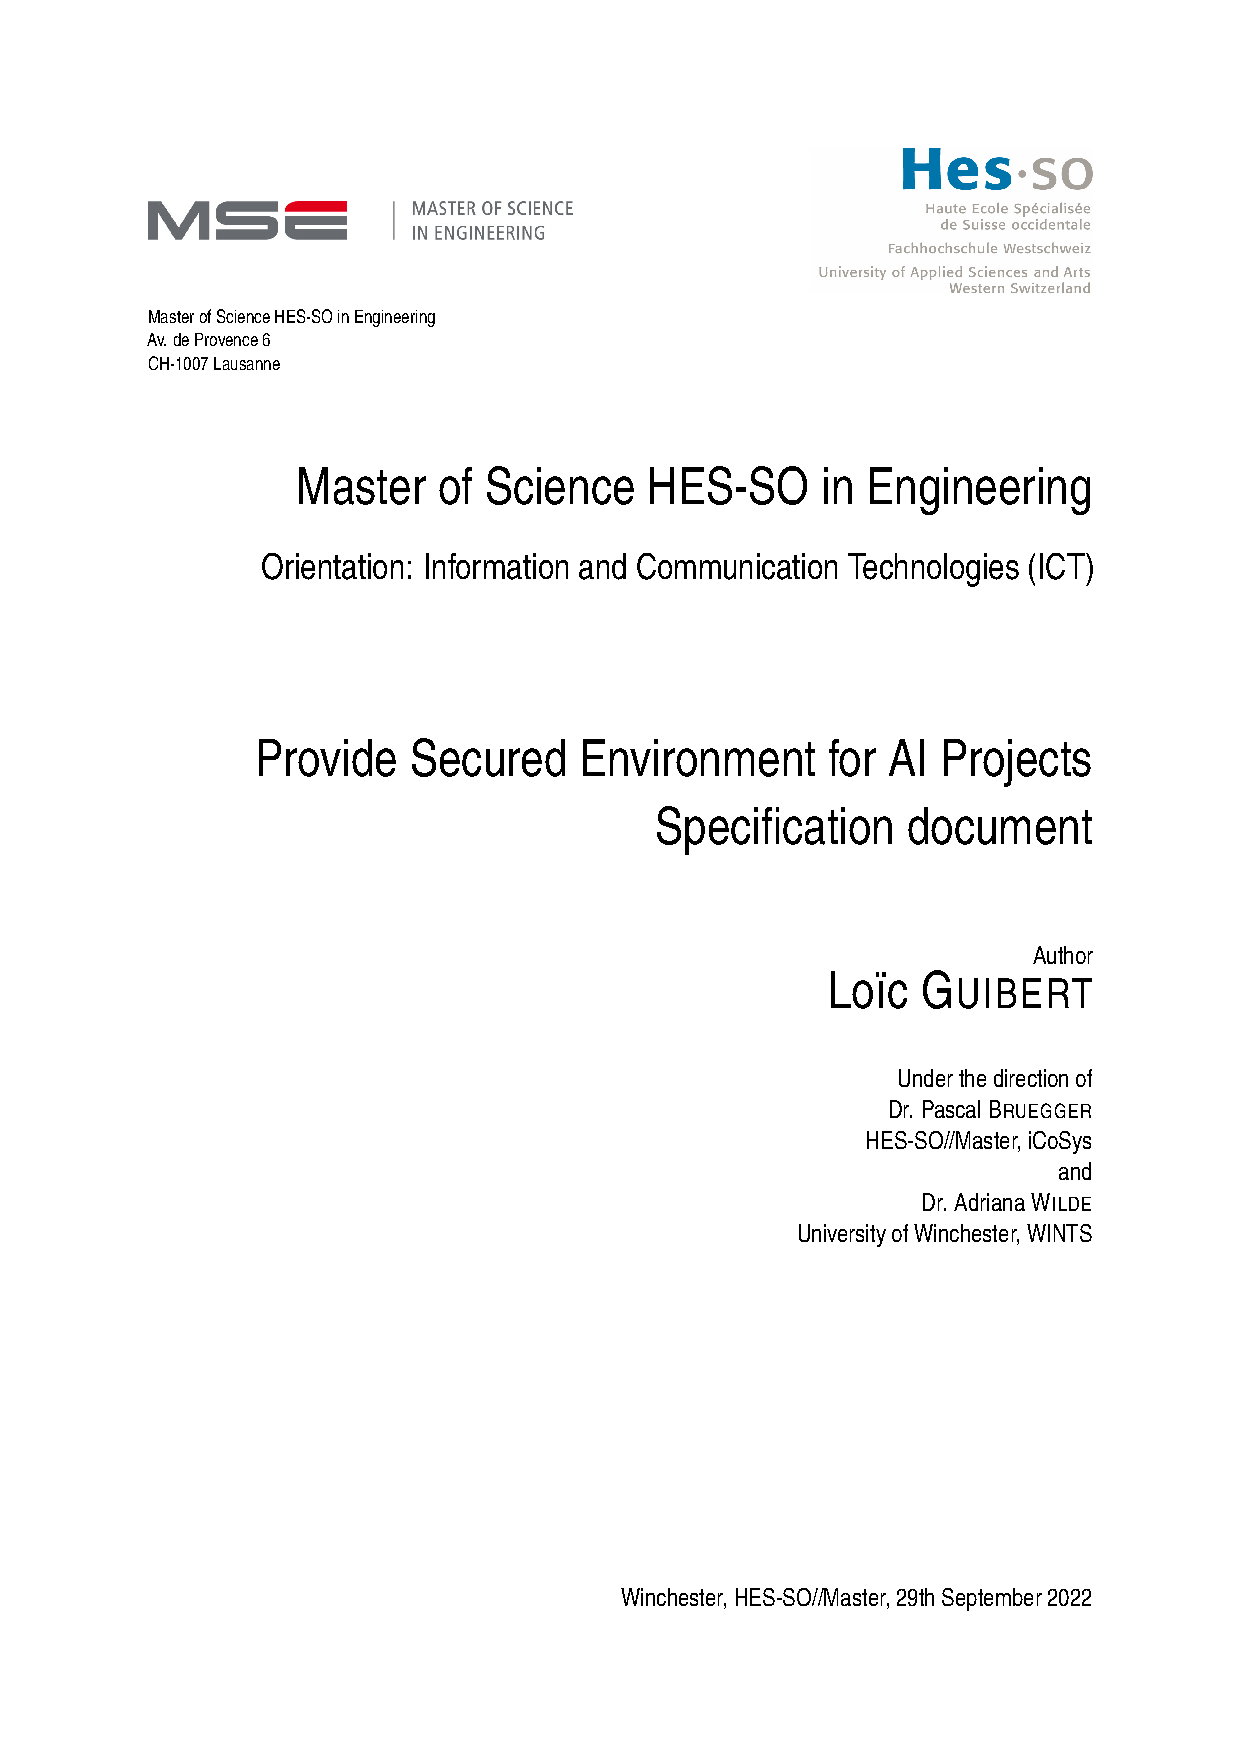
\includepdf[pages=-]{03-tail/appendices/specifications.pdf}

% -----------------------------------------------------------------------------
\newappendix{Guide Content}
\label{appendix:guide}

%TODO
The next fifty pages present the spreadsheet file acting as the dataset that has been defined during this thesis.

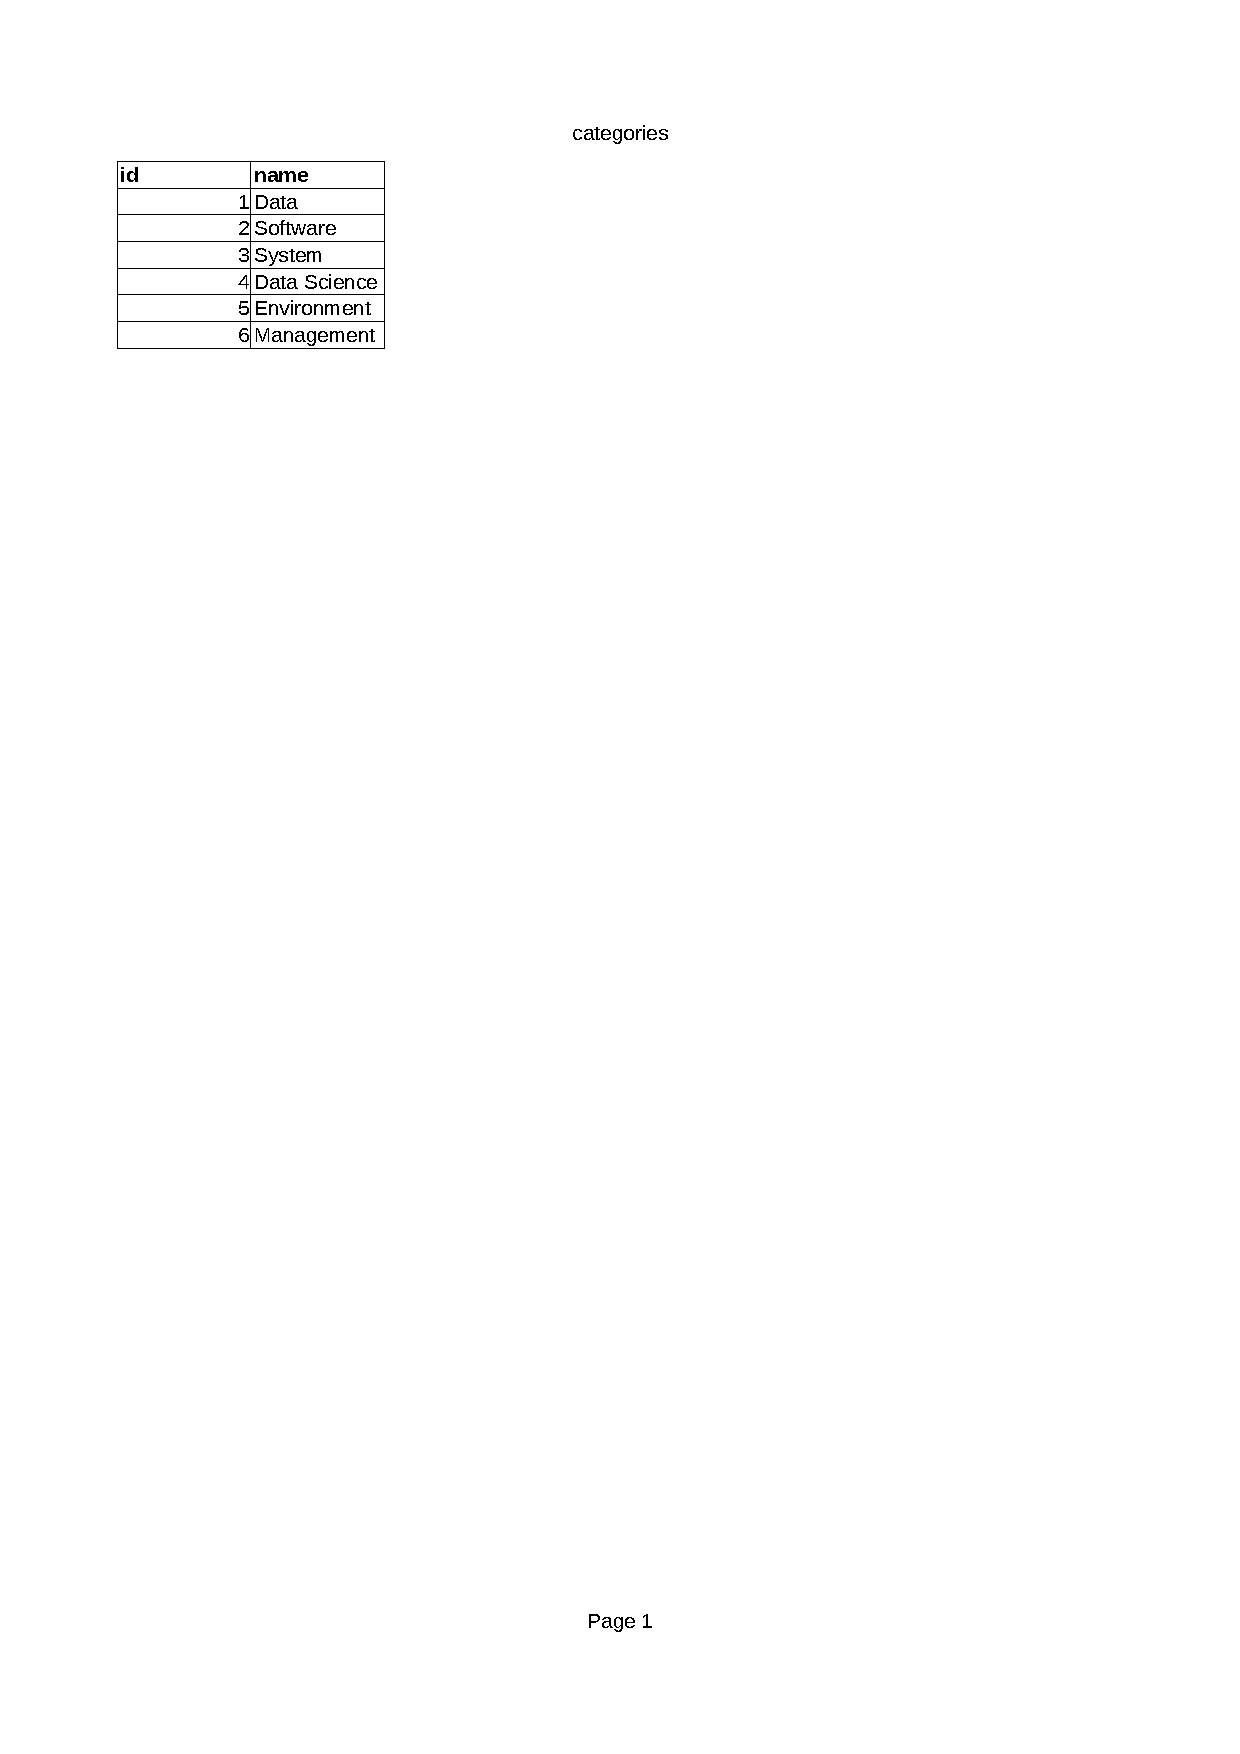
\includepdf[pages={-},fitpaper,rotateoversize]{03-tail/appendices/dataset.pdf}

% -----------------------------------------------------------------------------
\newappendix{Software Tests}
\label{appendix:tests}

\captionsetup[table]{list=no}

% Counters 
\newcounter{testsdatacounter}
\newcounter{testsappcounter}

The results of the conducted software tests are summarized in this appendix.

\begin{hyphenrules}{nohyphenation}
	\begin{table}[ht]
		\begin{center}
			\begin{tabularx}{\textwidth}{l|p{4cm}Xc}
				\toprule[0.8mm]
				\textbf{ID} & \textbf{Action} & \textbf{Expected result} & \textbf{Result} \\
				\midrule[0.8mm] 
				\stepcounter{testsdatacounter}
				1.\thetestsdatacounter & Run script with valid arguments & The arguments are passed to the script and used by it & \cellcolor{green!25}OK \\
				\midrule 
				\stepcounter{testsdatacounter}
				1.\thetestsdatacounter & Run script with invalid arguments & The script exits after showing the arguments & \cellcolor{green!25}OK \\
				\midrule 
				\stepcounter{testsdatacounter}
				1.\thetestsdatacounter & Run script without arguments & The script exits after showing the arguments & \cellcolor{green!25}OK \\
				\midrule 
				\stepcounter{testsdatacounter}
				1.\thetestsdatacounter & Run script with the \texttt{help} argument & The script exits after showing the arguments & \cellcolor{green!25}OK \\
				\midrule 
				\stepcounter{testsdatacounter}
				1.\thetestsdatacounter & Run script with as invalid \citeproper{ODS} file & The script exits after showing the reason & \cellcolor{green!25}OK \\
				\midrule 
				\stepcounter{testsdatacounter}
				1.\thetestsdatacounter & The \citeproper{ODS} file has an invalid attribute & The attribute is not processed & \cellcolor{green!25}OK \\
				\midrule 
				\stepcounter{testsdatacounter}
				1.\thetestsdatacounter & The \citeproper{ODS} file has an invalid value & The script shows the error & \cellcolor{green!25}OK \\
				\midrule 
				\stepcounter{testsdatacounter}
				1.\thetestsdatacounter & The hash is calculated based on the guide content & The hash is valid & \cellcolor{green!25}OK \\
				\bottomrule[0.8mm]
			\end{tabularx}
		\end{center}
		\caption*{Data conversion tests}
	\end{table}
\end{hyphenrules}

\begin{table}[ht]
    \begin{center}
        \begin{tabularx}{\textwidth}{l|XXc}
            \toprule[0.8mm]
            \textbf{ID} & \textbf{Action} & \textbf{Expected result} & \textbf{Result} \\
            \midrule[0.8mm] 
			\stepcounter{testsappcounter}
            2.\thetestsappcounter & Click on the evaluation button. & The \texttt{ExplanationView} page opens. & \cellcolor{green!25}OK \\
            \midrule 
			\stepcounter{testsappcounter}
            2.\thetestsappcounter & Click on the restoration button. & The \texttt{ResorationView} page opens. & \cellcolor{green!25}OK \\
            \midrule 
			\stepcounter{testsappcounter}
            2.\thetestsappcounter & Click on the report button. & The report \gls{pdf} file opens in another tab. & \cellcolor{green!25}OK \\
            \midrule 
			\stepcounter{testsappcounter}
            2.\thetestsappcounter & Click on the \gls{pwa} browser titles. & Additional installation information is shown. & \cellcolor{green!25}OK \\
            \midrule 
			\stepcounter{testsappcounter}
            2.\thetestsappcounter & Click on the \gls{pwa} links. & Links are opened in another browser tab. & \cellcolor{green!25}OK \\
            \bottomrule[0.8mm]
        \end{tabularx}
    \end{center}
    \caption*{Application tests on the \texttt{HomeView} user interface}
    \label{table:app_tests_ui_homeview}
\end{table}

\begin{hyphenrules}{nohyphenation}
\begin{table}[ht]
    \begin{center}
        \begin{tabularx}{\textwidth}{l|p{3.2cm}Xc}
            \toprule[0.8mm]
				\textbf{ID} & \textbf{Action} & \textbf{Expected result} & \textbf{Result} \\
				\midrule[0.8mm] 
				\stepcounter{testsappcounter}
				2.\thetestsappcounter & Click on the upload form. & A system modal window opens to select a \gls{json} file. & \cellcolor{green!25}OK \\
				\midrule 
				\stepcounter{testsappcounter}
				2.\thetestsappcounter & Click on the upload submit button. & The integrity of the \gls{json} file is verified, the progress or results are saved into the store and the assessor is redirected to either the \texttt{EvaluationView} page or the \texttt{ResultsView} page. & \cellcolor{green!25}OK \\
				\bottomrule[0.8mm]
        \end{tabularx}
    \end{center}
    \caption*{Application tests on the \texttt{RestoreView} user interface}
    \label{table:app_tests_ui_restoreview}
\end{table}
\end{hyphenrules}

\begin{hyphenrules}{nohyphenation}
	\begin{table}[ht]
		\begin{center}
			\begin{tabularx}{\textwidth}{l|p{4cm}Xc}
				\toprule[0.8mm]
				\textbf{ID} & \textbf{Action} & \textbf{Expected result} & \textbf{Result} \\
				\midrule[0.8mm] 
				\stepcounter{testsappcounter}
				2.\thetestsappcounter & Click on the text to change guide content. & Additional information and an upload form are shown. & \cellcolor{green!25}OK \\
				\midrule 
				\stepcounter{testsappcounter}
				2.\thetestsappcounter & Click on the upload form. & A system modal window opens to select a \gls{json} file. & \cellcolor{green!25}OK \\
				\midrule 
				\stepcounter{testsappcounter}
				2.\thetestsappcounter & Click on the upload submit button. & The integrity of the \gls{json} file is verified, the guide content is saved into the store, and the assessor is redirected to the \texttt{EvaluationView} page. & \cellcolor{green!25}OK \\
				\midrule 
				\stepcounter{testsappcounter}
				2.\thetestsappcounter & Click on an item of the guide example. & If at least one description exists for the item, the item expends to give additional information, and collapses back on second click. & \cellcolor{green!25}OK \\
				\midrule 
				\stepcounter{testsappcounter}
				2.\thetestsappcounter & Click on an item checkbox of the guide example. & The store state is not updated. & \cellcolor{green!25}OK \\
				\midrule 
				\stepcounter{testsappcounter}
				2.\thetestsappcounter & Click on the evaluation button. & The \texttt{EvaluationView} page opens. & \cellcolor{green!25}OK \\
				\bottomrule[0.8mm]
			\end{tabularx}
		\end{center}
		\caption*{Application tests on the \texttt{ExplanationView} user interface}
		\label{table:app_tests_ui_explanationview}
	\end{table}
\end{hyphenrules}

\begin{hyphenrules}{nohyphenation}
	\begin{table}[ht]
		\begin{center}
			\begin{tabularx}{\textwidth}{l|p{4cm}Xc}
				\toprule[0.8mm]
				\textbf{ID} & \textbf{Action} & \textbf{Expected result} & \textbf{Result} \\
				\midrule[0.8mm] 
				\stepcounter{testsappcounter}
				2.\thetestsappcounter & Click on a subcategory name in the \texttt{Sidebar}. & Objectives, items and descriptions of the subcategory are displayed. & \cellcolor{green!25}OK \\
				\midrule 
				\stepcounter{testsappcounter}
				2.\thetestsappcounter & Click on the close option in the expended \texttt{Sidebar}. & The \texttt{Sidebar} is hidden. & \cellcolor{green!25}OK \\
				\midrule 
				\stepcounter{testsappcounter}
				2.\thetestsappcounter & Click on the expend icon to collapse the \texttt{Sidebar}. & The \texttt{Sidebar} is expended. & \cellcolor{green!25}OK \\
				\midrule 
				\stepcounter{testsappcounter}
				2.\thetestsappcounter & Click on a collapsed category in the \texttt{Sidebar}. & The group containing children of the category is expended. & \cellcolor{green!25}OK \\
				\midrule 
				\stepcounter{testsappcounter}
				2.\thetestsappcounter & Click on an expended category in the \texttt{Sidebar}. & The group containing children of the category is collapsed. & \cellcolor{green!25}OK \\
				\midrule 
				\stepcounter{testsappcounter}
				2.\thetestsappcounter & Click on the results button in the \texttt{Sidebar}. & If the evaluation is complete, the \texttt{ResultsView} page opens. & \cellcolor{green!25}OK \\
				\midrule 
				\stepcounter{testsappcounter}
				2.\thetestsappcounter & Click on the saving button in the \texttt{Sidebar}. & A \gls{json} file is downloaded containing the evaluation progress and the guide content. & \cellcolor{green!25}OK \\
				\midrule 
				\stepcounter{testsappcounter}
				2.\thetestsappcounter & Click on an item. & If at least one description exists for the item, the item expends to give additional information, and collapses back on second click. & \cellcolor{green!25}OK \\
				\midrule 
				\stepcounter{testsappcounter}
				2.\thetestsappcounter & Click on an item checkbox. & The store state is updated, and the checkbox is updated with the corresponding state value. & \cellcolor{green!25}OK \\
				\midrule 
				\stepcounter{testsappcounter}
				2.\thetestsappcounter & Click on an item checkbox. & The evaluation values change accordingly (unchecked to compliant, compliant to non-compliant, non-compliant to not concerned, not concerned to compliant). & \cellcolor{green!25}OK \\
				\midrule 
				\stepcounter{testsappcounter}
				2.\thetestsappcounter & Click on a description link. & Links are opened in another browser tab. & \cellcolor{green!25}OK \\
				\midrule 
				\stepcounter{testsappcounter}
				2.\thetestsappcounter & The last item of a subcategory is evaluated. & The corresponding subcategory is shown as completed in the \texttt{Sidebar}. & \cellcolor{green!25}OK \\
				\midrule 
				\stepcounter{testsappcounter}
				2.\thetestsappcounter & The last item of a category is evaluated. & The corresponding category is shown as completed in the \texttt{Sidebar}. & \cellcolor{green!25}OK \\
				\midrule 
				\stepcounter{testsappcounter}
				2.\thetestsappcounter & The last item of the guide is evaluated. & The result button is activated. & \cellcolor{green!25}OK \\
				\bottomrule[0.8mm]
			\end{tabularx}
		\end{center}
		\caption*{Application tests on the \texttt{EvaluationView} user interface}
		\label{table:app_tests_ui_evaluationview}
	\end{table}
\end{hyphenrules}

\begin{table}[ht]
    \begin{center}
        \begin{tabularx}{\textwidth}{l|XXc}
            \toprule[0.8mm]
            \textbf{ID} & \textbf{Action} & \textbf{Expected result} & \textbf{Result} \\
            \midrule[0.8mm] 
			\stepcounter{testsappcounter}
            2.\thetestsappcounter & If displayed, click on the non-compliant button. & The page scrolls to the non-compliant items. & \cellcolor{green!25}OK \\
			\midrule 
			\stepcounter{testsappcounter}
            2.\thetestsappcounter & Click on the download button. & A \gls{json} file is downloaded containing the evaluation progress and the guide content. & \cellcolor{green!25}OK \\
			\midrule 
			\stepcounter{testsappcounter}
			2.\thetestsappcounter & Click on the evaluation button. & The \texttt{EvaluationView} page opens. & \cellcolor{green!25}OK \\
            \bottomrule[0.8mm]
        \end{tabularx}
    \end{center}
    \caption*{Application tests on the \texttt{ResultsView} user interface}
    \label{table:app_tests_ui_resultview}
\end{table}

\begin{table}[ht]
    \begin{center}
        \begin{tabularx}{\textwidth}{l|XXc}
            \toprule[0.8mm]
            \textbf{ID} & \textbf{Action} & \textbf{Expected result} & \textbf{Result} \\
            \midrule[0.8mm]
			\stepcounter{testsappcounter}
            2.\thetestsappcounter & Click on the \gls{gasp} logo. & The \texttt{HomeView} page opens. & \cellcolor{green!25}OK \\
			\midrule 
			\stepcounter{testsappcounter}
            2.\thetestsappcounter & The assessor changes the browser size. & The user interface is responsive. & \cellcolor{green!25}OK \\
			\midrule 
			\stepcounter{testsappcounter}
            2.\thetestsappcounter & The assessor installs the \gls{pwa}. & The \gls{pwa} is installed. & \cellcolor{green!25}OK \\
            \bottomrule[0.8mm]
        \end{tabularx}
    \end{center}
    \caption*{Application tests on the general user interface}
    \label{table:app_tests_ui_general}
\end{table}

\begin{hyphenrules}{nohyphenation}
	\begin{table}[ht]
		\begin{center}
			\begin{tabularx}{\textwidth}{l|p{4cm}Xc}
				\toprule[0.8mm]
				\textbf{ID} & \textbf{State} & \textbf{Expected result} & \textbf{Result} \\
				\midrule[0.8mm]
				\stepcounter{testsappcounter}
				2.\thetestsappcounter & The application is accessed. & The store is initialized and filled with data. & \cellcolor{green!25}OK \\
				\midrule 
				\stepcounter{testsappcounter}
				2.\thetestsappcounter & The application is accessed. & The values of the items are undefined. & \cellcolor{green!25}OK \\
				\midrule 
				\stepcounter{testsappcounter}
				2.\thetestsappcounter & A \gls{json} file is processed. & The data are verified on its integrity. & \cellcolor{green!25}OK \\
				\midrule 
				\stepcounter{testsappcounter}
				2.\thetestsappcounter & A \gls{json} file contains an error. & A comprehensive and detailed error dialogue is shown. & \cellcolor{green!25}OK \\
				\midrule 
				\stepcounter{testsappcounter}
				2.\thetestsappcounter & A restoration is done for a custom or an older version of the guide content. & The custom or older version of the guide content is loaded into the store and an information message is shown. & \cellcolor{green!25}OK \\
				\midrule 
				\stepcounter{testsappcounter}
				2.\thetestsappcounter & The \texttt{EvaluationView} is opened. & A default subcategory is displayed. & \cellcolor{green!25}OK \\
				\midrule 
				\stepcounter{testsappcounter}
				2.\thetestsappcounter & The \texttt{EvaluationView} is opened. & The \texttt{Sidebar} is displayed. & \cellcolor{green!25}OK \\
				\midrule 
				\stepcounter{testsappcounter}
				2.\thetestsappcounter & The evaluation is not complete. & The \texttt{ResultsView} is not accessible and a redirection to \texttt{EvaluationView} is made. & \cellcolor{green!25}OK \\
				\midrule 
				\stepcounter{testsappcounter}
				2.\thetestsappcounter & The results are shown. & The colour of the progress change based on their value (less than 50\% in red, less than 85\% in orange, less than 100\% in green, 100\% in dark green). & \cellcolor{green!25}OK \\
				\midrule 
				\stepcounter{testsappcounter}
				2.\thetestsappcounter & The overall score is not of 100\%. & The non-compliant items are shown. & \cellcolor{green!25}OK \\
				\midrule 
				\stepcounter{testsappcounter}
				2.\thetestsappcounter & A mobile phone is used. & The user interface is responsive. & \cellcolor{green!25}OK \\
				\bottomrule[0.8mm]
			\end{tabularx}
		\end{center}
		\caption*{Application tests on its behaviour}
		\label{table:app_tests_behaviour}
	\end{table}
\end{hyphenrules}

\begin{table}[ht]
    \begin{center}
        \begin{tabularx}{\textwidth}{l|lXc}
            \toprule[0.8mm]
            \textbf{ID} & \textbf{Object} & \textbf{Expected result} & \textbf{Result} \\
            \midrule[0.8mm]
			\stepcounter{testsappcounter}
            2.\thetestsappcounter & Guide content & Integrity checks are realized before storing the guide content. & \cellcolor{green!25}OK \\
			\midrule
			\stepcounter{testsappcounter}
            2.\thetestsappcounter & Evaluation status & When complete, the store changes the status of the evaluation. & \cellcolor{green!25}OK \\
			\midrule
			\stepcounter{testsappcounter}
            2.\thetestsappcounter & Category status & When complete, the store changes the status of the corresponding category. & \cellcolor{green!25}OK \\
			\midrule
			\stepcounter{testsappcounter}
            2.\thetestsappcounter & Subcategory status & When complete, the store changes the status of the corresponding subcategory. & \cellcolor{green!25}OK \\
			\midrule
			\stepcounter{testsappcounter}
            2.\thetestsappcounter & Score computation & The score computation is done accordingly to the defined formula from the proposal. & \cellcolor{green!25}OK \\
			\midrule
			\stepcounter{testsappcounter}
            2.\thetestsappcounter & Object getters & The store getters can return lists of all objects or of filtered objects giving unique identifiers. & \cellcolor{green!25}OK \\
			\midrule
			\stepcounter{testsappcounter}
            2.\thetestsappcounter & Object types and classes. & The store getters and its related data are using the appropriate \gls{typescript} types and classes. & \cellcolor{green!25}OK \\
            \bottomrule[0.8mm]
        \end{tabularx}
    \end{center}
    \caption*{Application tests on the store}
    \label{table:app_tests_store}
\end{table}

% -----------------------------------------------------------------------------
\newappendix{Project Management}
\label{appendix:project}

\begin{itemize}
	\item The next image shows some statistics of the activities done on the thesis repository~\cite{mt-forge}.
	\item The next page is the Gantt planning representing our thesis progress. Its originally planned version can be consulted at \appendixref{appendix:specifications}.
	\item The minutes of the meetings done during the thesis can be consulted on the thesis repository~\cite{mt-forge}.
\end{itemize}

\vspace{5cm}

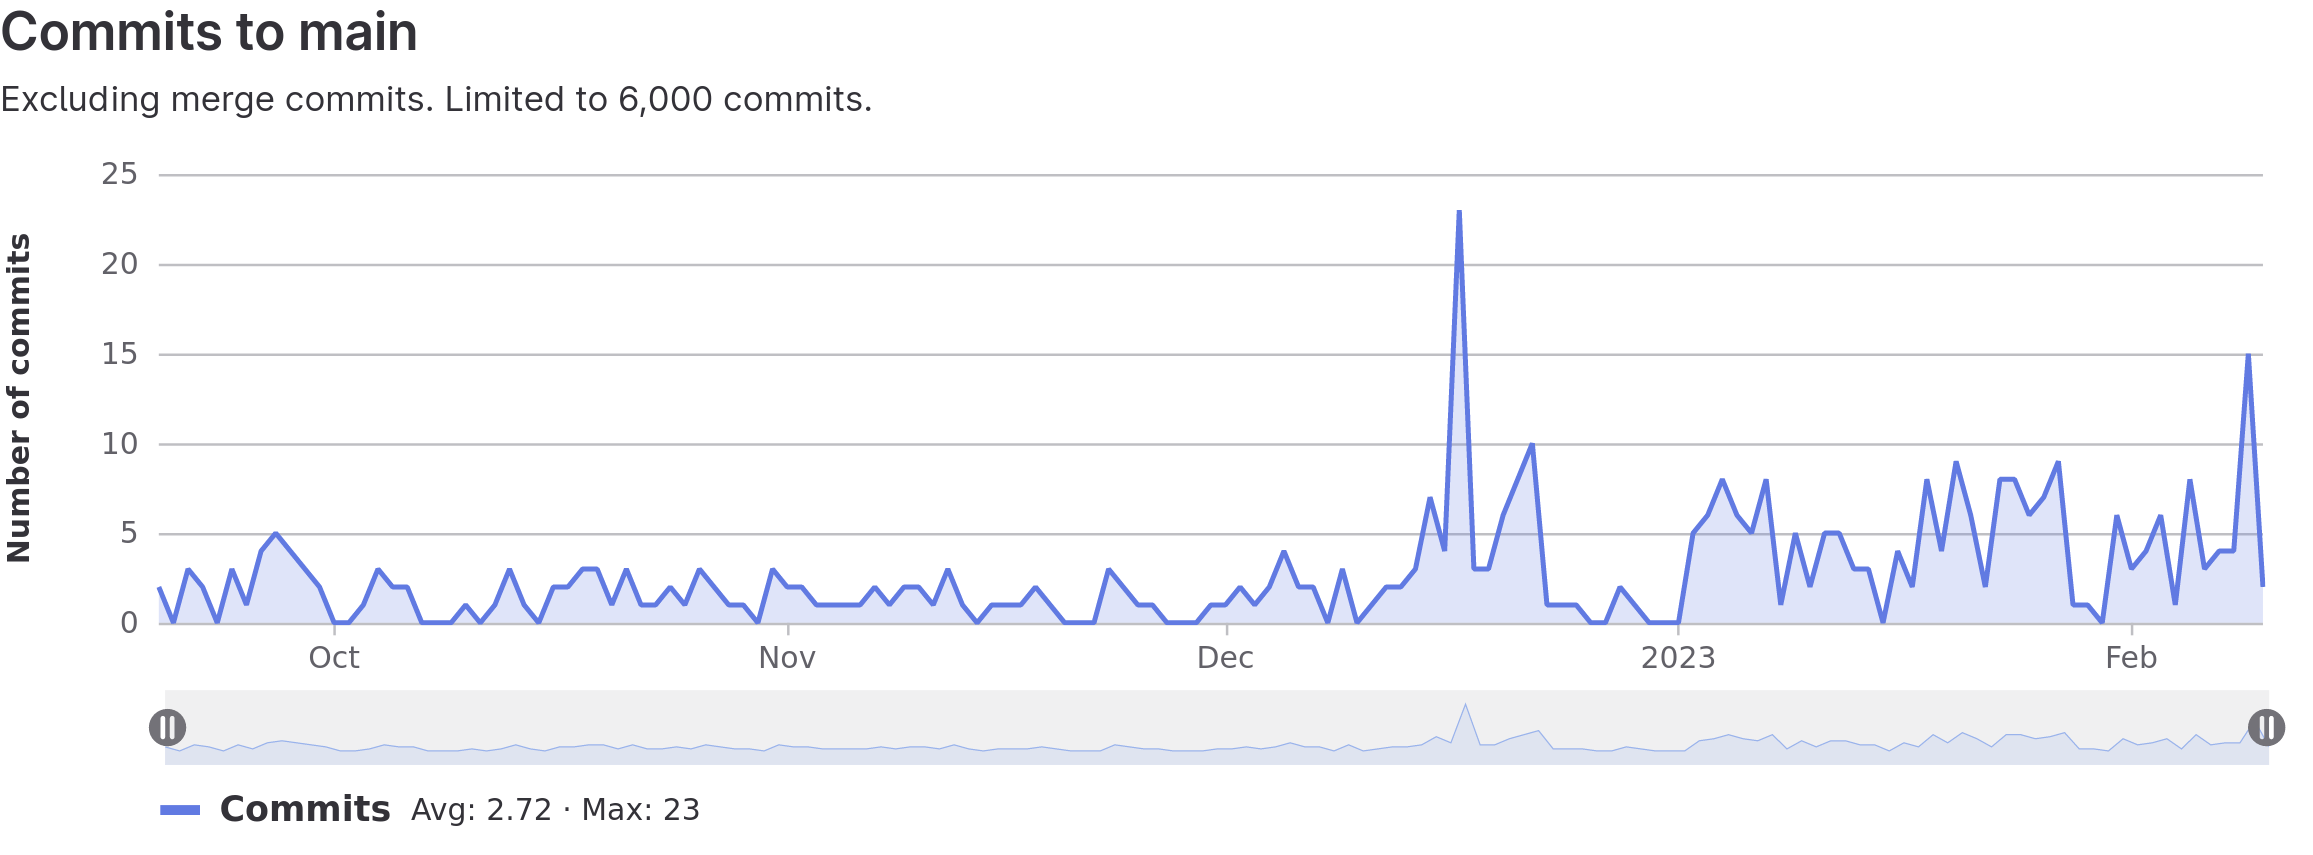
\includegraphics[width=1\textwidth]{03-tail/appendices/repository.png}

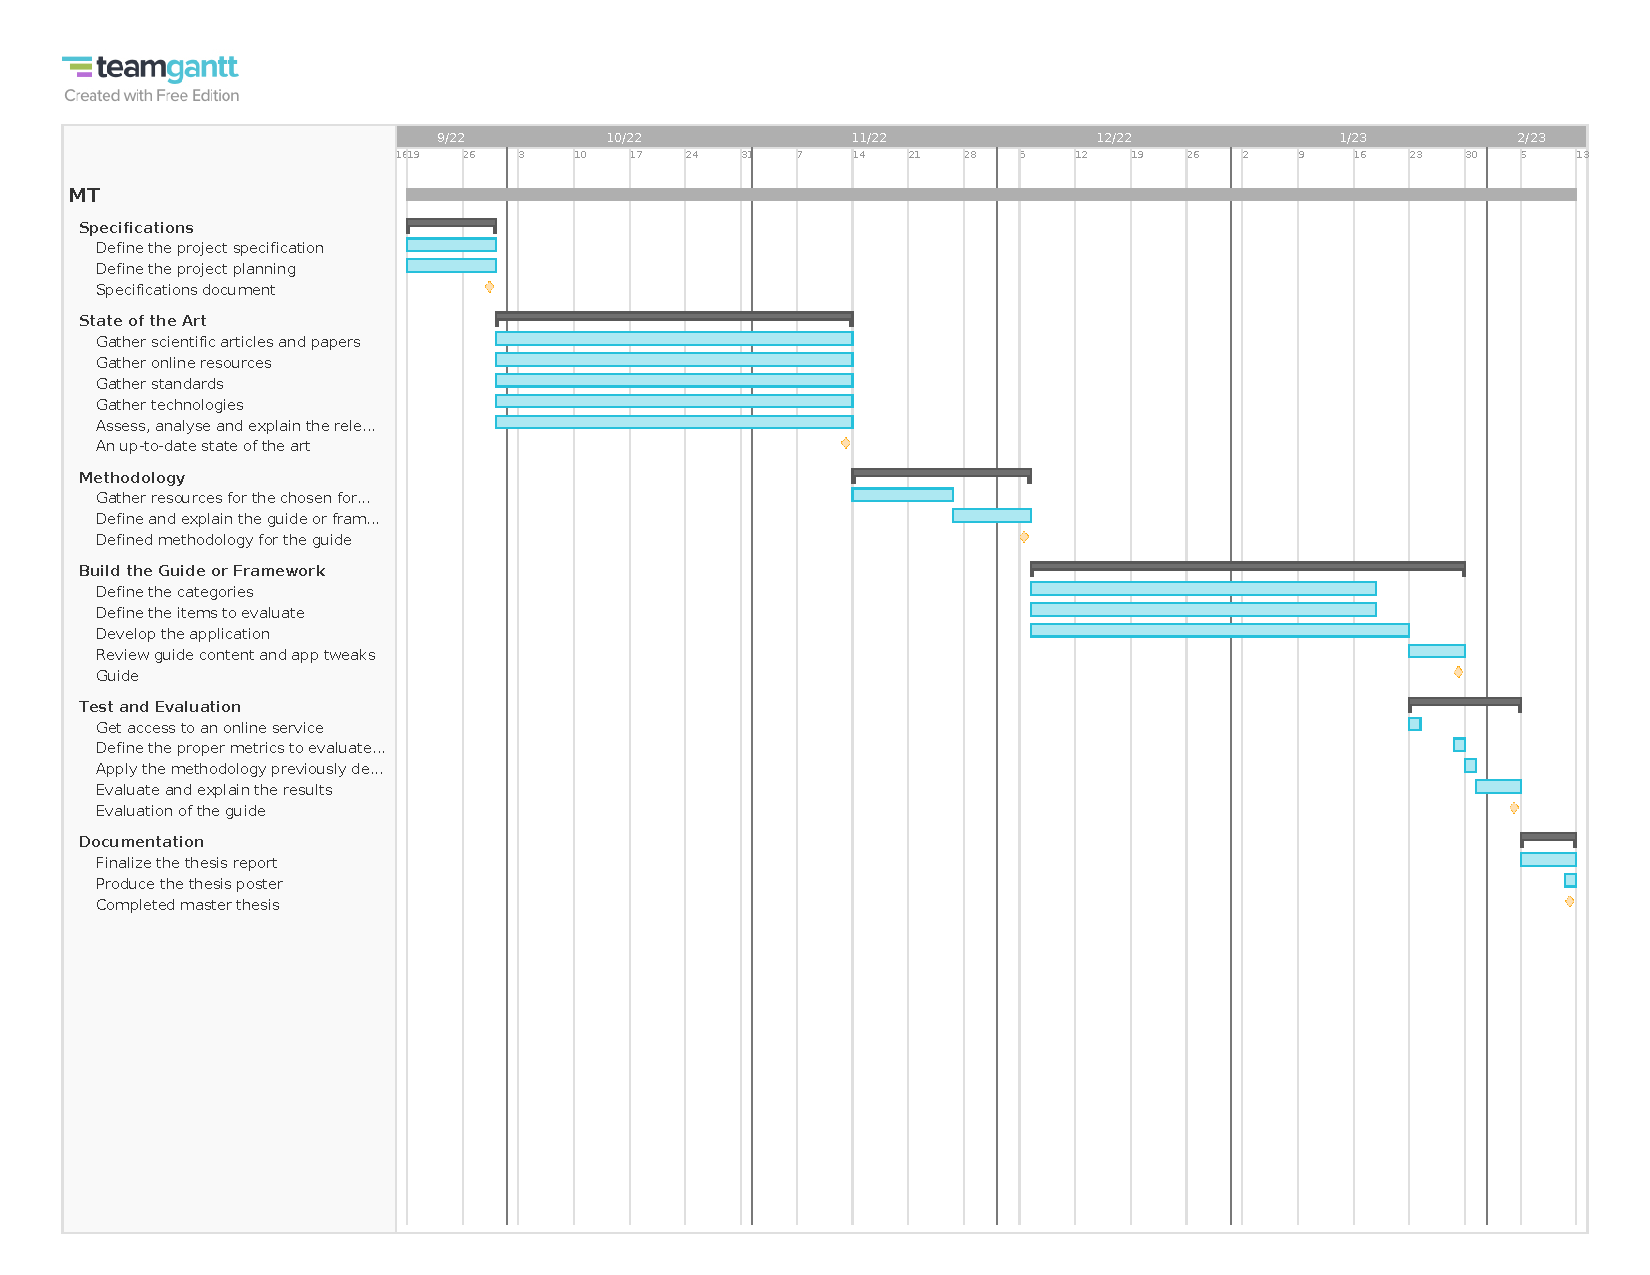
\includepdf[pages={-},angle=90]{03-tail/appendices/gantt_final.pdf}

% -----------------------------------------------------------------------------
\newappendix{Software and Tools}
\label{appendix:software}

This appendix does not list the software dependencies or tools if they have already been presented before in this report.

\subsection*{Office Tools}

All the software and tools used for the administrative or documentation tasks are listed here.

\citeproper{\LaTeX \ Suite - pdfTeX}, used to generate the documents for this project.

\begin{itemize}
	\item Version 3.141592653-2.6-1.40.22 (TeX Live 2021)
	\item Licence pdfTeX copyright, Lesser GNU General Public
\end{itemize}


\citeproper{Zotero}, used to manage the dissertation references.

\begin{itemize}
	\item Version 6.0.13
	\item Licence AGPL-3.0
\end{itemize}


\citeproper{Draw.io}, used to draw the different graphs.

\begin{itemize}
	\item Version 19.0.0
	\item Licence APACHE Licence, version 2.0
\end{itemize}


\citeproper{Microsoft Teams}, used to conduct organizational and follow-up sessions.

\begin{itemize}
	\item Version 1.5.00.10453 (64-bit) (64 bits)
	\item Licence Proprietary
\end{itemize}

\newpage

\subsection*{Development Tools}

All the software and tools used for the development tasks are listed here.

\citeproper{LibreWolf}, used for research, implementation and testing.

\begin{itemize}
	\item Version from 104.0.2-1
	\item Licence MPL-2.0 (d), GNU General Public Licence (GPL) et GNU Lesser General Public Licence (LGPL)
\end{itemize}


\citeproper{ungoogled-chromium}, used for research, implementation and testing.

\begin{itemize}
	\item Version 105.0.5195.125
	\item Licence BSD-3-Clause
\end{itemize}


\citeproper{GitLab}, used to manage the versioning of project resources.

\begin{itemize}
	\item Version GitLab Enterprise Edition 15.3.2-ee
	\item Licence MIT Licence
\end{itemize}


\citeproper{VSCodium}, used to implement \citeproper{JavaScript} software and to redact the \LaTeX documents.

\begin{itemize}
	\item Version 1.71.2
	\item Licence MIT Licence
\end{itemize}


\citeproper{PyCharm Professional}, used to implement the \citeproper{Python} script.

\begin{itemize}
	\item Version 2022.2.4
	\item Licence Copyright © 2010-2022 JetBrains s.r.o.
\end{itemize}


\citeproper{LibreOffice Calc}, used to create the spreadsheet file.

\begin{itemize}
	\item Version 7.4.3.2
	\item Licence MPL-2.0
\end{itemize}

\end{document}